%%%%%%%%%%%%%%%%%%%%%%%%%%%%%%%%%%%%%%%%%%%%%%%%%%%%%%%%%%%%%%%%%%%%%%%%%%%%%%%%%%%%%%%%%%%%%%%%%%%%%%%
%%                                                                                                   %%
%%                                          DIPLOMOVÁ PRÁCE                                          %%
%%                                           Michal Kovář                                            %%
%%                                                                                                   %%
%% pro formátování využita šablona: http://geo3.fsv.cvut.cz/kurzy/mod/resource/view.php?id=775       %%
%%                                  https://people.fsv.cvut.cz/~soukup/dip/horcickova/horcickova.pdf %%
%%                                                                                                   %%
%%%%%%%%%%%%%%%%%%%%%%%%%%%%%%%%%%%%%%%%%%%%%%%%%%%%%%%%%%%%%%%%%%%%%%%%%%%%%%%%%%%%%%%%%%%%%%%%%%%%%%%
\documentclass[
  12pt,         			% Velikost základního písma je 12 bodů
  a4paper,      			% Formát papíru je A4
  oneside,       			% Oboustranný tisk
  pdftex,				    % Překlad bude proveden programem 'pdftex' do PDF
% twoside                   % Zarovnaní stran pro oboustranný tisk
]{report}       		    % Dokument třídy 'zpráva'

\newcommand{\Fbox}[1]{\fbox{\strut#1}}

\usepackage[czech, english]{babel}	% použití češtiny, angličtiny
\usepackage[utf8]{inputenc}		% Kódování zdrojových souborů je UTF8

\usepackage[square,sort,comma,numbers]{natbib}

\usepackage{caption}
\usepackage{subcaption}
\captionsetup{font=small}
\usepackage{enumitem} 
\setlist{leftmargin=*} % bez odsazení

\makeatletter
\setlength{\@fptop}{0pt}
\setlength{\@fpbot}{0pt plus 1fil}
\makeatletter

\usepackage{graphicx}   
\usepackage{color}
\usepackage{transparent}
\usepackage{wrapfig}
\usepackage{float} 

\usepackage{cmap}           
\usepackage[T1]{fontenc}    

\usepackage{textcomp}
\usepackage[compact]{titlesec}
\usepackage{amsmath}
\addtolength{\jot}{1em} 

\usepackage{chngcntr}
\counterwithout{footnote}{chapter}

\usepackage{acronym}

\usepackage[nopatch]{microtype}

\usepackage[
    unicode,                
    breaklinks=true,        
    hypertexnames=false,
    colorlinks=true, % true for print version
    citecolor=black,
    filecolor=black,
    linkcolor=black,
    urlcolor=black
]{hyperref}         

\usepackage{url}
\usepackage{fancyhdr}
%\usepackage{algorithmic}
\usepackage{algorithm}
\usepackage{algcompatible}
\renewcommand{\ALG@name}{Pseudokód}% Update algorithm name
\def\ALG@name{Pseudokód}

%%%%%%%%%%%%%%%%%%%%%%%%%%%%%%%%%%%%%%%%%%%%%%%%%%%%%%%%%%%%%%%%%%%%%%%%%%%%%%%%%%%%%%%%%%%%%%%%%%%%%%%
%%                                                                                                   %%
%%                                   úpravy šablony - Michal Kovář                                   %%
%%                                                                                                   %%
%%                     Tip: pro zalomování text v *.tex ve vscode zkratka ALT + Z                    %%

\overfullrule=5pt
\hfuzz=0pt
\hbadness=1000

\usepackage{pdfpages}% pro přidání celé stránky pdf na radu Filipa
\usepackage{dirtree}% pro tvorubu struktury adresáře
\newcommand\dottedline{\leavevmode\cleaders\hbox to 2.9mm{\hfil.\hfil}\hfill\kern0pt}
\usepackage{marvosym}% znak eura a jarního bodu
\usepackage{qrcode} %tvorba QR kodu na který lze i kliknout
\usepackage{tikz}
\usetikzlibrary{shapes.geometric, arrows}
\usepackage{tikz-3dplot}
\usepackage{eurosym}% pro symbol eura
\usepackage{ragged2e}% pro vyrovnání do bloku příkazem \justifying
\usepackage{listings}%pro psaní kodu
\usepackage{hyphenat}% na radu od Filipa pro nazalomování slov

\usepackage{multirow}
\usepackage{tabularx}

\usetikzlibrary{positioning}

\usepackage{lmodern} %pro hezčí font na mikTeXu

\usepackage{xparse}% pro volitelné argumenty

\usepackage{minted}%barevná syntaxe kodu
\usepackage{listings}
\usepackage{xcolor}
\lstdefinestyle{python}{
    language=Python,
    basicstyle=\small\ttfamily,
    keywordstyle=\color{blue}\bfseries,
    stringstyle=\color{orange},
    commentstyle=\color{gray}\itshape,
    frame=lines,
    numbers=left,
    numberstyle=\tiny\color{gray},
    showstringspaces=false,
}

%zalamování url v bib
\usepackage{hyperref}
\usepackage{xurl}   % nejlepší zalamování URL

\usepackage{booktabs}

% Definice vlastního příkazu \tg a \cotg
\newcommand{\tg}{\mathrm{tg}}                                                                        %%
\newcommand{\cotg}{\mathrm{cotg}}                                                                    %%
%%%%%%%%%%%%%%%%%%%%%%%%%%%%%%%%%%%%%%%%%%%%%%%%%%%%%%%%%%%%%%%%%%%%%%%%%%%%%%%%%%%%%%%%%%%%%%%%%%%%%%%

\usepackage[
  cvutstyle,          
  diploma           
]{thesiscvut}


\newif\ifweb
\ifx\ifHtml\undefined % Mimo HTML.
    \webfalse
\else % V HTML.
    \webtrue
\fi 

\renewcommand{\figurename}{Obrázek}
\def\figurename{Obrázek}

%%%%%%%%%%%%%%%%%%%%%%%%%%%%%%%%%%%%%%%%%%%%%%%%%%%%%%%%%%%%%%%%%
%%%%%%%%%%% Definice informací o dokumentu  %%%%%%%%%%%%%%%%%%%%%
%%%%%%%%%%%%%%%%%%%%%%%%%%%%%%%%%%%%%%%%%%%%%%%%%%%%%%%%%%%%%%%%%

%% Název práce
\nazev{Analýza výsledků zpracování metody DORIS (Doppler Orbitography and Radiopositioning Integrated by Satellite)}
{sdgfdg}%Analýza výsledků zpracování metody DORIS (Doppler Orbitography and Radiopositioning Integrated by Satellite)

% Jméno a příjmení autora
\autor{Bc.~Michal}{Kovář}

% %% Jméno a příjmení vedoucího práce včetně titulů
\garant{doc.~Ing.~Jakub~Kostelecký,~Ph.D. a Ing.~Petr~Štěpánek,~Ph.D.}

%% Označení programu studia
\programstudia{Geodézie a~kartografie}{}

%% Označení oboru studia
\oborstudia{GEODÉZIE, KARTOGRAFIE A~GEOINFORMATIKA}{}

%% Označení ústavu
\ustav{Katedra geomatiky}{}

%% Rok obhajoby
\rok{\the\year}

%Mesic obhajoby
\mesic{červen}

%% Místo obhajoby
\misto{Praha}
%% Abstrakt
\abstrakt
{Tato diplomová práce se zabývá analýzou výsledků zpracování metody DORIS (Doppler Orbitography and Radiopositioning Integrated by Satellite), s~důrazem na výstupy analytického centra systému DORIS na Geodetické observatoři Pecný. První část práce se zaměřuje na analýzu časových řad souřadnic stanic systému DORIS a na určení dlouhodobých trendů, diskontinuit a periodických složek. Druhá část práce se zaměřuje na analýzu přesných drah družic vybavených přijímačem systému DORIS. Pro porovnání drah jsou využity dva přístupy – dynamická parametrizace dráhy v~Bernese GNSS Software a Hermitova interpolace souřadnic v~daných epochách.}
{This master’s thesis deals with the analysis of the results of DORIS (Doppler Orbitography and Radiopositioning Integrated by Satellite) processing, with emphasis on the outputs of the DORIS Analysis Center at the Geodetic Observatory Pecný. The first part of the thesis focuses on the analysis of time series of DORIS station coordinates and on the identification of long-term trends, discontinuities, and periodic components. The second part of the thesis focuses on the analysis of precise orbits of satellites equipped with DORIS receivers. For orbit comparison, two approaches are used – dynamic orbit parameterization in the Bernese GNSS Software and Hermite interpolation of coordinates at given epochs.}

%% Klíčová slova
\klicovaslova
{DORIS, IDS, časové řady, souřadnice stanic, přesné dráhy družic, detekce diskontinuit, trendová analýza, spektrální analýza, Bernese GNSS Software, interpolace drah}
{DORIS, IDS, time series, station coordinates, precise satellite orbits, discontinuity detection, trend analysis, spectral analysis, Bernese GNSS Software, orbit interpolation}

%%%%%%%%%%%%%%%%%%%%%%%%%%%%%%%%%%%%%%%%%%%%%%%%%%%%%%%%%%%%%%%%%%%%%%%%

%%%%%%%%%%%%%%%%%%%%%%%%%%%%%%%%%%%%%%%%%%%%%%%%%%%%%%%%%%%%%%%%%%%%%%%%
%% Nastavení polí ve Vlastnostech dokumentu PDF
%%%%%%%%%%%%%%%%%%%%%%%%%%%%%%%%%%%%%%%%%%%%%%%%%%%%%%%%%%%%%%%%%%%%%%%%
\nastavenipdf
%%%%%%%%%%%%%%%%%%%%%%%%%%%%%%%%%%%%%%%%%%%%%%%%%%%%%%%%%%%%%%%%%%%%%%%

%% Začátek dokumentu
\begin{document}
\selectlanguage{czech}

\catcode`\-=12  % pro vypnuti aktivniho znaku '-' pouzivaneho napr. v \cline 

% aktivace záhlaví
\zahlavi

% předefinování vzhledu záhlaví
\renewcommand{\chaptermark}[1]{%
	\markboth{\MakeUppercase
	{%
	\thechapter.%
	\ #1}}{}}

% Vysázení přebalu práce
% \vytvorobalku

% Vysázení titulní stránky práce
\vytvortitulku {}

\stranka{}%
	{\includepdf[pages=1, offset=15mm -10mm]{./images/zadani/zadani.pdf}
	}

\stranka{}%
	{\includepdf[pages=2, offset=15mm -10mm]{./images/zadani/zadani.pdf}
	}

% Vysázení stránky s abstraktem
\vytvorabstrakt

% Vysázení prohlaseni o samostatnosti
% \vytvorprohlaseni
\stranka{}%
    {
\includepdf[pages=1, offset=15mm -10mm]{./images/zadani/prohlaseni.pdf}
    }

% Vysázení poděkování
\stranka{%nahore
       }{%uprostred
       }{%dole
       \sffamily
	\begin{flushleft}
		\large
		\MakeUppercase{Poděkování}
	\end{flushleft}
	\vspace{1em}
		%\noindent
	\par\hspace{2ex}
  {Chtěl bych poděkovat svým vedoucím doc.~Ing.~Jakubu~Kosteleckému,~Ph.D., a Ing.~Petru~Štěpánkovi,~Ph.D., za jejich ochotu a množství cenných rad při vedení této diplomové práce. Velké poděkování patří také mé rodině za podporu během celého studia.}
}

% Vysázení obsahu
\obsah

% Vysázení seznamu obrázků
\seznamobrazku

% Vysázení seznamu tabulek
\seznamtabulek

% jednotlivé kapitoly
\chapter{Úvod}
\label{1-uvod}

V~posledních desetiletích došlo k~výraznému rozvoji metod kosmické geodézie. Jednou z~těchto metod je metoda \zkratka{DORIS}, která je založena na měření Dopplerova posunu signálu mezi pozemními stanicemi, na nichž jsou umístěny vysílače, a družicemi, na nichž jsou umístěny přijímače. Výsledky této metody jsou využívány například pro určování přesných drah družic, určování polohy pozemních stanic, stanovení parametrů orientace Země nebo pro realizaci a zpřesňování mezinárodního terestrického referenčního rámce (\zk{ITRF})~\cite{ids_what_is_doris}. Koordinaci zpracování a distribuci produktů systému DORIS zajišťuje služba \zkratka{IDS}, která poskytuje jednotlivé produkty, tedy výsledky zpracování analytických center. Analytická centra \zkratka{IDS} zpracovávají data nezávisle různými metodickými postupy, a proto je nutné jejich výsledky pravidelně analyzovat a vzájemně porovnávat. Kvalita těchto výstupů má přímý vliv na přesnost určení souřadnic stanic i drah družic, a tím i na kvalitu globálních geodetických produktů.

Cílem této diplomové práce je analyzovat výsledky zpracování metody \zkratka{DORIS} s~důrazem na výstupy analytického centra na Geodetické observatoři Pecný (\zk{GOP}), která je součástí Výzkumného ústavu geodetického, topografického a kartogra\-fického, v.~v.~i. První část práce je věnována analýze časových řad souřadnic stanic vysílačů systému \zkratka{DORIS} za období 2015--2025. Analyzovány jsou stanice, u~nichž bylo v~interním přehledu \zkratka{IDS} indikováno podezřelé chování. Cílem je toto chování potvrdit nebo vyvrátit a případně se pokusit nalézt jeho příčinu. V~rámci analýzy jsou identifikovány dlouhodobé trendy, diskontinuity a periodické složky časových řad. Druhá část práce se zabývá analýzou přesných drah družic vybavených přijímačem systému \zkratka{DORIS}. Porovnávány jsou dráhy z~řešení analytického centra na Geodetické observatoři Pecný (\zk{GOP}) s~řešením francouzského analytického centra (\zk{SSA}) za prvních 30 dní roku 2024. Pro porovnání je využita Hermitova interpolace. Výsledky jsou ověřeny nezávislým porovnáním pomocí dynamické parametrizace dráhy v~\zkratka{BSW}. Cílem je posoudit shodu výsledků obou analytických center.

Výsledkem práce je zhodnocení výstupů metody \zkratka{DORIS} se zaměřením na řešení analytického centra na Geodetické observatoři Pecný. Pro účely obou analýz byla vytvořena knihovna v~jazyce Python, která umožňuje jednotné zpracování dat systému \zkratka{DORIS}, jejich analýzu a~generování výstupů. Kompletní výsledky analýz jednotlivých stanic a~družic jsou obsaženy v~reportech v~přílohách práce.
\chapter{Rešerše}
\label{2-reserse}

Tato kapitola shrnuje základní informace o~systému \zkratka{DORIS} a službě \zkratka{IDS}. Dále jsou představeny existující práce zabývající se analýzou časových řad souřadnic stanic a porovnáváním přesných drah družic. V~dostupné literatuře nebyla nalezena komplexní práce, která by se zabývala současně analýzou časových řad souřadnic stanic systému \zkratka{DORIS} a porovnáním přesných drah družic z~různých analytických center \zkratka{IDS}. Existuje však řada prací, které se těmito oblastmi zabývají samostatně nebo v~širším kontextu.

\section{Základní informace o~systému DORIS}

Systém \zkratka{DORIS} je založen na využití Dopplerova jevu, k~němuž dochází v~důsledku relativního pohybu mezi pozemní vysílací stanicí a družicí vybavenou přijímačem. Pozemní stanice vysílají signál o~známé frekvenci, přičemž palubní přijímač na družici měří jeho frekvenční posun. Tento posun je přímo závislý na relativní rychlosti družice vůči stanici a představuje základní observaci využívanou při přesném určování drah družic. Systém \zkratka{DORIS} poskytuje dva typy observací, a to dopplerovská a synchronizační měření. Na palubě družice je měření realizováno sledováním fáze přijímaného signálu, přičemž změna fáze v~čase odpovídá změně frekvence, z~níž je následně odvozena Dopplerovská observace využívaná při zpracování dat. Synchronizační měření slouží především pro časovou vazbu mezi palubními a pozemními časovými škálami~\cite{ids_what_is_doris}.

\subsection{Princip měření}

Na rozdíl od globálních navigačních satelitních systémů \zk{GNSS}, kde jsou vysílače umístěny na družicích a přijímače na zemském povrchu, využívá systém \zkratka{DORIS} opačné uspořádání. Vysílače se nacházejí na pozemních stanicích, zatímco přijímače jsou umístěny na družicích. Díky tomu je technicky náročnější část systému umístěna na Zemi a na družicích se nachází konstrukčně jednodušší část systému~\cite{ids_what_is_doris}.

Pozemní stanice \zkratka{DORIS} vysílají nepřetržitý signál současně na~dvou frekvencích (2036,25~MHz a~401,25~MHz), jejichž kombinace umožňuje potlačení vlivu ionosféry~\cite{ids_frequency_shift}. Stabilita těchto vysílaných frekvencí je stěžejní pro~přesnost měření, jelikož jakákoliv nestabilita by se přímo promítla do~odhadu relativní rychlosti~\cite{ids_what_is_doris}. U~vybraných stanic se navíc využívá mírný posun frekvence oproti nominální hodnotě. To se aplikuje v~situacích, kdy se dvě stanice nacházejí v~blízké geografické poloze, čímž se předchází vzájemnému rušení signálů~\cite{ids_frequency_shift}.

Palubní přijímač na družici měří fázi přijímaného signálu, ze~které se odvozuje frekvenční posun způsobený relativním pohybem mezi družicí a stanicí. Pozemní stanice vysílá signál o~známé frekvenci \(f_0\), zatímco frekvence signálu přijímaného na družici je označena \(f_r\). Rozdíl mezi těmito frekvencemi odpovídá Dopplerovu posunu, který přímo souvisí s~relativní rychlostí družice vůči stanici. Při přibližování družice ke stanici platí \(f_r > f_0\), při vzdalování \(f_r < f_0\). Měřením časového průběhu této změny během průletu družice nad~stanicí se získává základní observace využitelná při~přesném určení dráhy družice. Schéma tohoto principu je znázorněno na obr.~\ref{fig:doris_system}.

\begin{figure}[H]
    \centering
    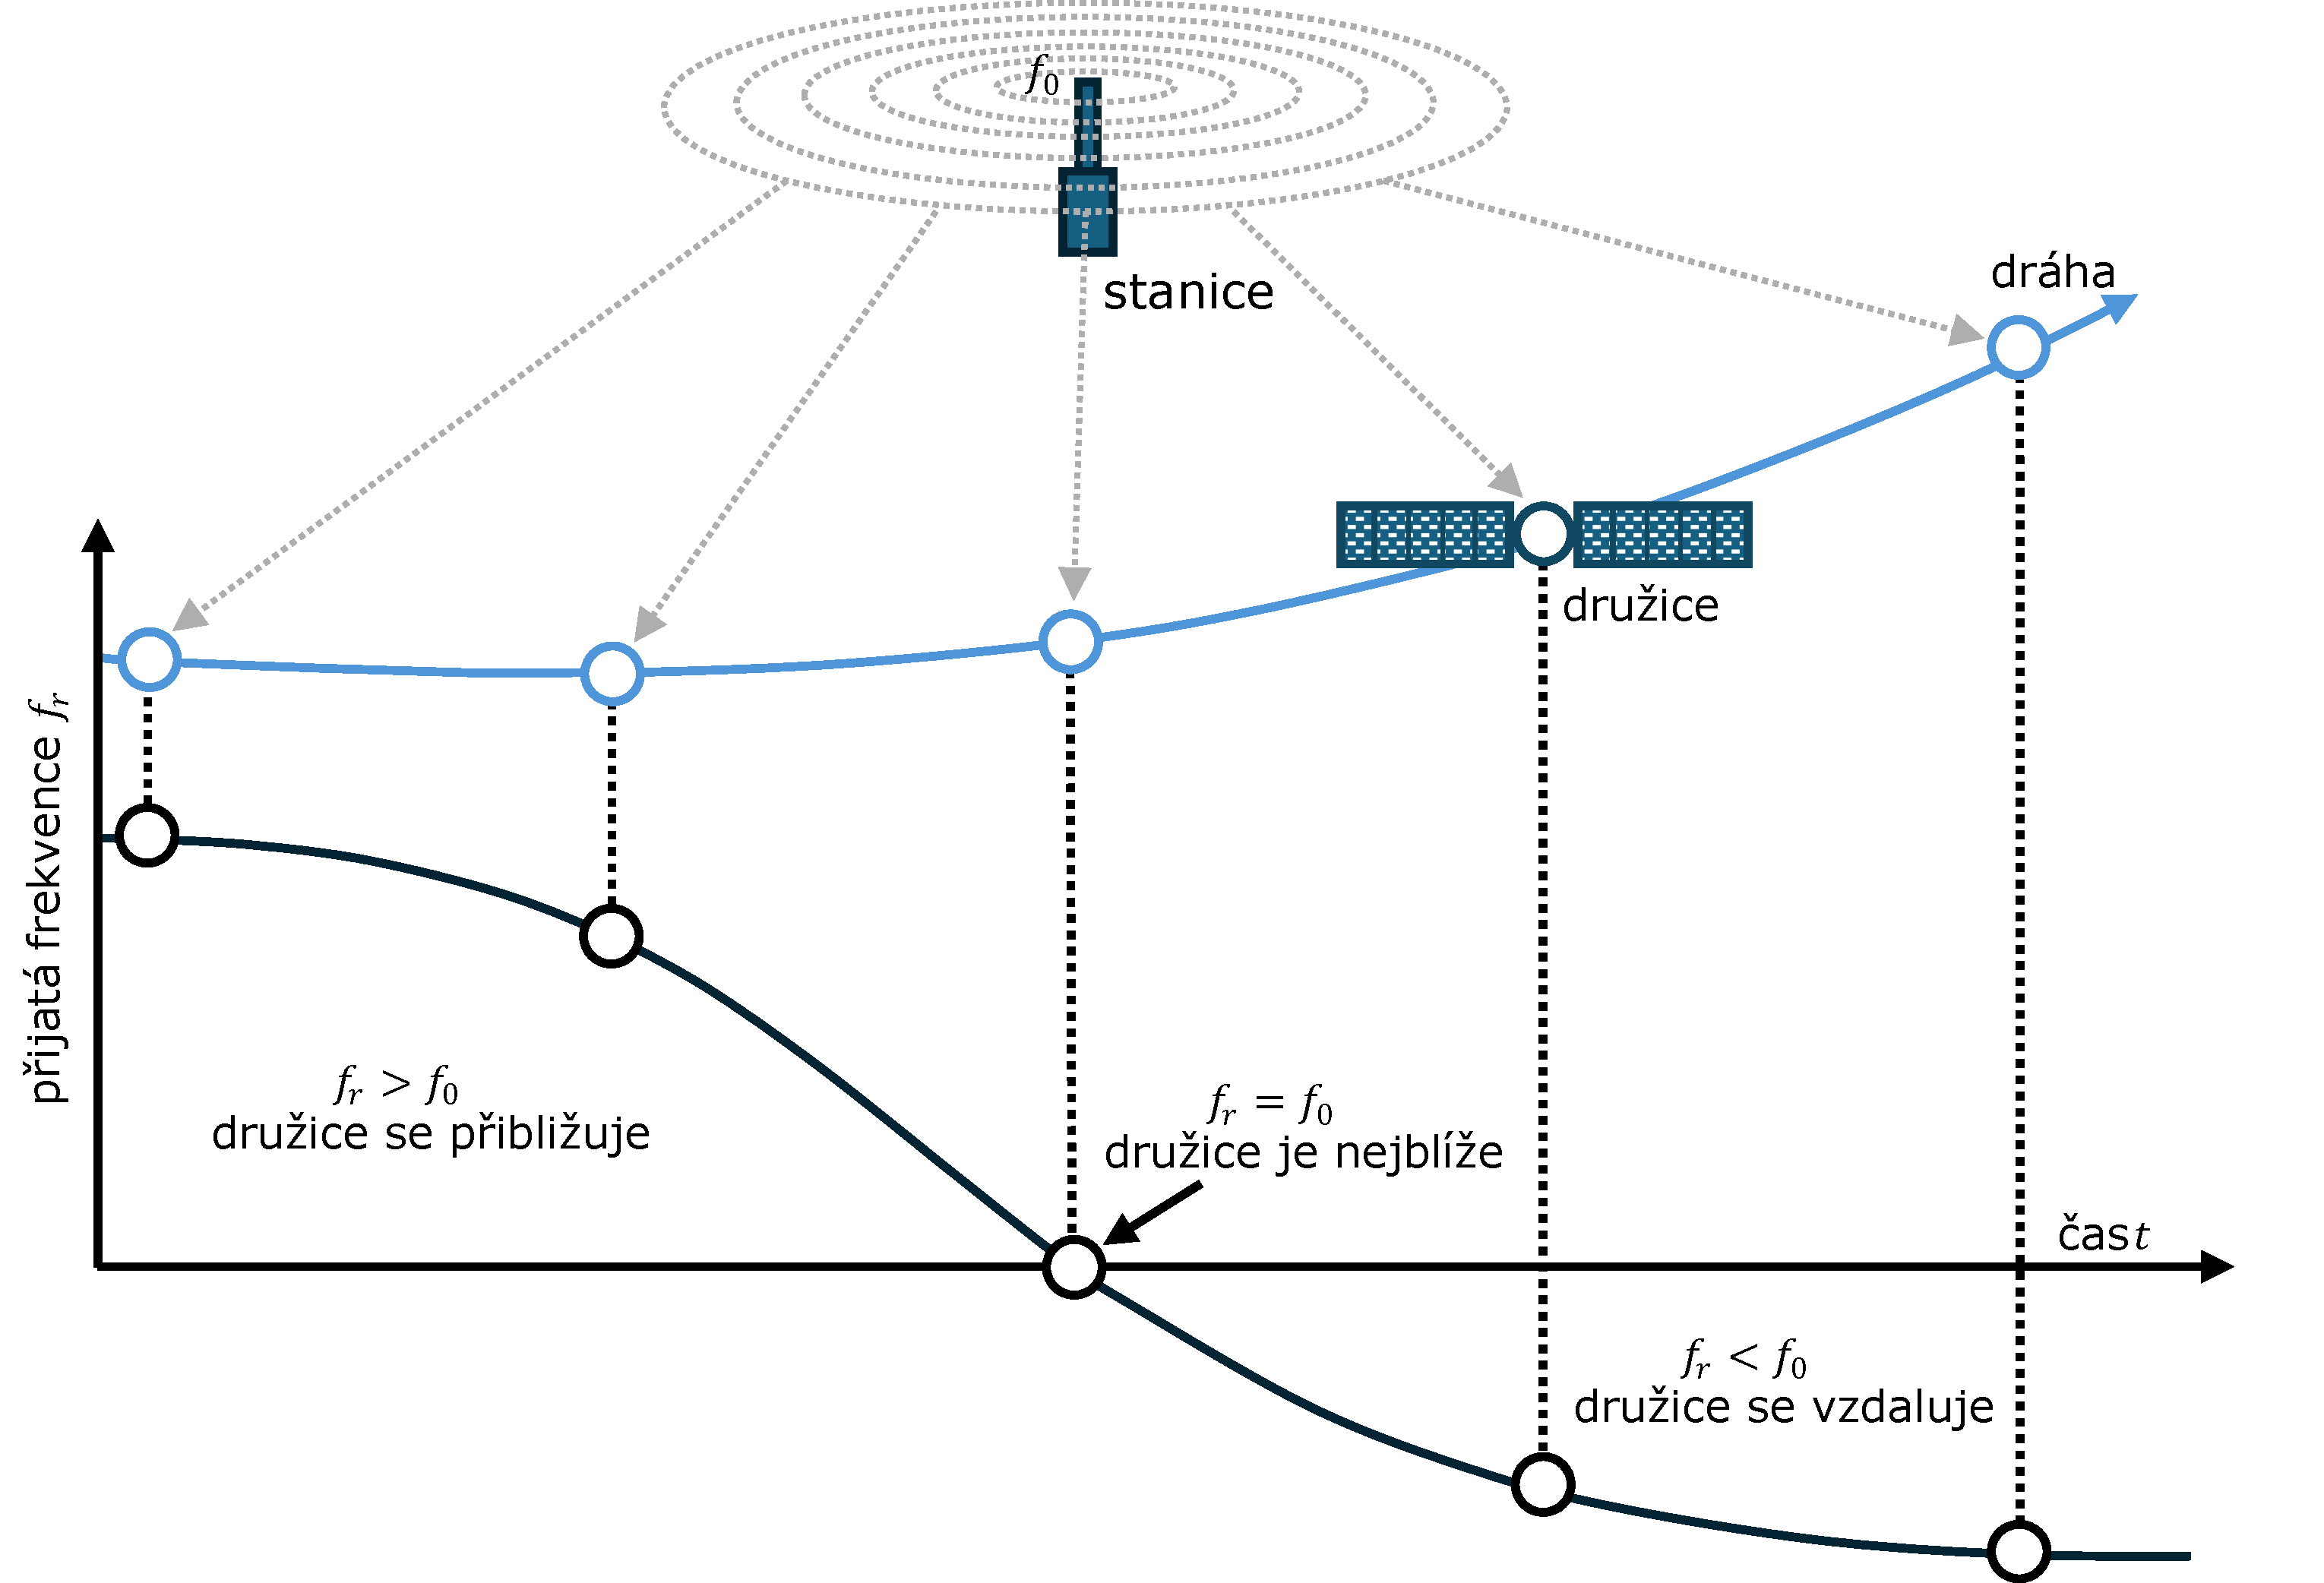
\includegraphics[width=1\linewidth]{images/Doris_doppler.pdf}
    \caption{Schéma principu měření systému DORIS (podle~\cite{ggos_doris})}
    \label{fig:doris_system}
\end{figure}

Výhodou uspořádání systému \zkratka{DORIS} je relativní konstrukční jednoduchost palubního přijímače, jeho nižší energetická náročnost a menší prostorové požadavky. Díky tomu může být systém \zkratka{DORIS} integrován i na družice, jejichž primární mise není geodetická, ale například altimetrická, oceánografická, zaměřená na studium kryosféry nebo na dálkový průzkum Země.

\subsection{Struktura IDS}

\zkratka{IDS} je mezinárodní služba působící v~rámci organizací \zkratka{IAG} a \zkratka{GGOS}. Jejím hlavním cílem je koordinace zpracování dat systému \zkratka{DORIS} a publikace oficiálních produktů. \zkratka{IDS} se skládá z~několika složek (viz obr.~\ref{fig:ids_structure})~\cite{ggos_ids}. Nejvyšším orgánem je Governing Board, který určuje strategii rozvoje služby, schvaluje standardy a koordinuje spolupráci s~ostatními geodetickými službami. Organizační a komunikační činnost zajišťuje Central Bureau, které spravuje dokumentaci, technické standardy a organizuje odborná setkání. Datová centra (Data Centers) slouží k~archivaci a distribuci surových i zpracovaných dat, včetně měření ve formátu \texttt{RINEX}, řešení analytických center a kombinovaných produktů. Analytická centra (Analysis Centers) nezávisle zpracovávají data systému \zkratka{DORIS} a poskytují řešení drah družic, souřadnic stanic a parametrů orientace Země. Mezi významná analytická centra patří například CNES/\allowbreak CLS, IGN, NASA/\allowbreak GSFC nebo ESOC, přičemž důležitým přispěvatelem je také Geodetická observatoř Pecný (\zk{GOP}). Výsledná nezávislá řešení jednotlivých analytických center jsou následně slučována do jednoho oficiálního řešení \zkratka{IDS} v~rámci kombinačního centra (Combination Center), které vytváří oficiální produkty \zkratka{IDS}~\cite{ids_structure}.

\begin{figure}[H]
    \centering
    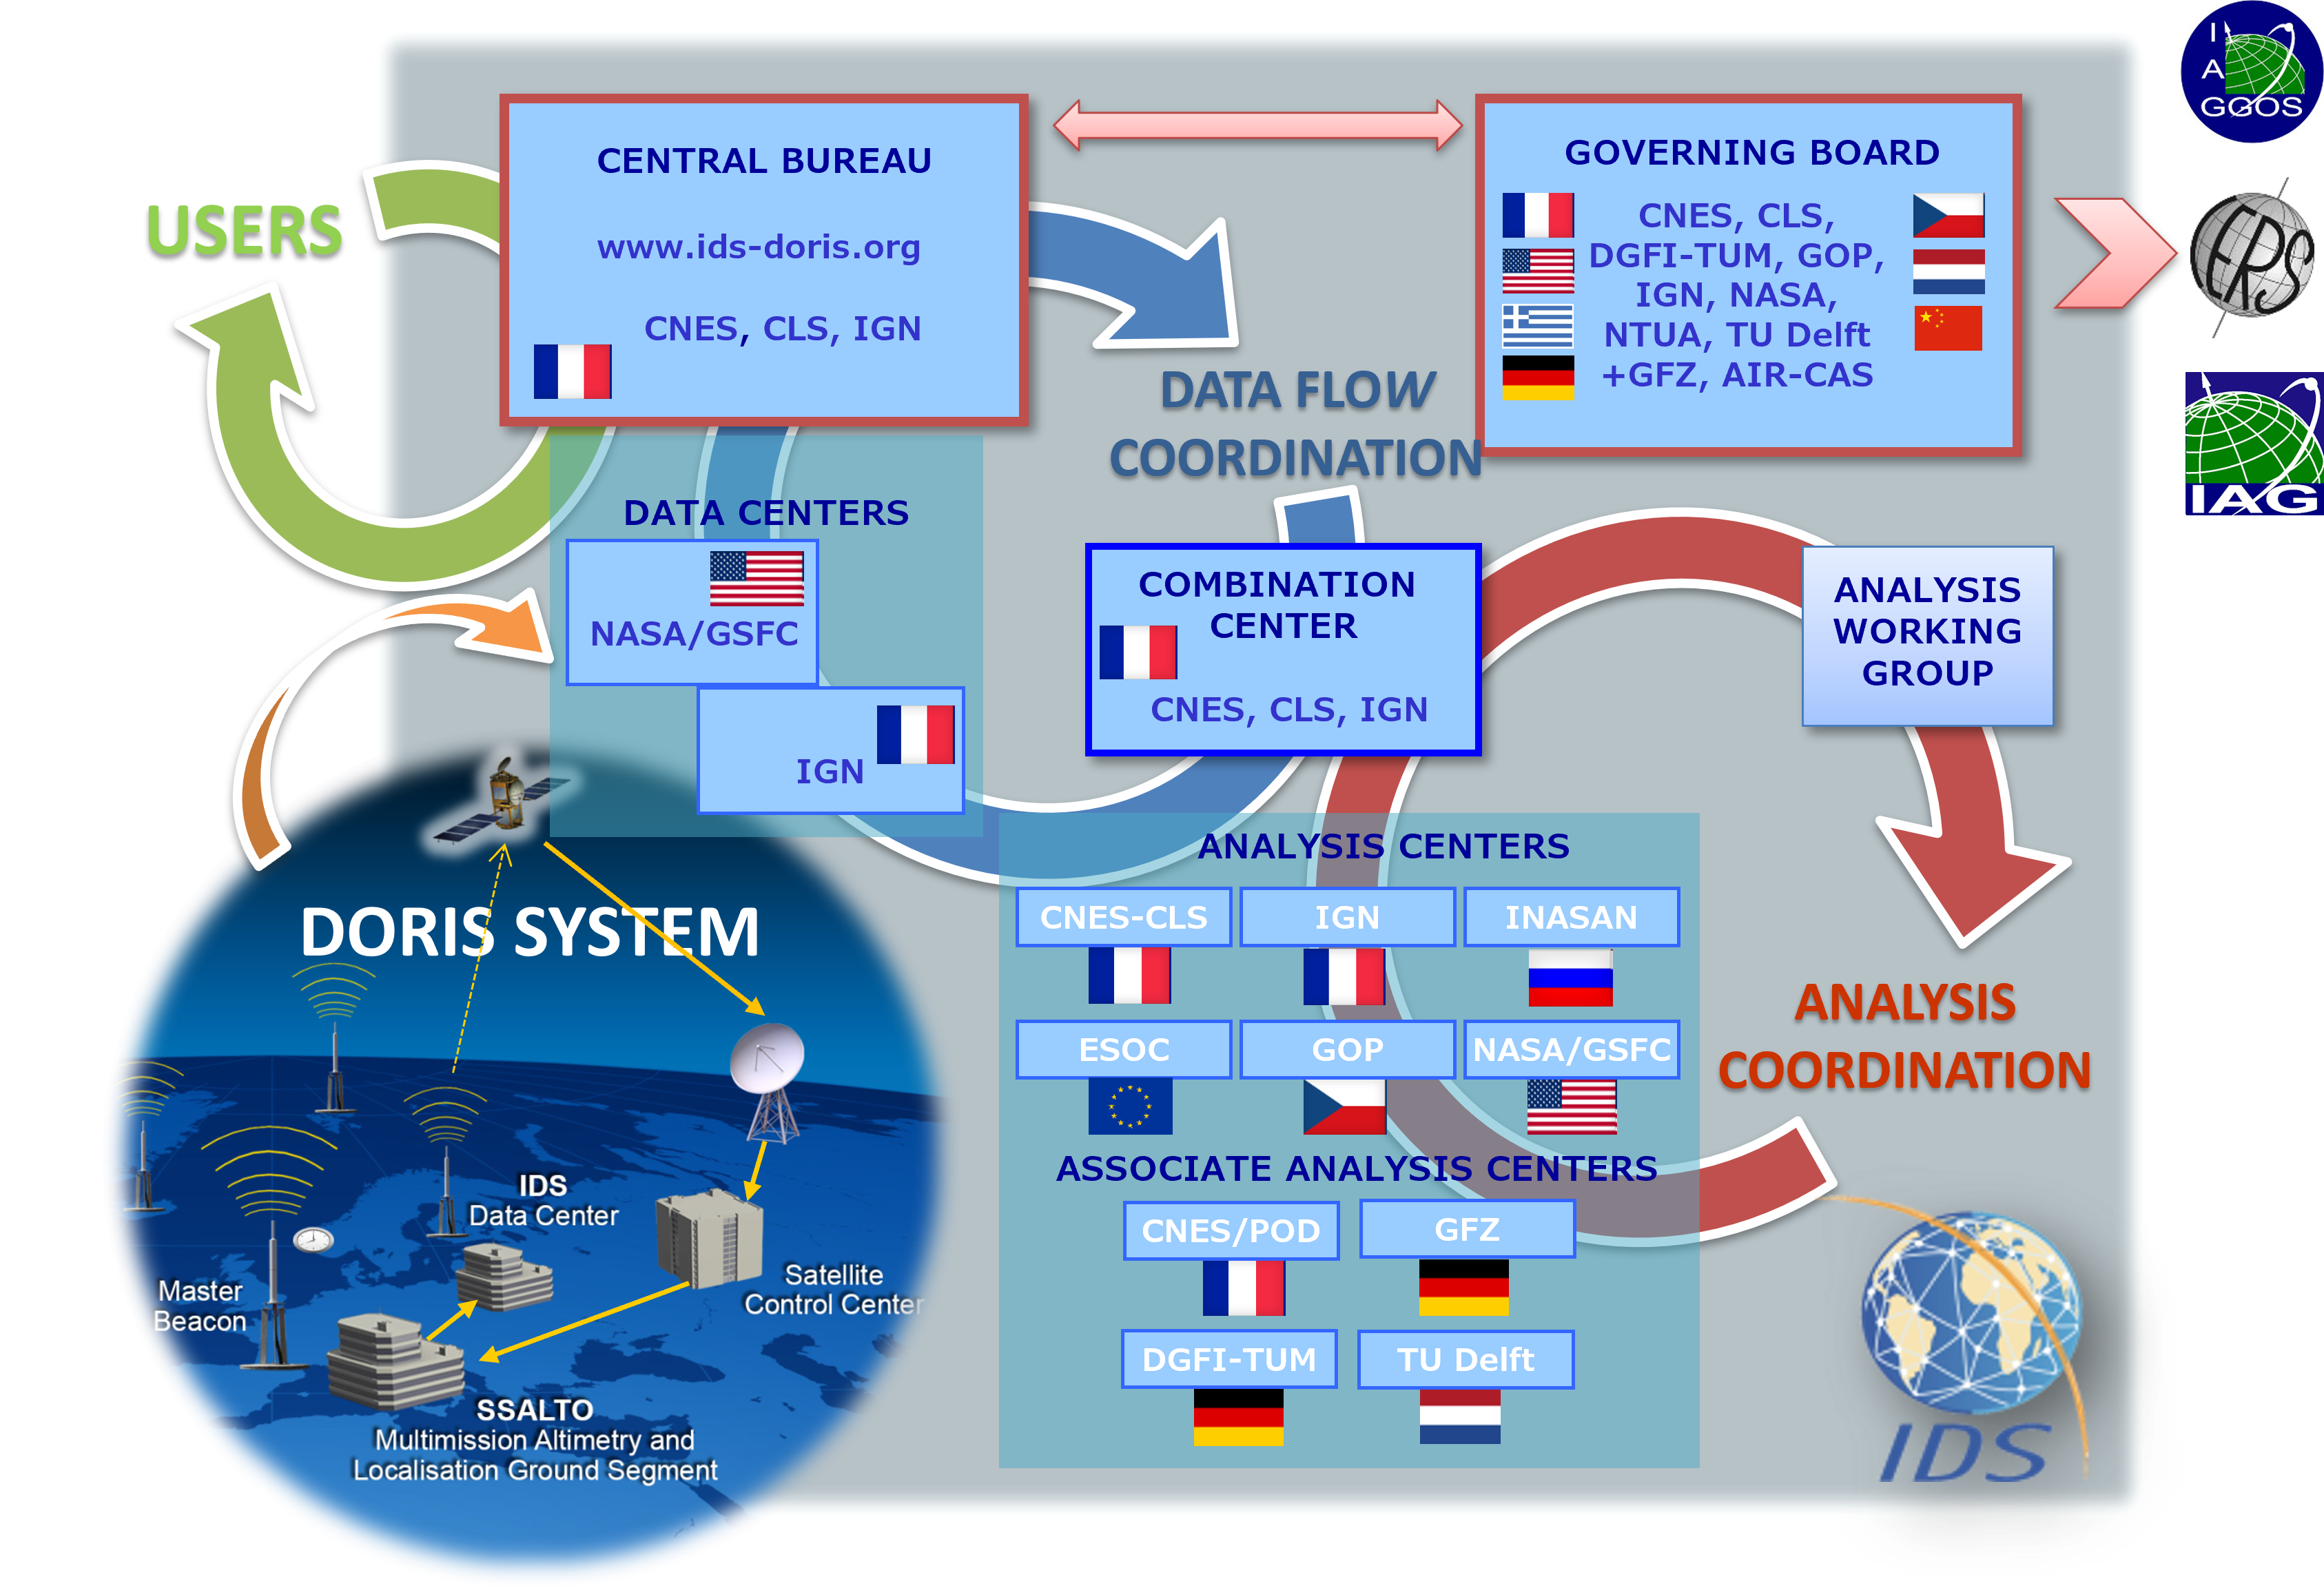
\includegraphics[width=0.9\linewidth]{images/Struktura_ids.png}
    \caption{Struktura služby IDS (převzato z~\cite{ids_structure})}
    \label{fig:ids_structure}
\end{figure}

\subsection{Přínos systému DORIS}

Produkty služby \zkratka{IDS} jsou využívány k~mnoha aplikacím v~oblasti geodézie a \mbox{geodynamiky}. Systém \zkratka{DORIS} slouží především pro přesné určování drah družic, které jsou nezbytné například pro altimetrické mise a dálkový průzkum Země. Kromě toho umožňuje určování souřadnic a rychlostí pozemních stanic, stanovení parametrů orientace Země a sledování změn polohy geocentra~\cite{moreaux_2023_itrf2020}. Díky dlouhodobým časovým řadám souřadnic stanic lze data systému \zkratka{DORIS} využít také pro studium geodynamických procesů, jako jsou pohyby tektonických desek nebo deformace zemské kůry. Systém \zkratka{DORIS} patří vedle dalších technik kosmické geodézie, jako jsou \zkratka{GNSS}, \zkratka{SLR} a \zkratka{VLBI}, mezi klíčové zdroje dat využívané při realizaci \mbox{mezinárodního} terestrického referenčního rámce (\zk{ITRF}). Přínos služby \zkratka{IDS} k~realizaci \zk{ITRF}2020 je podrobně popsán například v~práci Moreaux et al.~\cite{moreaux_2023_itrf2020}, která hodnotí kvalitu a stabilitu řešení poskytovaných jednotlivými analytickými centry. Na úrovni konkrétních řešení se problematikou zpracování dat systému \zkratka{DORIS} zabývají také Štěpánek et al.~\cite{stepanek_2023_gop_itrf2020,stepanek_2006_doris_data_analysis}, kteří popisují přístup Geodetické observatoře Pecný a její příspěvek k~mezinárodním kombinacím. Dále Schreiner et al.~\cite{schreiner_2023_pod_doris_gps_slr} ukazují, že kombinace technik \zkratka{DORIS}, \zkratka{GPS} a~\zkratka{SLR} vede ke~zvýšení přesnosti drah u~misí Sentinel-3 a~Sentinel-6.

\section{Základní informace o~časových řadách}

Analýza časových řad souřadnic geodetických stanic je standardně využívána pro hodnocení stability geodetických sítí a kvality zpracování dat. Z~toho důvodu je problematika časových řad souřadnic stanic v~literatuře podrobně zpracována. V~případě stanic systému \zkratka{DORIS} mají tyto analýzy význam také pro hodnocení konzistence řešení poskytovaných jednotlivými analytickými centry \zkratka{IDS}, jejichž kombinací vzniká oficiální řešení~\cite{moreaux_2023_itrf2020}. Časové řady jsou obvykle modelovány jako kombinace trendu, periodických složek a případných diskontinuit, které mohou vznikat například v~důsledku změn ve zpracování, v~měření nebo geofyzikálních jevů. Přehled metod analýzy těchto časových řad poskytují například Bos et al.~\cite{bos_2019_time_series}, kteří popisují tzv. trajectory model zahrnující uvedené složky.

Dlouhodobý trend časové řady je nejčastěji odhadován metodou nejmenších čtverců, jejíž teoretické základy jsou detailně vysvětleny například v~publikaci \mbox{Montgomery} et al.~\cite{montgomery_regression}. V~praxi je přitom nutné zvolit vhodný model trendu. Z~tohoto důvodu je vhodné uvažovat více kandidátních modelů, přičemž pro jejich porovnání lze využít různá informační kritéria, například Bayesovské informační kritérium (\zk{BIC}), které umožňuje zohlednit jak kvalitu aproximace, tak složitost modelu~\cite{kass_raftery_1995}.

Pro analýzu periodických složek časových řad se využívá spektrální analýza. Mezi nejběžnější metody spektrální analýzy patří zejména rychlá Fourierova trans\-formace (\zk{FFT})~\cite{cooley_tukey_1965} a Lomb--Scargleův periodogram, který je vhodný pro nepravidelně vzorkovaná data~\cite{lomb_scargle}.

Detekce zlomů umožňuje identifikovat změny statistických vlastností časových řad. Přehled metod pro detekci zlomů uvádí například Truong et al.~\cite{change_point_review}.

Popis šumu, tedy náhodné složky dat, je rozebrán v~práci Bos et al.~\cite{bos_2019_time_series}. Šum v~časových řadách obvykle není čistě bílý, ale vykazuje časovou závislost, a proto je často modelován jako kombinace více typů šumu.

\section{Základní informace o~drahách družic}

Přesné určování drah družic je jednou z~klíčových úloh v~oblasti kosmické geodézie a dálkového průzkumu Země. Přesnost určení dráhy má zásadní vliv na kvalitu výsledků altimetrických měření, navigačních aplikací i geodetických produktů.

Pro dosažení vyšší přesnosti bývají využívány kombinace různých technik kosmické geodézie, mezi které patří například \zkratka{DORIS}, \zkratka{GPS} a \zkratka{SLR}. Problematikou přesného určování drah družic pomocí kombinace těchto technik se zabývají například Schreiner et al.~\cite{schreiner_2023_pod_doris_gps_slr}, kteří analyzují řešení drah družic Sentinel-3A/B a Sentinel-6A. Kombinací metod \zkratka{SLR} a \zkratka{DORIS} se zabývá také práce Zeitlhöfler et al.~\cite{zeitlhoefler_2025_combined_orbit_slr_doris}.

Pro zhodnocení konzistence jednotlivých řešení drah družic se provádí jejich vzájemné porovnání na základě rozdílů polohy družice mezi jednotlivými řešeními. Rozdíly drah družic jsou vyjadřovány buď v~kartézském souřadnicovém systému, nebo v~lokálním orbitálním referenčním systému \zkratka{RTN}, který umožňuje fyzikální interpretaci odchylek~\cite{schreiner_2023_pod_doris_gps_slr}. Pro kvantitativní hodnocení se využívají statistické charakteristiky, zejména kvadratická odchylka (RMS)~\cite{stepanek_2023_gop_itrf2020}.

Vzhledem k~tomu, že data nejsou vždy poskytována ve stejné časové škále a nejsou vzorkována ve stejných epochách, je nutné je převést na jednotnou časovou osu a případně interpolovat na společné epochy. Konkrétní interpolační metody jsou podrobně rozebrány v~\cite{zeitlhoefler_2024_interpolation}, kde jsou porovnávány různé přístupy. Jedním z~nich je Hermitova interpolace, která je výhodná, jelikož kromě polohy využívá i rychlost družice, tedy první derivaci dráhy.

\section{Shrnutí současného stavu}

Z~rešerše vyplývá, že jednotlivá témata jako systém \zk{DORIS}, dráhy družic a analýza časových řad jsou dobře popsána. Nebyla však nalezena práce, která by se komplexně zabývala současně analýzou časových řad souřadnic stanic systému \zk{DORIS} a zároveň porovnáním přesných drah družic z~různých analytických center \zkratka{IDS}. Přesto lze z~existujících metod a postupů vycházet a vhodně je kombinovat pro účely této práce.
\chapter{Teorie -- Časové řady}
\label{3-teorie-casove-rady}

Časové řady jsou posloupnosti hodnot měřené veličiny uspořádané podle času. Časové kroky jsou diskrétní a mohou být pravidelně nebo nepravidelně vzorkované. Měřenou veličinou může být skalární hodnota i vektor. V~geodetických aplikacích se časové řady využívají především pro popis změn souřadnic bodů v~čase. Časové řady souřadnic stanic systému \zkratka{DORIS} poskytované v~produktech \zkratka{IDS} obsahují odchylky (dN, dE, dU) vůči apriorním souřadnicím stanice (North, East, Up) a odhady nejistot těchto odchylek (sN, sE, sU). Obecně lze časovou řadu jedné složky \(y(t)\) modelovat jako kombinaci deterministických a stochastických složek~\cite{bos_2019_time_series}:

\begin{equation}
y(t) = T(t) + D(t) + P(t) + \varepsilon(t),
\end{equation}
kde jednotlivé členy představují:

\begin{enumerate}
    \item \textbf{Dlouhodobý trend \(T(t)\)}  
    Lineární nebo nelineární změna souřadnic v~čase, zpravidla interpretovaná jako rychlost pohybu stanice, způsobená například pohybem litosférických desek.

    \item \textbf{Diskontinuity \(D(t)\)}  
    Náhlé změny (skoky) nebo změny trendu v~časové řadě, způsobené například výměnou přístroje, zemětřesením nebo změnou zpracování.

    \item \textbf{Periodická složka \(P(t)\)}  
    Sezónní variace souřadnic, typicky s~roční a půlroční periodou, způsobené například hydrologií nebo teplotními změnami.

    \item \textbf{Náhodná složka \(\varepsilon(t)\)}  
    Šumová složka reprezentující nemodelované procesy a chyby měření.
\end{enumerate}

Cílem analýzy časových řad je zejména:

\begin{enumerate}
    \item odhadnout dlouhodobý trend a jeho případné změny,
    \item identifikovat a kvantifikovat diskontinuity,
    \item určit dominantní periodicity.
\end{enumerate}

\section{Lineární trend}

Lineární trend je základní model dlouhodobého chování časové řady souřadnic. V~geodetických aplikacích je běžně využíván pro odhad rychlosti pohybu stanice. Pro pozorování \(y_i\) v~čase \(t_i\) se uvažuje model
\begin{equation}
y_i = a + b\,t_i + \varepsilon_i,
\label{eq:lin_model}
\end{equation}
kde
\begin{itemize}
    \item \(a\) je absolutní člen,
    \item \(b\) je směrnice přímky vyjadřující rychlost změny v~čase (např. v~mm/rok),
    \item \(\varepsilon_i\) je náhodná zbytková složka.
\end{itemize}
Model lze zapsat maticově jako
\begin{equation}
\mathbf{y}=\mathbf{X}\boldsymbol{\beta}+\boldsymbol{\varepsilon},
\end{equation}
kde platí
\[
\mathbf{y}=\begin{bmatrix}y_1\\y_2\\\vdots\\y_n\end{bmatrix},\quad
\mathbf{X}=\begin{bmatrix}1&t_1\\1&t_2\\\vdots&\vdots\\1&t_n\end{bmatrix},\quad
\boldsymbol{\beta}=\begin{bmatrix}a\\b\end{bmatrix},\quad
\boldsymbol{\varepsilon}=\begin{bmatrix}\varepsilon_1\\\varepsilon_2\\\vdots\\\varepsilon_n\end{bmatrix}.
\]

\paragraph{Odhad parametrů metodou nejmenších čtverců}\leavevmode\\
Parametry \((a,b)\) se odhadují metodou nejmenších čtverců, která je založena na minimalizaci součtu čtverců reziduí. Pro jednotlivá pozorování to lze zapsat jako
\begin{equation}
RSS = \sum_{i=1}^{n} p_i \left(y_i - a - b\,t_i\right)^2 \rightarrow \min,
\label{eq:lsq_min}
\end{equation}
kde \(p_i\) jsou váhy jednotlivých pozorování, často volené například jako \(p_i = 1/\sigma_i^2\).

\noindent RSS lze v~maticovém zápisu zapsat jako
\begin{equation}
RSS = \mathbf{e}^\mathrm{T}\mathbf{P}\mathbf{e} \rightarrow \min,
\label{eq:lsq_matrix}
\end{equation}
kde \(\mathbf{e} = \mathbf{y} - \mathbf{X}\boldsymbol{\beta}\) je vektor reziduí
a \(\mathbf{P} = \mathrm{diag}(p_1,\dots,p_n)\) je diagonální matice vah.
Odhad parametrů je dán vztahem
\begin{equation}
\hat{\boldsymbol{\beta}} = (\mathbf{X}^\mathrm{T}\mathbf{P}\mathbf{X})^{-1}\mathbf{X}^\mathrm{T}\mathbf{P}\mathbf{y}.
\end{equation}
Vyrovnané hodnoty a rezidua jsou dány vztahy:
\begin{equation}
\hat{y}_i=\hat{a}+\hat{b}\,t_i,\qquad
e_i=y_i-\hat{y}_i.
\label{eq:residuals}
\end{equation}
Koeficient determinace \(R^2\) vyjadřuje podíl variability vysvětlené modelem:
\begin{equation}
R^2=\frac{\sum_{i=1}^{n}(\hat{y}_i-\bar{y})^2}{\sum_{i=1}^{n}(y_i-\bar{y})^2},
\label{eq:r2}
\end{equation}
kde \(\bar{y} = \frac{1}{n}\sum_{i=1}^{n}y_i\) je průměr pozorování.

\noindent Pro následnou analýzu se často pracuje s~detrendovanou řadou
\begin{equation}
y^{\mathrm{detr}}_i = y_i - \hat{y}_i.
\label{eq:detrend}
\end{equation}

\section{Model s~diskontinuitou}
\label{3-3-mode-s-diskontinuitou}

Jednoduchý lineární trend nemusí zachytit náhlé změny (skoky) nebo změny rychlosti (lom trendu).
Proto je uvažován model se změnou parametrů v~čase \(\tau\):
\begin{equation}
y_i=
\begin{cases}
a_1+b_1\,t_i+\varepsilon_i, & t_i<\tau,\\
a_2+b_2\,t_i+\varepsilon_i, & t_i\geq\tau.
\end{cases}
\label{eq:2seg_model}
\end{equation}
Tento model umožňuje současně popsat skok i změnu sklonu.

\paragraph{Určení polohy lomu}\leavevmode\\
Poloha lomu \(\tau\) není předem známa a určuje se testováním kandidátních hodnot \(\tau\in\mathcal{T}\),
kde \(\mathcal{T}\) je podmnožina pozorovaných časů (krajní hodnoty se obvykle vyloučí).
Pro každé \(\tau\) se odhadnou parametry modelu a spočte se
\begin{equation}
RSS(\tau)=\sum_{i=1}^{n} e_i^2(\tau),
\label{eq:rss_tau}
\end{equation}
kde \(e_i(\tau)\) jsou rezidua pro daný model. Nejvhodnější \(\tau\) odpovídá minimu \(RSS(\tau)\).

\paragraph{Bayesovské informační kritérium (\zk{BIC})}\leavevmode\\
Pro posouzení vhodnosti modelu se používá Bayesovské informační kritérium (\zk{BIC}), které zohledňuje jak kvalitu aproximace, tak složitost modelu~\cite{kass_raftery_1995}:

\begin{equation}
BIC = n\,\ln\!\left(\frac{RSS}{n}\right) + k\,\ln(n),
\label{eq:bic}
\end{equation}
kde \(n\) je počet pozorování a \(k\) počet odhadovaných parametrů. Pro porovnání dvou modelů se sleduje rozdíl
\begin{equation}
\Delta BIC = BIC_{\mathrm{2}}-BIC_{\mathrm{1}},
\label{eq:delta_bic}
\end{equation}
kde \(BIC_1\) odpovídá jednoduššímu modelu a \(BIC_2\) modelu složitějšímu, přičemž \(\Delta BIC < 0\) značí preferenci složitějšího modelu, jelikož zlepšení kvality aproximace převáží penalizace za jeho vyšší složitost. Body zlomu \(\tau\) jsou přidávány iterativně, dokud \(\Delta BIC < 0\).

\section{Detekce diskontinuit}

Diskontinuity v~časových řadách mohou být způsobeny fyzikálními jevy (např. zemětřesení), změnami vysílače, přijímače, nebo artefakty zpracování. Diskontinuity lze určovat buď současně s~odhadem trendu, nebo samostatně, kdy je cílem identifikovat časové okamžiky nestandardního chování řady, případně odhalit diskontinuity, které nebyly při společném odhadu s~trendem zachyceny. Pro samostatnou detekci diskontinuit lze využít například metodu dvou pohyblivých oken nebo přístupy založené na vyhlazení časové řady a následné analýze jejích změn.

\subsection{Metoda dvou pohyblivých oken}

Metoda dvou pohyblivých oken porovnává průměrné hodnoty časové řady ve dvou úsecích dat (oknech) o~stejné délce \(W\), které jsou vůči sobě posunuty o~\(s\) vzorků. Spočteny jsou průměry v~oknech \(\mu_1\) a \(\mu_2\). Kandidát na skok je detekován, pokud platí
\begin{equation}
|\mu_2-\mu_1| > \lambda.
\end{equation}
Volbu prahu \(\lambda\) lze založit na násobku směrodatné odchylky jako heuristiku
\begin{equation}
\lambda = k\,\sigma,
\end{equation}
nebo ji lze odvodit na základě statistického testu rovnosti středních hodnot obou oken (např. dvouvýběrového t-testu), který umožňuje posoudit významnost rozdílu \(\mu_1\) a \(\mu_2\) při zvolené hladině významnosti~\cite{change_point_review}.

\subsection{Vyhlazení a analýza derivace}

Další možností detekce skoků v~časové řadě je potlačení vlivu náhodného šumu pomocí vyhlazení a následná analýza derivace výsledné křivky. Skok se po vyhlazení projeví jako lokálně zvětšená absolutní hodnota derivace. Pro vyhlazení lze využít například metodu LOWESS (Locally Weighted Scatterplot Smoothing), která provádí lokální regresi s~váhami klesajícími se vzdáleností v~čase~\cite{statsmodels_lowess}. Ve vyhlazené časové řadě \( \tilde{y}(t) \) lze derivaci aproximovat mezi sousedními body:
\begin{equation}
v_i \approx \frac{\tilde{y}_{i+1}-\tilde{y}_i}{t_{i+1}-t_i}.
\label{eq:derivative}
\end{equation}
Za kandidáty skoků se považují epochy, kdy \(|v_i|\) překročí zvolený práh. Volbu prahu lze založit na násobku směrodatné odchylky hodnot derivace ve vyhlazené řadě jako heuristiku, případně jej lze odvodit na základě statistického testu (např. pomocí z-testu), který umožňuje posoudit významnost velikosti derivace při zvolené hladině významnosti.

\section{Spektrální analýza}
\label{3-5-spektralni}

Po odstranění trendu a diskontinuit lze časové řady analyzovat z~hlediska periodických složek. Typicky lze očekávat roční a pololetní periodicity související s~geofyzikálními procesy. V~datech se mohou vyskytovat i další periodicity související například s~modelovými chybami. Pro identifikaci periodicit lze využít spektrální analýzu na základě Fourierovy transformace nebo Lomb--Scargleova periodogramu.

\subsection{Fourierova transformace}

Diskrétní Fourierova transformace převádí časovou řadu na frekvenční reprezentaci~\cite{bos_2019_time_series}:
\begin{equation}
Y_k = \sum_{i=0}^{n-1} y_i\, e^{-2\pi \mathrm{i} k~i/n}, \qquad k=0,1,\dots,n-1,
\label{eq:dft}
\end{equation}
kde \(Y_k\) jsou komplexní koeficienty. Každému \(k\) odpovídá frekvence
\begin{equation}
f_k = \frac{k}{n\,\Delta t},
\label{eq:freq}
\end{equation}
kde \(n\) je počet vzorků a \(\Delta t\) interval vzorkování. Pro frekvence \(f_k > 0\) odpovídá perioda vztahu
\begin{equation}
T_k = \frac{1}{f_k}.
\label{eq:period}
\end{equation}

\paragraph{Rychlá Fourierova transformace (FFT)}\leavevmode\\
FFT představuje efektivní algoritmus pro výpočet diskrétní Fourierovy \mbox{transformace} (DFT) s~výpočetní složitostí $\mathcal{O}(n \log n)$~\cite{cooley_tukey_1965}. Pro reálná data se často používá jedno\-stranné spektrum (kladné frekvence), neboť Fourierovo spektrum je pro reálné signály komplexně sdruženě symetrické.

\paragraph{Identifikace dominantních periodicit}\leavevmode\\
Dominantní periodicity se určují vyhledáním lokálních maxim amplitudového spektra. Amplituda vyjadřuje sílu příslušné harmonické složky, fáze pak její časové posunutí. Pro možnost srovnání různých stanic a složek je vhodné časovou řadu před výpočtem spektra standardizovat, například odečtením průměru a vydělením směrodatnou odchylkou.

\subsection{Lomb--Scargleův periodogram}

Lomb--Scargleův periodogram je metoda spektrální analýzy vhodná i pro nepravidelně vzorkovaná data~\cite{lomb_scargle}. Metoda je založena na aproximaci časové řady harmonickou funkcí pomocí metody nejmenších čtverců. Pro každou testovanou frekvenci je časová řada aproximována harmonickou funkcí ve tvaru

\begin{equation}
y(t_i) = A~\cos(\omega t_i) + B \sin(\omega t_i) + \varepsilon_i,
\end{equation}
kde:
\begin{itemize}
    \item \(A\) a \(B\) jsou koeficienty kosinusové a sinusové složky modelu,
    \item \(\omega = 2\pi f\) je úhlová frekvence určující rychlost kmitání harmonické složky,
    \item \(t_i\) jsou časové okamžiky pozorování,
    \item \(y(t_i)\) jsou odpovídající hodnoty časové řady,
    \item \(\varepsilon_i\) je náhodná složka reprezentující šum a nemodelované vlivy.
\end{itemize}

Pro každou úhlovou frekvenci \(\omega\) jsou parametry \(A\) a \(B\) odhadnuty tak, aby byl minimalizován součet čtverců reziduí, tedy aby model co nejlépe aproximoval pozorovaná data. Úhlová frekvence \(\omega\) převádí časovou proměnnou na fázi sinusové funkce a určuje rychlost kmitání harmonické složky. Zatímco frekvence \(f\) udává počet cyklů za jednotku času, úhlová frekvence vyjadřuje rychlost změny fáze sinusové funkce v~radiánech. Hodnota periodogramu pro danou frekvenci je dána vztahem~\cite{lomb_scargle}
\begin{equation}
P(\omega) = \frac{1}{2} \left[
\frac{\left( \sum_{i=1}^{n} y_i \cos(\omega (t_i - \tau)) \right)^2}
{\sum_{i=1}^{n} \cos^2(\omega (t_i - \tau))}
+
\frac{\left( \sum_{i=1}^{n} y_i \sin(\omega (t_i - \tau)) \right)^2}
{\sum_{i=1}^{n} \sin^2(\omega (t_i - \tau))}
\right],
\label{eq:ls_periodogram}
\end{equation}
kde \(\tau\) představuje pomocný časový posun, který je pro každou frekvenci volen tak, aby sinusová a kosinusová složka modelu byly vzájemně ortogonální.

Vysoké hodnoty \(P(\omega)\) odpovídají frekvencím, pro které časová řada obsahuje výraznou periodickou složku.

Na rozdíl od \zk{FFT} je výpočet Lomb--Scargleova periodogramu obecně výpočetně náročnější, protože hodnoty periodogramu jsou určovány samostatně pro každou testovanou frekvenci. Přímý výpočet má proto složitost přibližně $\mathcal{O}(n \cdot m)$, kde \(m\) je počet testovaných frekvencí~\cite{lomb_scargle}.
\chapter{Teorie -- Dráhy družic}
\label{4-teorie-drahy-druzic}

\section{Pohyb družice (Keplerovský pohyb)}

Pohyb družice lze idealizovat jako pohyb v~gravitačním poli Země, kde je Země uvažována jako koule se středově souměrným rozložením hmoty a nejsou uvažovány žádné vnější vlivy. Takto zjednodušený model pohybu se označuje jako Keplerovský pohyb a představuje základní teoretický popis oběžných drah~\cite{bursa_kostelecky_1994}. Gravitační pole ideální Země lze popsat gravitačním potenciálem

\begin{equation}
V~= -\frac{GM}{\rho},
\end{equation}
kde:
\begin{itemize}
    \item $G$ je gravitační konstanta,
    \item $M$ hmotnost Země,
    \item $\rho = |\mathbf{r}|$ vzdálenost družice od středu Země,
    \item $\mathbf r$ je polohový vektor družice vzhledem ke středu Země.
\end{itemize}
Zrychlení družice v~potenciálovém poli je dáno záporným gradientem potenciálu

\begin{equation}
\ddot{\mathbf r} = - \nabla V.
\end{equation}
Pro potenciál gravitačního pole ideální Země pak platí

\begin{equation}
\nabla V~= \frac{GM}{\rho^3}\mathbf r,
\end{equation}
a výsledná rovnice pohybu má tvar

\begin{equation}
\ddot{\mathbf r} = -\frac{GM}{\rho^3}\mathbf r.
\end{equation}

Tuto rovnici lze rozložit jako soustavu tří diferenciálních rovnic druhého řádu, která při zadaných počátečních podmínkách (poloze a rychlosti), jednoznačně určuje pohyb družice. Z~jejího tvaru je zřejmé, že zrychlení je v~každém okamžiku orientováno do středu Země, a pohyb tedy probíhá v~centrálním silovém poli. V~centrálním silovém poli je zachován moment hybnosti družice

\begin{equation}
\mathbf h = \mathbf r \times \dot{\mathbf r},
\end{equation}
z~čehož plyne, že pohyb probíhá v~jedné rovině a že plošná rychlost průvodiče je konstantní. Tato vlastnost odpovídá druhému Keplerovu zákonu~\cite{bursa_kostelecky_1994}.

Řešením rovnice pohybu v~centrálním gravitačním poli jsou kuželosečky. V~případě umělých družic Země se jedná především o~eliptické dráhy, které lze popsat vztahem

\begin{equation}
\rho = \frac{a(1 - e^2)}{1 + e \cos \nu},
\end{equation}

kde 
\begin{itemize}
    \item $a$ je hlavní poloosa, 
    \item $e$ je excentricita,
    \item $\nu$ je pravá anomálie.
\end{itemize}

Keplerovy zákony popisují geometrické vlastnosti dráhy i časový průběh pohybu. V~tomto smyslu nepředstavují samostatný předpoklad, ale důsledek pohybu v~centrálním gravitačním poli.

Polohu a orientaci eliptické dráhy lze jednoznačně popsat pomocí šesti Keplerovských elementů: hlavní poloosy $a$, excentricity $e$, sklonu dráhy $i$, rektascenze vzestupného uzlu $\Omega$, argumentu perigea $\omega$ a střední anomálie $M$. Tyto parametry představují alternativní popis dráhy vůči kartézské poloze a rychlosti a v~případě Keplerovského pohybu jsou konstantní v~čase.

Keplerovský pohyb představuje ideální řešení problému dvou těles. Ve skutečnosti je však pohyb družice ovlivněn řadou dalších sil, které vedou k~odchylkám od ideální eliptické dráhy a ke změnám Keplerovských elementů v~čase. Tím vzniká potřeba uvažovat obecnější, rušený pohyb družice.

\section{Rušený pohyb družice}

Ve skutečnosti se družice nepohybují v~ideálním centrálním gravitačním poli, protože Země není homogenní koule a na družice současně působí další gravitační i negravi\-tační vlivy. Tyto vlivy způsobují odchylky od ideálního Keplerovského pohybu a takový pohyb se označuje jako rušený pohyb družice~\cite{bursa_kostelecky_1994}. Pohyb družice proto nelze popsat pouze Keplerovským modelem, ale je nutné uvažovat obecnější rovnici pohybu ve tvaru

\begin{equation}
\ddot{\mathbf{r}} = -\frac{GM}{\rho^3}\mathbf{r} + \mathbf{a}_{\text{pert}},
\end{equation}
kde 
\begin{itemize}
    \item $\mathbf{a}_{\text{pert}}$ představuje součet poruchových zrychlení.
\end{itemize}
Poruchová zrychlení \(\mathbf{a_{pert}}\) lze rozdělit na gravitační a negravitační. 

\paragraph{Mezi gravitační poruchy patří:}
\begin{itemize}
\item nesférické gravitační pole Země popsané harmonickým rozvojem,
\item časově proměnné slapové deformace Země,
\item gravitační působení Slunce, Měsíce a planet.
\end{itemize}

\paragraph{Mezi negravitační poruchy patří:}
\begin{itemize}
\item tlak slunečního záření,
\item záření Země (albedo a infračervené vyzařování),
\item atmosférický odpor (významný zejména pro nízké oběžné dráhy).
\end{itemize}

\section{Přesné určení drah družic}

Přesné určení drah družic (POD) je proces, při němž se na základě měření a dynamického modelu pohybu odhaduje dráha družic. Dynamický model zahrnuje nejen ideální centrální gravitační pole Země, ale i jeho odchylky a další gravitační i negravitační rušivé vlivy.  Odhad dráhy je prováděn nepřímo prostřednictvím odhadu parametrů tohoto modelu, přičemž samotná trajektorie je výsledkem řešení rovnice pohybu. Cílem je určit polohu a rychlost družice v~čase s~co nejvyšší přesností. Výsledkem tohoto procesu jsou produkty přesných drah, typicky poskytované ve formátu SP3, které obsahují diskrétní hodnoty polohy a případně rychlosti družice v~čase.

V~případě systému DORIS je určování dráhy založeno na měření Dopplerova posunu signálu vysílaného pozemními stanicemi a přijímaného na palubě družice. Měřený Dopplerův posun souvisí se změnou vzdálenosti mezi družicí a stanicí v~čase, tedy s~relativní rychlostí ve směru spojnice družice--stanice. Z~časového průběhu těchto měření během průletů družice nad stanicemi lze následně odhadovat parametry  dynamického modelu tak, aby výsledná dráha co nejlépe odpovídala pozorováním~\cite{ids_what_is_doris}.

\section{Dynamická parametrizace dráhy}

Dynamická parametrizace dráhy je způsob modelování drah družic, při kterém je dráha popsána jako řešení rovnice pohybu s~uvažováním gravitačních i negravitačních sil. Na rozdíl od čistě geometrických metod je tento přístup založen na fyzikálním modelu pohybu družice. Dráha družice je obvykle popisována na časově omezených úsecích, tzv. obloucích, v~jejichž rámci jsou aplikovány fyzikální modely a současně odhadovány parametry popisující její pohyb. Tyto parametry určují konkrétní řešení rovnice pohybu. Princip spočívá v~tom, že odhadované parametry jsou voleny tak, aby výsledná trajektorie co nejlépe odpovídala vstupním datům, například diskrétním souřadnicím družice ve formátu SP3~\cite{bernese_5_2}. V~rámci jednoho oblouku jsou aplikovány zejména následující fyzikální modely:

\begin{itemize}

\item \textbf{Gravitační modely}
\begin{itemize}
\item Nesférické gravitační pole Země, popsané pomocí harmonického rozvoje
\item Slapové jevy
\item Gravitační působení Slunce, Měsíce a blízkých planet
\end{itemize}

\item \textbf{Modely negravitačních sil}
\begin{itemize}
\item Apriorní model hustoty atmosféry MSIS-86
\item Apriorní model tlaku slunečního záření
\item Záření odražené a vyzařované Zemí (albedo a infračervené záření)
\end{itemize}

\end{itemize}

\noindent Současně jsou v~rámci jednotlivých oblouků odhadovány následující parametry:

\begin{itemize}

\item \textbf{Počáteční podmínky}
\begin{itemize}
\item Šest parametrů určujících stav družice v~epoše na začátku oblouku. Tyto parametry lze vyjádřit jako polohový vektor a vektor rychlosti, nebo ekvivalentně šesti Keplerovskými elementy.
\end{itemize}

\item \textbf{Odhadované parametry negravitačních sil}
\begin{itemize}
\item Měřítkový koeficient atmosférického odporu
\item Měřítkový koeficient tlaku slunečního záření
\end{itemize}

\item \textbf{Empirické parametry}
Jsou parametry, které nemají jasný fyzikální význam, ale zachycují nemodelované nebo nepřesně modelované vlivy. Mají periodu přibližně odpovídající oběžné době družice. Tyto parametry jsou obvykle definovány ve směrech:
\begin{itemize}
\item R -- radiální (ve směru polohového vektoru),
\item T -- transverzální (ve směru pohybu družice),
\item N -- normálový (kolmo na rovinu dráhy),
\end{itemize}
a jsou vyjádřeny pomocí amplitudy a fáze (sinusové a kosinusové členy). Jejich úlohou je absorbovat zbytkové chyby modelování~\cite{stepanek_2023_gop_itrf2020}.

\end{itemize}

\section{Interpolace drah}

Kromě dynamické parametrizace dráhy z~diskrétních bodů lze pro určení polohy družice v~konkrétní epoše využít také interpolaci mezi známými body, která je čistě matematickým přístupem a nevyžaduje zahrnutí fyzikálních vlivů do výpočtu. Pohyb družice po oběžné dráze je nelineární, a proto je při požadavku na vysokou přesnost vhodné použít interpolační metodu, která kromě polohy zohledňuje také první derivaci polohy, tedy rychlost družice~\cite{zeitlhoefler_2024_interpolation}.

\paragraph{Hermitova interpolace}\leavevmode\\
Hermitova interpolace v~uzlech respektuje nejen hodnotu funkce $f(t)$, ale i její první derivaci $f'(t)$. V~případě drah družic představuje funkce $f(t)$ polohu družice $\mathbf r(t)$ a její derivace $f'(t)$ odpovídá rychlosti družice $\mathbf v(t)=\dot{\mathbf r}(t)$. Jsou dány uzly \(t_0, t_1, \dots, t_n\), v~nichž jsou známy hodnoty $f(t_k)$ a $f'(t_k)$. Hermitův interpolační polynom má stupeň nejvýše $2n+1$~\cite{zeitlhoefler_2024_interpolation}. V~obecném tvaru lze Hermitovu interpolaci zapsat jako:

\begin{equation}
H_{2n+1}(t) = \sum_{k=0}^{n} f(t_k)\,H_{n,k}(t) + \sum_{k=0}^{n} f'(t_k)\,\hat H_{n,k}(t).
\label{eq:hermite_general}
\end{equation}

\paragraph{Lagrangeovy bázové funkce}\leavevmode\\
Základem konstrukce Hermitova interpolačního polynomu jsou Lagrangeovy bázové funkce:

\begin{equation}
L_{n,k}(t)=
\prod_{\substack{i=0 \\ i\neq k}}^{n}
\frac{t-t_i}{t_k-t_i}.
\label{eq:lagrange_basis}
\end{equation}
Pro sestavení Hermitových bázových funkcí je dále potřeba derivace Lagrangeovy bázové funkce v~jejím vlastním uzlu, která je dána vztahem

\begin{equation}
L'_{n,k}(t_k)=
\sum_{\substack{m=0 \\ m\neq k}}^{n}
\frac{1}{t_k-t_m}.
\label{eq:lagrange_deriv}
\end{equation}

\paragraph{Hermitovy báze}\leavevmode\\
Pro danou epochu $t^\ast$

\begin{equation}
\Delta t_k = t^\ast - t_k.
\end{equation}
Hermitovy bázové funkce mají tvar

\begin{equation}
H_{n,k}(t^\ast)
=
\left(
1 - 2 \Delta t_k L'_{n,k}(t_k)
\right)
L_{n,k}^2(t^\ast),
\end{equation}

\begin{equation}
\hat H_{n,k}(t^\ast)
=
\Delta t_k
L_{n,k}^2(t^\ast).
\end{equation}
Funkce $H_{n,k}$ váží příspěvek polohy v~uzlu $t_k$,
zatímco $\hat H_{n,k}$ váží příspěvek rychlosti.

\paragraph{Výsledný tvar}

Interpolovaná poloha družice v~epoše $t^\ast$ je určena vztahem

\begin{equation}
\mathbf r(t^\ast)
=
\sum_{k=0}^{n}
\mathbf r(t_k)\, H_{n,k}(t^\ast)
+
\sum_{k=0}^{n}
\mathbf v(t_k)\, \hat H_{n,k}(t^\ast).
\end{equation}
kde:
\begin{itemize}
    \item \(\mathbf{r}\) je polohový vektor \((x, y, z)\)
    \item \(\mathbf{v}\) je vektor rychlosti \((v_x, v_y, v_z)\)
\end{itemize}

Interpolace je prováděna složkově pro jednotlivé kartézské souřadnice, přičemž bázové funkce jsou společné pro všechny složky vektoru. Interpolační polynom je obvykle konstruován na základě uzlů z~okolí požadované epochy.

\section{Transformace rozdílů do systému RTN}

Pro interpretaci rozdílů drah se často používá lokální orbitální souřadnicový systém RTN~\cite{zeitlhoefler_2024_interpolation}. Ten tvoří tři na sebe kolmé složky:

\begin{itemize}
\item R – radiální směr (směr polohového vektoru, od středu Země k~družici),
\item T – transverzální směr (ve směru pohybu, kolmo na R v~rovině dráhy),
\item N – normálový směr (kolmý k~rovině dráhy).
\end{itemize}

\noindent Jednotkové vektory lze definovat jako:
\begin{equation}
\hat{\mathbf{e}}_R = \frac{\mathbf{r}}{|\mathbf{r}|},
\end{equation}

\begin{equation}
\hat{\mathbf{e}}_N = \frac{\mathbf{r} \times \mathbf{v}}{|\mathbf{r} \times \mathbf{v}|},
\end{equation}

\begin{equation}
\hat{\mathbf{e}}_T = \hat{\mathbf{e}}_N \times \hat{\mathbf{e}}_R.
\end{equation}

\noindent Rozdíl dvou drah $\Delta \mathbf{r}$ lze rozložit jako:

\begin{equation}
\Delta r_R = \Delta \mathbf{r} \cdot \hat{\mathbf{e}}_R,
\end{equation}

\begin{equation}
\Delta r_T = \Delta \mathbf{r} \cdot \hat{\mathbf{e}}_T,
\end{equation}

\begin{equation}
\Delta r_N = \Delta \mathbf{r} \cdot \hat{\mathbf{e}}_N.
\end{equation}
Radiální složka je obvykle nejcitlivější na chyby modelování gravitačního pole,
zatímco transverzální složka je citlivá na chyby v~časové synchronizaci.

\section{Metriky hodnocení rozdílů drah}

Pro kvantifikaci rozdílů mezi dvěma řešeními se používá:

\begin{itemize}
\item okamžitý rozdíl v~RTN,
\item 3D rozdíl:
\begin{equation}
|\Delta \mathbf{r}| = \sqrt{\Delta X^2 + \Delta Y^2 + \Delta Z^2},
\end{equation}
\item střední kvadratická chyba (RMS):
\begin{equation}
\mathrm{RMS} = \sqrt{\frac{1}{n}\sum_{i=1}^{n} (\Delta r_i)^2},
\end{equation}
\item střední kvadratická chyba po odečtení průměru (RMS0):
\begin{equation}
\mathrm{RMS0} = \sqrt{\frac{1}{n}\sum_{i=1}^{n} (\Delta r_i - \overline{\Delta r})^2},
\end{equation}
kde $\overline{\Delta r} = \frac{1}{n}\sum_{i=1}^{n} \Delta r_i$ je průměrná hodnota rozdílů.
\end{itemize}
Zatímco RMS zahrnuje i případný systematický posun, RMS0 jej odečítá
a vyjadřuje pouze rozptyl rozdílů kolem průměru. Tyto metriky umožňují
objektivní porovnání řešení různých analytických center a posouzení
vlivu použité metodiky.
\chapter{Implementace}
\label{5-implementace}

Pro účely této práce se nepodařilo dohledat žádný komplexní nástroj, který by umožňoval ucelenou analýzu dat systému \zkratka{DORIS}. Existuje řada nástrojů zaměřených na dílčí úlohy, jako je například načítání dat z~archivu CDDIS NASA, přístup k~SSH serverům, analýza trendu, spektrální analýza, detekce skoků nebo práce s~drahami družic, ty však nejsou vzájemně propojeny do jednoho uceleného prostředí. Z~tohoto důvodu byla v~rámci této práce vytvořena vlastní knihovna \texttt{doris-analysis}, implementovaná v~programovacím jazyce Python. Ta využívá existující knihovny pro práci se soubory, síťovou komunikaci a numerické výpočty a zároveň obsahuje nově implementované algoritmy.

Pro porovnání drah družic lze kromě této knihovny, v~níž je porovnání drah založeno na matematické interpolaci, využít také \zkratka{BSW}, v~němž lze provést porovnání drah na základě jejich dynamické parametrizace. Nevýhodou \zkratka{BSW} je vysoká pořizovací cena, komplikovaná obsluha a nutnost modelování fyzikálních vlivů. V~této práci proto \zkratka{BSW} slouží především pro kontrolu výsledků knihovny v~Pythonu, jejíž výhodou je využití matematické interpolace, díky níž není potřeba modelovat fyzikální vlivy. Výpočet pomocí knihovny je tak méně náročný a díky tomu i rychlejší. Knihovna je navíc volně dostupná na platformě GitHub pod licencí MIT.

Veškeré výstupy analýzy byly vytvářeny v~prostředí Jupyter Notebook s~využitím vyvinuté knihovny \texttt{doris-analysis}. Výstupy \zkratka{BSW} byly do tohoto prostředí rovněž načteny, porovnány 
s~výsledky knihovny a vizualizovány. Díky tomu je vzhled všech výstupů jednotný.

\section{Struktura knihovny}

Knihovna \texttt{doris-analysis} je navržena jako modulární Python balíček \texttt{doris}. Její struktura vychází z~rozdělení celého zpracování do tří hlavních částí: načítání dat, analýzy dat a exportu výsledků, které jsou dále členěny do specializovaných modulů. Toto členění umožňuje jednotlivé kroky využívat samostatně nebo je kombinovat do uceleného výpočetního řetězce.

\begin{table}[H]
\centering
\footnotesize
\setlength{\tabcolsep}{4pt}
\caption{Struktura knihovny.}
\label{tab:doris-structure}

\begin{tabular}{p{0.49\textwidth} p{0.44\textwidth}}
\hline
\textbf{Modul} & \textbf{Účel} \\
\hline

\multicolumn{2}{l}{\textbf{Stahování dat (\texttt{doris.input})}} \\
\texttt{doris.input.cddis}                         & Stahování dat z~archivu CDDIS. \\
\texttt{doris.input.ssh}                           & Stahování dat ze vzdálených serverů SSH. \\
\texttt{doris.input.local}                         & Stahování dat z~lokálního úložiště. \\

\hline
\multicolumn{2}{l}{\textbf{Analýza dat (\texttt{doris.analysis})}} \\
\texttt{doris.analysis.stations.loading}           & Načítání dat stanic ze souborů formátu STCD. \\
\texttt{doris.analysis.stations.trend}             & Odhad lineárního trendu \\
\texttt{doris.analysis.stations.discontinuities}   & Detekce diskontinuit v~časových řadách. \\
\texttt{doris.analysis.spectral}                   & Spektrální analýza (FFT, Lomb-Scargle). \\
\texttt{doris.analysis.orbits.loading}             & Načítání orbitálních dat ve formátu SP3. \\
\texttt{doris.analysis.orbits.interpolate}         & Hermitova interpolace drah. \\
\texttt{doris.analysis.orbits.compare}             & Porovnání trajektorií satelitů. \\
\texttt{doris.analysis.orbits.transform}           & Transformace souřadnic (ITRF\,→\,GCRS). \\
\texttt{doris.analysis.orbits.track}               & Výpočet RTN složek trajektorie. \\

\hline
\multicolumn{2}{l}{\textbf{Výstupy (\texttt{doris.output})}} \\
\texttt{doris.output.plots}                        & Tvorba grafů a vizualizací. \\
\texttt{doris.output.tables}                       & Export výsledků do tabulkových formátů. \\

\hline
\end{tabular}
\end{table}

\paragraph{Instalace knihovny}\leavevmode\\
Knihovna je dostupná ve formě Python projektu využívajícího konfigurační soubor \texttt{pyproject.toml}. Instalace probíhá z~kořenového adresáře projektu, který obsahuje tento soubor a složku \texttt{src} se zdrojovými kódy. Pro instalaci je potřeba spustit příkaz: \texttt{pip install -e .}


\paragraph{Ukázka použití}
\begin{verbatim}
from doris.analysis.stations.loading import load_station_dataframe
from doris.analysis.stations.trend import fit_linear_trend

df = load_station_dataframe("file.stcd")
result = fit_linear_trend(df["year"], df["value"], sigma=df["sigma"])

print(f"Sklon:          {result.slope:.2f} mm/rok")
print(f"Absolutni clen: {result.intercept:.2f} mm")
print(f"R2:             {result.r2:.4f}")
\end{verbatim}

\section{Získání vstupních dat}

Vytvořená knihovna umožňuje získávat vstupní data ze tří různých zdrojů, a to z~archivu CDDIS prostřednictvím protokolu HTTPS, ze vzdálených SSH serverů pomocí protokolu SFTP a z~lokálního úložiště, například pevného disku. Při načítání dat je možné specifikovat požadovaný výběr souborů, přičemž filtrování probíhá na základě názvů souborů a adresářové struktury. Při výběru lze zohlednit například časové období, použité řešení, konkrétní družici nebo stanici. Součástí procesu získání dat je také volitelná dekomprese souborů ve formátech \texttt{.Z} nebo \texttt{.gz}, což umožňuje jejich přímé využití v~následných krocích zpracování.

\paragraph{Stažení dat z~archivu CDDIS}\leavevmode\\
Stahování dat z~archivu CDDIS probíhá prostřednictvím protokolu HTTPS. Uživatel se musí přihlásit na službu NASA Earthdata pomocí tokenu nebo uživatelského jména a hesla. Na základě zadaných parametrů je sestavena adresa datasetu, ze které je stažen indexový soubor \texttt{MD5SUMS} obsahující seznam dostupných souborů. Podle obsahu souboru \texttt{MD5SUMS} jsou následně stahovány jednotlivé soubory. V~případě neúspěšného stažení je pokus automaticky opakován třikrát a pokud se ani poté nepodaří soubor stáhnout, je přeskočen.

\paragraph{Stažení dat ze vzdálených serverů (SSH)}\leavevmode\\
Pro stahování dat ze vzdálených serverů prostřednictvím SSH je využíván přenos souborů pomocí protokolu SFTP. K~tomu slouží knihovna \texttt{paramiko}. Soubory jsou ve zvoleném adresáři filtrovány podle zadaných kritérií a následně stahovány do lokálního úložiště.

\paragraph{Načtení dat z~lokálního úložiště}\leavevmode\\
Při práci s~lokálními daty jsou soubory vybírány na základě stejného mechanismu filtrování jako u~ostatních zdrojů, tedy podle názvů souborů a adresářové struktury, a mohou být následně kopírovány do pracovního adresáře. To umožňuje jednotné zpracování dat bez ohledu na jejich původ.

\paragraph{Dekomprese dat}\leavevmode\\
Data jsou často dostupná v~komprimované podobě, proto knihovna obsahuje modul pro jejich hromadnou dekompresi využívající knihovny \texttt{gzip} a \texttt{unlzw3}. Dekomprese může probíhat automaticky po stažení nebo kopírování souborů, přičemž je možné volit, zda mají být původní komprimované soubory zachovány nebo odstraněny.

\paragraph{Filtrace dat}\leavevmode\\
Soubory jsou vybírány na základě jejich umístění v~adresářové struktuře a podle názvu souboru. Lze tak zohlednit například časové období, použité řešení, konkrétní družici nebo stanici. Vybrané soubory jsou ukládány do přehledné adresářové struktury, která usnadňuje jejich následné zpracování.

\section{Analýza časových řad souřadnic stanic}

\begin{sloppypar}
Pro analýzu časových řad souřadnic stanic systému \zkratka{DORIS} byl v~rámci knihovny \texttt{doris-analysis} vytvořen modul \texttt{doris.analysis.stations}, který umožňuje načíst data ze souboru ve formátu STCD do tabulkové datové struktury \texttt{DataFrame} knihovny Pandas. Dále umožňuje odhad lineárního trendu a detekci diskontinuit. Spektrální analýza je sdílena s~analýzou drah v~samostatném modulu \texttt{doris.analysis.spectral}.
\end{sloppypar}

\subsection{Načtení a příprava časových řad}

Zdrojová data jsou poskytována ve formátu \texttt{STCD} -- textovém souboru s~proměnlivě dlouhou hlavičkou a datovým blokem se třinácti sloupci (\texttt{MJD}, \texttt{dX}, \texttt{dY}, \texttt{dZ}, \texttt{sX}, \texttt{sY}, \texttt{sZ}, \texttt{dE}, \texttt{dN}, \texttt{dU}, \texttt{sE}, \texttt{sN}, \texttt{sU}). Načítání zajišťuje funkce \texttt{load\_station\_dataframe(path)} z~modulu \texttt{doris.analysis.stations.loading}, která vnitřně provádí čtyři kroky.

\begin{enumerate}
    \item \textbf{Parsování souboru} -- automatické nalezení začátku datového bloku a načtení hodnot do struktury \texttt{DataFrame}. Kartézské složky \texttt{dX}, \texttt{dY}, \texttt{dZ} a jejich směrodatné odchylky jsou ve výchozím nastavení vynechány, protože pro analýzu jsou využívány složky lokálního systému \texttt{dE}, \texttt{dN} a~\texttt{dU}.

    \item \textbf{Převod časové osy} -- epochy MJD jsou převedeny na kalendářní datum (\texttt{Date}) a dekadický rok (\texttt{year}).

    \item \textbf{Regularizace vzorkování} -- pomocná funkce \texttt{infer\_mjd\_step} detekuje dominantní vzorkovací interval jako nejčastější rozdíl sousedních epoch. Chybějící epochy jsou doplněny jako řádky hodnot \texttt{NaN}, takže výsledná řada má pravidelný krok.

    \item \textbf{Oříznutí časového okna} -- volitelné parametry \texttt{start} a~\texttt{end} omezí řadu na zadaný časový úsek. Vstup je požadován ve formátu \texttt{"RRRR-MM-DD"}.
\end{enumerate}

Výsledkem je \texttt{DataFrame} s~devíti sloupci (\texttt{MJD}, \texttt{Date}, \texttt{year}, \texttt{dE}, \texttt{dN}, \texttt{dU}, \texttt{sE}, \texttt{sN}, \texttt{sU}) doplněný o~informace o~zdroji a jednotkách dat v~atributu \texttt{df.attrs}.

\subsection{Odhad trendu}
Odhad trendu je realizován funkcemi \texttt{fit\_linear\_trend} a~\texttt{fit\_piecewise\_trend} z~modulu \texttt{doris.analysis.stations.trend}. 

Funkce \texttt{fit\_linear\_trend} implementuje jednoduchý lineární model. Je-li funkci předán také sloupec nejistot $\sigma_i$, použije se vážené vyrovnání MNČ s~vahami \(p_i = 1/\sigma_i^2\), jinak je použito nevážené vyrovnání MNČ.

Funkce \texttt{fit\_piecewise\_trend} implementuje model s~diskontinuitami a~změnou sklonu dle rovnice~(\ref{eq:2seg_model}).  Polohy lomů jsou hledány hladovým algoritmem: v~každém kroku je prohledán prostor kandidátních lomů $\tau \in \mathcal{T}$ a vybrán ten, který minimalizuje
$RSS(\tau)$.  Přidání dalšího lomu je podmíněno poklesem hodnoty \zkratka{BIC}. Parametr \texttt{max\_segments} omezuje maximální počet segmentů; hodnotou \texttt{None} jsou lomy přidávány tak dlouho, dokud \zkratka{BIC} klesá. Po ukončení hladového přidávání proběhne zpětné prořezávání -- každý lom je odebrán a ponechán pouze tehdy, pokud jeho přítomnost snižuje \zkratka{BIC}.  Minimální počet pozorování na každé straně lomu (\texttt{min\_points}~$=10$) a minimální vzdálenost lomu od krajů segmentu (\texttt{min\_years}~$=1$) zamezují degenerovaným řešením.

Výsledek obou funkcí je objekt \texttt{TrendResult} obsahující odhadnuté
parametry všech segmentů, polohy lomů, hodnotu \zkratka{BIC}, vyrovnané
hodnoty, rezidua a koeficient determinace~$R^2$.

\subsection{Detekce diskontinuit}
Detekce diskontinuit je v~modulu \texttt{doris.analysis.stations.discontinuities} implementována pomocí dvou metod. Obě funkce vracejí objekt \texttt{JumpDetectionResult} obsahující pole detekovaných epoch \texttt{jumps}, použitou metodou, hodnotou prahu a slovníkem \texttt{extras} s~mezivýsledky pro vizualizaci.

\paragraph{Metoda dvou pohyblivých oken}
Funkce \texttt{detect\_jumps\_sliding\_window} porovnává průměry $\mu_1$ a $\mu_2$ ve dvou sousedních oknech délky $W$ posunutých o~$s$ vzorků. Skok je detekován při překročení detekčního prahu $\lambda$. Jsou podporovány dva režimy:

\begin{itemize}
    \item \texttt{"heuristic"} -- 
    $\lambda = k~\cdot \sigma$, kde $\sigma$ je směrodatná odchylka časové řady a $k$ je uživatelsky zvolený násobek (\texttt{sigma\_mult}),
    
    \item \texttt{"t\_test"} -- 
    Welchův dvouvýběrový t-test rovnosti středních hodnot obou oken. Skok je detekován při $p < \alpha$.
\end{itemize}

\paragraph{Vyhlazení a analýza derivace}
Funkce \texttt{detect\_jumps\_lowess} vyhlazuje řadu metodou LOWESS s~parametrem \texttt{frac} a aproximuje derivaci konečnými diferencemi dle vztahu~(\ref{eq:derivative}). Práh \(\lambda\) je stanoven jedním ze dvou způsobů:
\begin{itemize}
    \item \texttt{"heuristic"} --
    $\lambda = \max\!\left(\lambda_{\min},\; k~\cdot \hat{\sigma}_{\mathrm{v}}\right)$,
    kde parametr $k$ určuje citlivost detekce, $\hat{\sigma}_v$ je směrodatná odchylka hodnot derivace a $\lambda_{\min}$ je minimální povolený práh,

    \item \texttt{"z\_test"} --
    z-test hodnot derivace. Skok je detekován při $p < \alpha$.
\end{itemize}

\subsection{Spektrální analýza}
Po odstranění trendu jsou rezidua analyzována z~hlediska periodických
složek pomocí modulu \texttt{doris.analysis.spectral}, který je sdílen
s~analýzou přesnosti drah. Jsou implementovány dva přístupy popsané
v~kapitole~\ref{3-5-spektralni}:
\begin{itemize}
    \item \texttt{compute\_periodogram} -- periodogram s~volbou metody:
    \texttt{"fft"} pro pravidelně vzorkované řady nebo
    \texttt{"lomb\_scargle"} pro řady s~mezerami či nepravidelným vzorkováním,
    \item \texttt{select\_periodogram\_peaks} -- detekce dominantních peaků
    kombinací vyhledání lokálních maxim s~odhadem hladiny šumu.
\end{itemize}

\section{Analýza drah družic}

\paragraph{Načtení dat}\leavevmode\\
Načtení dat družic ze souborů ve formátu \texttt{SP3} je v~knihovně zajištěno pomocí modulu \texttt{doris.analysis.orbits.loading}. K~dispozici jsou funkce pro načtení dat do struktury typu \texttt{pandas.DataFrame}. Funkce \texttt{load\_orbit\_dataframe} načítá data z~více souborů do jedné struktury, \texttt{load\_orbit\_day} vytváří strukturu pro jeden konkrétní den a \texttt{iter\_orbit\_days} umožňuje vytváření struktur po jednotlivých dnech v~zadaném časovém úseku. Pro převod jednotek a sjednocení časové škály slouží funkce \texttt{convert\_trajectory\_units}, která zajišťuje převod souřadnic a rychlostí na základní jednotky a sjednocení časové reprezentace.

\paragraph{Interpolace na společné epochy}\leavevmode\\
Pro porovnání dvou řešení je nutné, aby byly polohy družic vyhodnoceny ve stejných časových epochách. Jelikož se epochy jednotlivých řešení po převodu na jednotnou časovou škálu zpravidla neshodují, je nutné provést interpolaci trajektorií. V~knihovně je tento krok realizován v~modulu \texttt{doris.analysis.orbits.interpolate}, který poskytuje funkce \texttt{interpolate\_trajectory\_to\_reference} a \texttt{interpolate\_like} pro převod jedné trajektorie do epoch druhé trajektorie. Funkce pracují s~objekty typu \texttt{pandas.DataFrame}, ve kterých očekávají přítomnost časového sloupce (např.
\texttt{MJD\_TAI}) a stavových veličin \texttt{x}, \texttt{y}, \texttt{z}, \texttt{vx}, \texttt{vy}, \texttt{vz}. Časový sloupec je buď předán explicitně, nebo je automaticky detekován z~předdefinované množiny možných názvů. Vstupní data jsou nejprve filtrována na platné hodnoty, seřazena podle času a převedena na matici tvaru \((N,7)\), která obsahuje čas, polohu a rychlost. Následně je volána nízkoúrovňová funkce \texttt{hermite\_at\_time}, která pro každou požadovanou epochu vybírá
interpolační uzly v~jejím okolí a provádí Hermitovu interpolaci polohy. Interpolace je definována lichým stupněm polynomu, přičemž počet použitých uzlů je určen vztahem \((\texttt{stupeň}+1)/2\). Výsledkem jsou polohy družice ve stejných epochách jako referenční data, kde jsou složky \texttt{x}, \texttt{y}, \texttt{z} nahrazeny interpolovanými hodnotami.

\paragraph{Porovnání drah}\leavevmode\\
Porovnání trajektorií je realizováno modulem \texttt{doris.analysis.orbits.compare}, který poskytuje funkci \texttt{compare\_trajectories}. Tato funkce nejprve interpoluje jednu trajektorii do epoch druhé trajektorie a následně počítá rozdíly mezi odpovídajícími polohovými vektory ve tvaru $\Delta \mathbf{r} = \mathbf{r}_{\text{ref}} - \mathbf{r}_{\text{interp}}$. Výsledkem jsou rozdíly v~kartézských souřadnicích \texttt{dx}, \texttt{dy}, \texttt{dz} a jejich velikost vyjádřená normou vektoru. Výpočet může být prováděn v~metrech nebo milimetrech podle zvoleného nastavení. Funkce zároveň zajišťuje ořez okrajových částí časové řady, aby nedocházelo ke zkreslení výsledků vlivem interpolačních efektů na hranách intervalu.

\paragraph{Transformace do systému RTN}\leavevmode\\
Pro fyzikální interpretaci rozdílů trajektorií je možné výsledné kartézské rozdíly převést do lokálního orbitálního systému \zkratka{RTN}. Tato transformace je implementována v~modulu \texttt{doris.analysis.orbits.track} pomocí funkcí \texttt{build\_rtn\_frame} a \texttt{project\_to\_rtn}. Nejprve jsou z~referenční trajektorie určeny jednotkové vektory lokálního systému na základě polohy a rychlosti družice, následně jsou rozdíly projekcí rozloženy do radiální, transverzální a normálové složky. Výsledkem jsou komponenty \texttt{dR}, \texttt{dT} a \texttt{dN}, které umožňují interpretovat rozdíly mezi řešeními ve směru radiálním, podél dráhy a kolmo na rovinu dráhy.

\paragraph{Metriky hodnocení}\leavevmode\\
Pro souhrnné hodnocení rozdílů drah jsou v~knihovně připraveny funkce \texttt{orbit\_diff\_stats} a \texttt{orbit\_diff\_summary} z~modulu \texttt{doris.analysis.orbits.compare}. Funkce \texttt{orbit\_diff\_stats} počítá pro složky \texttt{dR}, \texttt{dT} a \texttt{dN} základní statistické charakteristiky, konkrétně průměrnou hodnotu, RMS a RMS0. Hodnota RMS vyjadřuje celkovou velikost rozdílů včetně případného systematického posunu, zatímco RMS0 odpovídá rozptylu rozdílů po odečtení průměrné hodnoty. Funkce \texttt{orbit\_diff\_summary} umožňuje sestavit souhrnnou tabulku těchto statistik například pro jednotlivé dny zpracování.

\section{Výpočet drah v~Bernese GNSS Software}

Pro kontrolu výsledků porovnání řešení drah družic \zk{SSA} a \zk{GOP} získaných pomocí knihovny \texttt{doris-analysis}, která využívá Hermitovu interpolaci, bylo provedeno doplňkové porovnání v~prostředí \zkratka{BSW}, založené na dynamické parametrizaci drah. Výpočet byl proveden v~upravené verzi \zkratka{BSW} určené pro zpracování dat systému \zkratka{DORIS}, která vychází z~verze 5.2 a byla vyvinuta Geodetickou observatoří Pecný ve spolupráci s~Technickou univerzitou v~Mnichově (TUM). Celý výpočetní postup byl realizován pomocí nástroje \zkratka{BPE}, který umožňuje propojení jednotlivých modulů systému \zkratka{BSW} do uceleného výpočetního řetězce a jejich dávkové spouštění v~předem definovaném pořadí.

\subsection{Výpočetní řetězec BPE}

Zpracování v~\zkratka{BPE} bylo sestaveno jako posloupnost několika dílčích kroků. Vstupem byly přesné dráhy ve formátu \texttt{SP3}, dostupné samostatně pro řešení \zk{SSA} a \zk{GOP}. Pro každé řešení byla nejprve pomocí modulu \texttt{ORBGEN} určena dynamicky parametrizovaná dráha. Takto získané dvě dynamické dráhy byly následně porovnány modulem \texttt{STDDIF}. Výstupem byly časové průběhy rozdílů mezi drahami a jejich souhrnné statistické charakteristiky.

\subsection{Dynamická parametrizace modulem ORBGEN}

Dynamická parametrizace byla v~modulu \texttt{ORBGEN} provedena samostatně pro \mbox{řešení} \zk{SSA} i \zk{GOP}. Vstupem byly soubory ve formátu \texttt{SP3} obsahující polohy a rych\-losti družice vzorkované po 60~s. Cílem bylo nahradit bodovou reprezentaci dráhy \mbox{dynamickou} reprezentací popsanou fyzikálním modelem pohybu a odhadovanými parametry. Parame\-trizace byla prováděna po krátkých časových úsecích o~délce přibližně \mbox{1,5~hodiny}. Jeden takový úsek, označovaný jako oblouk, odpovídá přibližně jedné oběžné době družice systému \zkratka{DORIS}. Každý oblouk byl řešen samostatně a pro každý z~nich byla určena sada parametrů popisujících lokální průběh dráhy.

\subsection{Použité modely a odhadované parametry}

Při dynamické parametrizaci byly použity modely popisující gravitační a negravitační vlivy působící na družici.

\begin{table}[H]
\centering
\caption{Použité modely při dynamické parametrizaci drah}
\label{tab:bernese-models}

\renewcommand{\arraystretch}{1.2}

\begin{tabularx}{\textwidth}{
    l
    l
    >{\raggedright\arraybackslash}X
}
\toprule
\textbf{Typ modelu} & \textbf{Model} & \textbf{Popis} \\
\midrule

Gravitační pole Země & CNES GRGS RL04~\cite{lemoine_2019_rl04} &
Harmonický rozvoj gravitačního pole Země \\

Slapové jevy & FES 2014b~\cite{lyard_2021_fes2014} &
Model oceánských přílivů a slapových deformací \\

Atmosféra & MSIS-86~\cite{hedin_1987_msis86} &
Model hustoty atmosféry pro výpočet odporu \\

Zářivé působení Země & Knocke~\cite{knocke_1988_erp} &
Model albeda a infračerveného vyzařování Země \\

Gravitační vlivy těles & DE405~\cite{standish_1998_de405} &
Slunce, Měsíc a vybrané planety \\

Standardy modelování & IERS 2010~\cite{iers_2010} &
Doporučené konvence pro přesné modelování \\

\bottomrule
\end{tabularx}
\end{table}

Vedle uvedených modelů byly v~jednotlivých obloucích odhadovány také parametry dráhy. Mezi ně patřilo šest počátečních parametrů určujících polohu a rychlost družice v~počáteční epoše oblouku, škálovací koeficient atmosférického odporu, škálovací koeficient tlaku slunečního záření a empirické harmonické členy typu \textit{once-per-revolution}. Tyto empirické členy jsou zaváděny s~periodou odpovídající jedné oběžné době družice a slouží k~absorbování nemodelovaných nebo nepřesně modelovaných vlivů. Pro transverzální~(T) a normálovou~(N) složku souřadnicového systému \zk{RTN} byly uvažovány sinusové a kosinusové členy, což je ekvivalentní určení amplitudy a fáze příslušné harmonické složky.

\subsection{Porovnání drah modulem STDDIF}

Po provedení parametrizace byly k~dispozici dvě dynamicky popsané dráhy družice odpovídající řešením \zk{SSA} a \zk{GOP}. Tyto dráhy byly následně porovnány modulem \texttt{STDDIF}. Výstupy modulu jsou poskytovány ve formě časových průběhů rozdílů mezi drahami v~jednotlivých epochách, typicky ve výstupních souborech \texttt{.OUT}, a jejich souhrnných statistických charakteristik, například ve formě souborů \texttt{.SUM}. Tyto statistiky zahrnují zejména průměrné hodnoty rozdílů, střední kvadratickou chybu (RMS) a RMS0.

\subsection{Zpracování výstupů v~prostředí Python}

Získané výsledky dynamického porovnání drah byly dále načteny do prostředí Python. V~tomto prostředí byly analyzovány, porovnány s~výsledky interpolační metody realizované knihovnou \texttt{doris-analysis} a následně vizualizovány jednotným způsobem společně s~ostatními výstupy práce.
\chapter{Testování}
\label{-testovani}

Po vytvoření výpočetních nástrojů bylo provedeno ověření správnosti jejich funkce a posouzení přesnosti použitých metod. Cílem testování bylo prokázat, že chyby zavedené jednotlivými výpočetními postupy jsou ve srovnání s~očekávanými rozdíly analyzovaných veličin dostatečně malé, a nemají tedy zásadní vliv na interpretaci výsledků.

\section{Přesnost určení parametrů časových řad}

Vzhledem k~charakteru použitých metod bylo samostatné testování zaměřeno především na spektrální analýzu, u~níž bylo ověřováno správné určení známých periodických složek v~synteticky generovaných datech. Odhad trendů je založen na standardní metodě nejmenších čtverců, která nebyla samostatně testována. Model se zlomy i~metody detekce diskontinuit byly ověřeny vzájemným porovnáním výsledků jednotlivých metod při analýze reálných časových řad, která je popsána v~kapitole~\ref{sec:casove-rady}.

\subsection{Testování spektrální analýzy}

V~této části je ověřena funkčnost algoritmů \zk{FFT} a~Lomb--Scargleova periodogramu na syntetické časové řadě se známými periodickými složkami. Testovací řada byla vytvořena jako součet tří sinusových funkcí se známými periodami a~amplitudami, které jsou uvedeny v~tabulce~\ref{tab:known_periodicities}, a~náhodného šumu.

\begin{table}[H]
\centering
\caption{Parametry generovaných periodických složek.}
\label{tab:known_periodicities}
\begin{tabular}{lrr}
\toprule
Název & Perioda [dny] & Amplituda [mm] \\
\midrule
půlroční & 182.625 & 5.000 \\
roční & 365.250 & 10.000 \\
200 dní & 200.000 & 7.000 \\
\bottomrule
\end{tabular}
\end{table}


\noindent Výsledná testovací časová řada je znázorněna na
obrázku~\ref{fig:test_data}.

\begin{figure}[H]
  \centering
  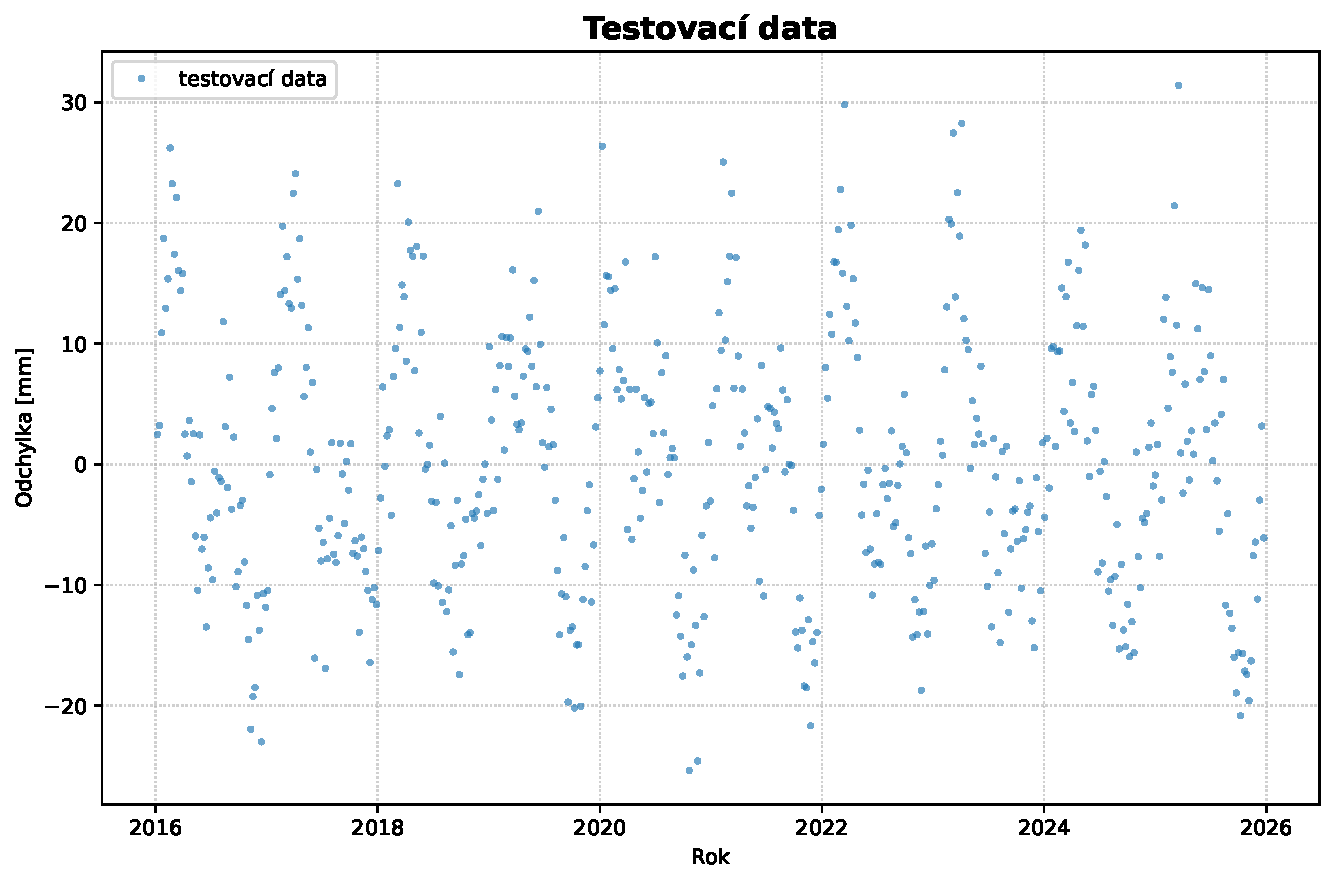
\includegraphics[width=1\linewidth]{images/test/periodicities/test_data.pdf}
  \caption{Syntetická časová řada s~třemi periodickými složkami a šumem}
  \label{fig:test_data}
\end{figure}

\paragraph{FFT periodogram}\leavevmode\\
Pomocí Fourierovy transformace byl vypočten periodogram, ze kterého byly identifikovány dominantní frekvence. Detekované periodicity jsou uvedeny v~tabulce~\ref{tab:fft_significant_peaks}.

\begin{table}[H]
\centering
\small
\caption{Periodické složky detekované metodou FFT.}
\label{tab:fft_significant_peaks}
\begin{tabular}{rrr}
\toprule
Perioda [roky] & Perioda [dny] & Amplituda [mm] \\
\midrule
0.99918 & 364.950 & 10.673 \\
0.55510 & 202.750 & 6.367 \\
0.49959 & 182.475 & 4.679 \\
\bottomrule
\end{tabular}
\end{table}


\noindent Na obrázku~\ref{fig:fft_periodogram} je zobrazen \zk{FFT} periodogram testovacích dat.

\begin{figure}[H]
\centering

\includegraphics[width=1\linewidth]{images/test/periodicities/fft_periodogram.pdf}
\caption{FFT periodogram syntetické časové řady}
\label{fig:fft_periodogram}
\end{figure}


\paragraph{Lomb--Scargleův periodogram}\leavevmode\\
Stejná data byla analyzována pomocí Lomb--Scargleova periodogramu, který je vhodný i pro nepravidelně vzorkované časové řady. Detekované periodicity jsou uvedeny v~tabulce~\ref{tab:lomb_significant_peaks}.

\begin{table}[H]
\centering
\small
\caption{Periodické složky detekované Lomb--Scargleovou metodou.}
\label{tab:lomb_significant_peaks}
\begin{tabular}{rrr}
\toprule
Perioda [roky] & Perioda [dny] & Amplituda [mm] \\
\midrule
1.00156 & 365.819 & 10.693 \\
0.55015 & 200.942 & 6.629 \\
0.49599 & 181.160 & 4.812 \\
1.16689 & 426.208 & 3.439 \\
\bottomrule
\end{tabular}
\end{table}


\noindent Na obrázku~\ref{fig:lomb_periodogram} je znázorněn Lomb--Scargleův periodogram.

\begin{figure}[H]
\centering

\includegraphics[width=1\linewidth]{images/test/periodicities/lomb_scargle_periodogram.pdf}
\caption{Lomb--Scargleův periodogram syntetické časové řady}
\label{fig:lomb_periodogram}
\end{figure}

\paragraph{Zhodnocení výsledků spektrální analýzy}\leavevmode\\
Obě metody úspěšně identifikovaly všechny tři periodické složky přítomné v~testovacích datech. Detekované periody se od skutečných hodnot ve všech případech lišily maximálně v~řádu jednotek dní a~nalezené amplitudy se od skutečných hodnot lišily maximálně v~řádu jednotek milimetrů.

Lomb--Scargleův periodogram má oproti metodě \zk{FFT} výhodu v~tom, že jej lze použít i~pro nepravidelně vzorkované časové řady. V~provedeném testu však detekoval navíc periodicitu o~délce přibližně 426~dní, která v~generovaných datech reálně obsažena nebyla. Metoda \zk{FFT} tuto falešnou periodicitu nedetekovala a~pro pravidelně vzorkovaná data se tak v~provedeném testu jevila jako spolehlivější.

V~dalších analýzách budou proto využívány obě metody vzájemně se doplňujícím způsobem --- \zk{FFT} jako primární nástroj pro pravidelně vzorkované řady a~Lomb--Scargleův periodogram v~případech, kdy jsou v~datech přítomny výpadky nebo nepravidelné vzorkování.

\section{Ověření přesnosti interpolace drah}

Pro porovnání drah družic je nutné převést jednotlivá řešení na společné časové epochy, což lze realizovat například matematickou interpolací. Přesnost interpolace je přitom závislá na zvolené interpolační metodě, charakteru skutečné dráhy družice, hustotě vzorkování a přesnosti vstupních dat. V~ideálním případě nerušeného keplerovského pohybu je dráha družice elipsou a polohu družice by tak bylo možné v~libovolné epoše určit přesně. V~reálných podmínkách je však pohyb družice ovlivněn řadou gravitačních i negravitačních sil, které způsobují odchylky od eliptické dráhy a nelze jej proto dokonale matematicky modelovat.

Pro ověření numerické přesnosti Hermitovy interpolace bylo využito řešení drah družic, které bylo následně uměle zředěno tak, aby vznikly větší časové rozestupy mezi jednotlivými epochami odpovídající různým intervalům vzorkování. V~těchto epochách byly polohy družice určeny interpolací a~porovnány s~původními hustěji vzorkovanými hodnotami, které sloužily jako reference. Pro testování byla využita orbitální řešení \zk{GOP} a~\zk{SSA} pro všechny dostupné družice v~období prvních 30~dní roku 2024, přičemž testování bylo provedeno pro několik různých délek vstupního intervalu. Velikost interpolační chyby byla hodnocena pomocí základních statistických charakteristik vypočtených z~rozdílů poloh (reziduí), konkrétně aritmetického průměru, \zkratka{RMS} a~\zkratka{RMS}0, a~to v~jednotlivých složkách lokálního orbitálního systému \zk{RTN}. Dále byla z~vektoru prostorové vzdálenosti v~každé epoše vyhodnocena celková polohová chyba vyjádřená jako 3D~\zkratka{RMS}. Jako reprezentativní ukázka výsledků je v~následující části uvedeno řešení \zk{GOP} pro družici \zkratka{SARAL}.

\subsubsection{Průběh odchylek interpolace v~rámci jednoho dne}

Na obrázku~\ref{fig:RTN_differences_single_day} jsou znázorněny odchylky polohy v~jednotlivých složkách \zk{RTN} pro první den roku 2024. Graf zachycuje rozdíly mezi původní referenční dráhou se vzorkováním 60~s~a polohami dopočtenými Hermitovou interpolací z~uměle zředěné dráhy se vstupním intervalem 120~s. Odchylky jsou vyjádřeny v~milimetrech.

\begin{figure}[H]
\centering
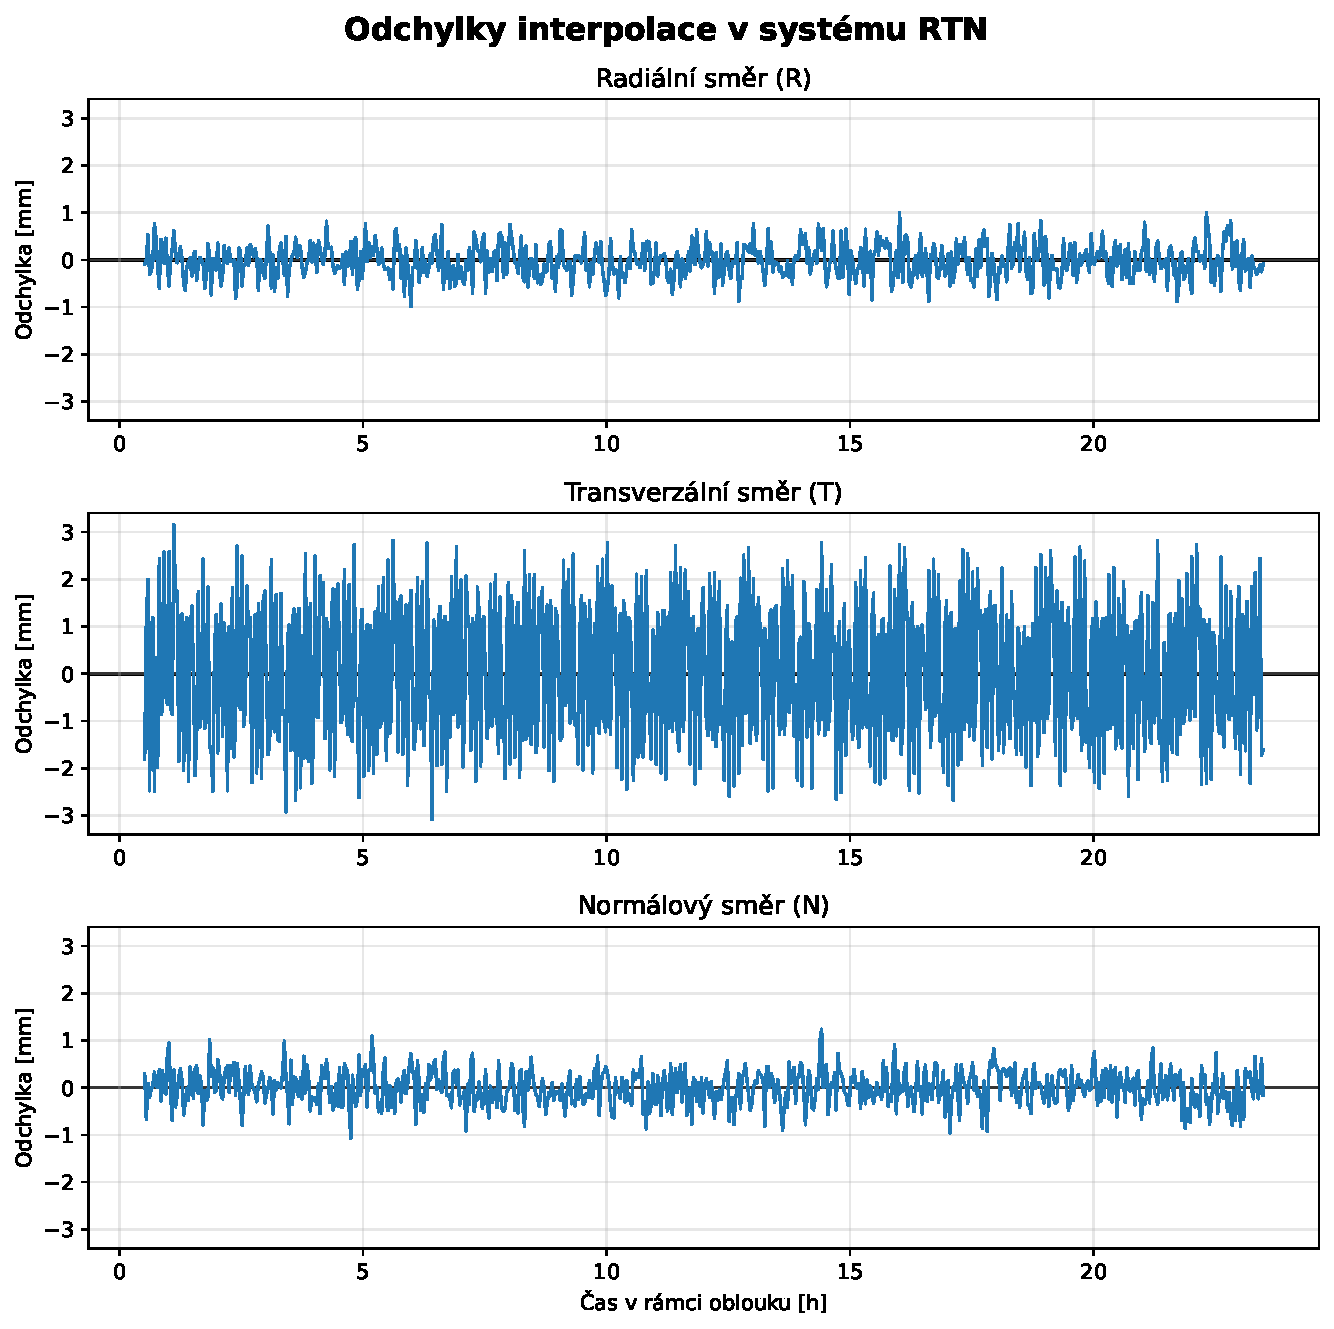
\includegraphics[width=1\linewidth]{images/test/hermite_precision/gop/srl/RTN_differences_single_day.pdf}
\caption{Průběh odchylek interpolace v~systému \zk{RTN} pro 1. 1. 2024}
\label{fig:RTN_differences_single_day}
\end{figure}

Z~obrázku je patrné, že rozdíly interpolované polohy mají hladký průběh bez výrazných skoků. Největší odchylky se vyskytují v~transverzální složce T, která odpovídá směru letu družice a je na interpolační chybu nejcitlivější. Maximální hodnoty odchylek v~radiální a normálové složce se pohybují kolem 1~mm, zatímco v~transverzální složce dosahují až přibližně 3~mm.

Pro podrobnější analýzu charakteru odchylek jsou na obrázku~\ref{fig:RTN_histogram_single_day} uvedeny histogramy jednotlivých složek systému \zk{RTN}. Odchylky jsou vykresleny se zachováním znaménka, což umožňuje posoudit jejich symetrii vzhledem k~nulové hodnotě.

\begin{figure}[H]
\centering
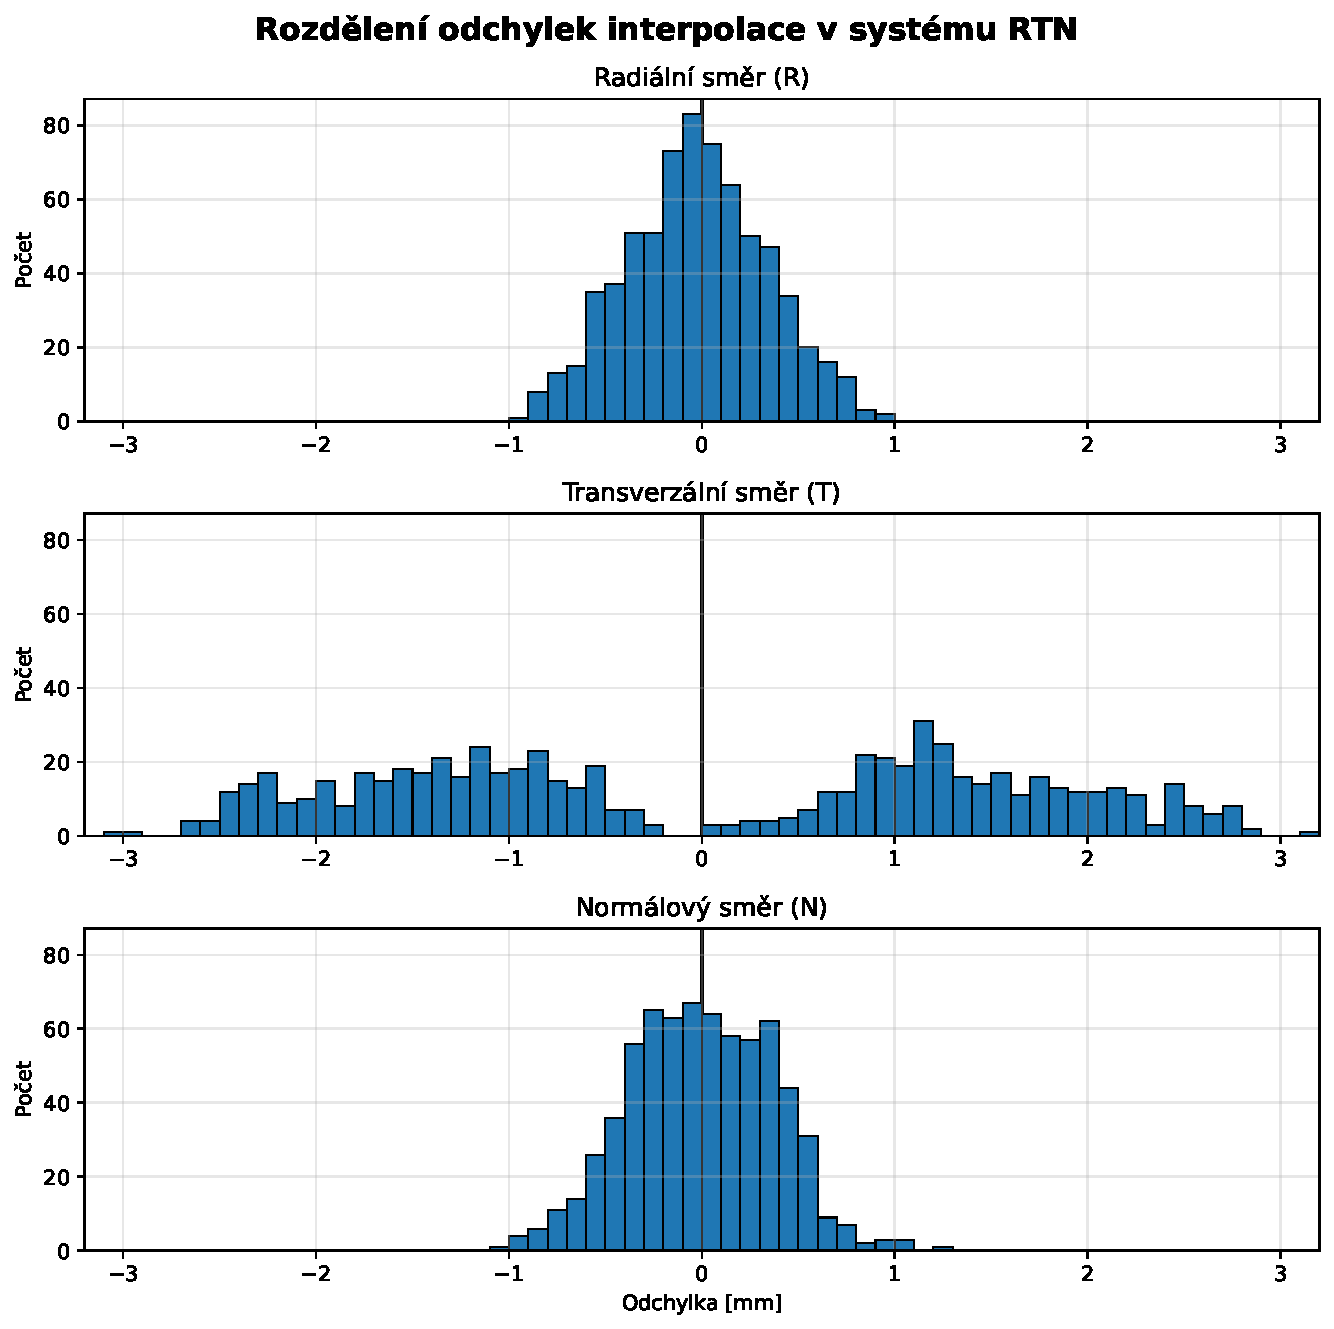
\includegraphics[width=1\linewidth]{images/test/hermite_precision/gop/srl/RTN_histogram_single_day.pdf}
\caption{Histogramy odchylek interpolace v~systému \zk{RTN} pro 1. 1. 2024}
\label{fig:RTN_histogram_single_day}
\end{figure}

Z~histogramů je patrné, že se charakter rozdělení odchylek v~jednotlivých složkách liší. V~radiální a normálové složce jsou odchylky soustředěny v~blízkosti nulové hodnoty a jejich rozsah je výrazně menší než v~transverzálním směru. Naproti tomu v~transverzální složce je rozdělení širší a vykazuje nepravidelný charakter s~častějším výskytem hodnot mimo okolí nulové hodnoty. Vyšší odchylky v~této složce souvisí s~tím, že transverzální směr odpovídá směru letu, který je nejcitlivější na nepřesnosti v~aproximaci trajektorie a vstupních rychlostech Hermitovy interpolace. Odlišný tvar rozdělení v~této složce může naznačovat přítomnost systematické chyby.

Na obrázku~\ref{fig:interp_periodogram} jsou zobrazeny periodogramy odchylek v~jednotlivých složkách systému \zk{RTN}, které slouží k~identifikaci periodických složek v~chybách interpolace.

\begin{figure}[H]
\centering
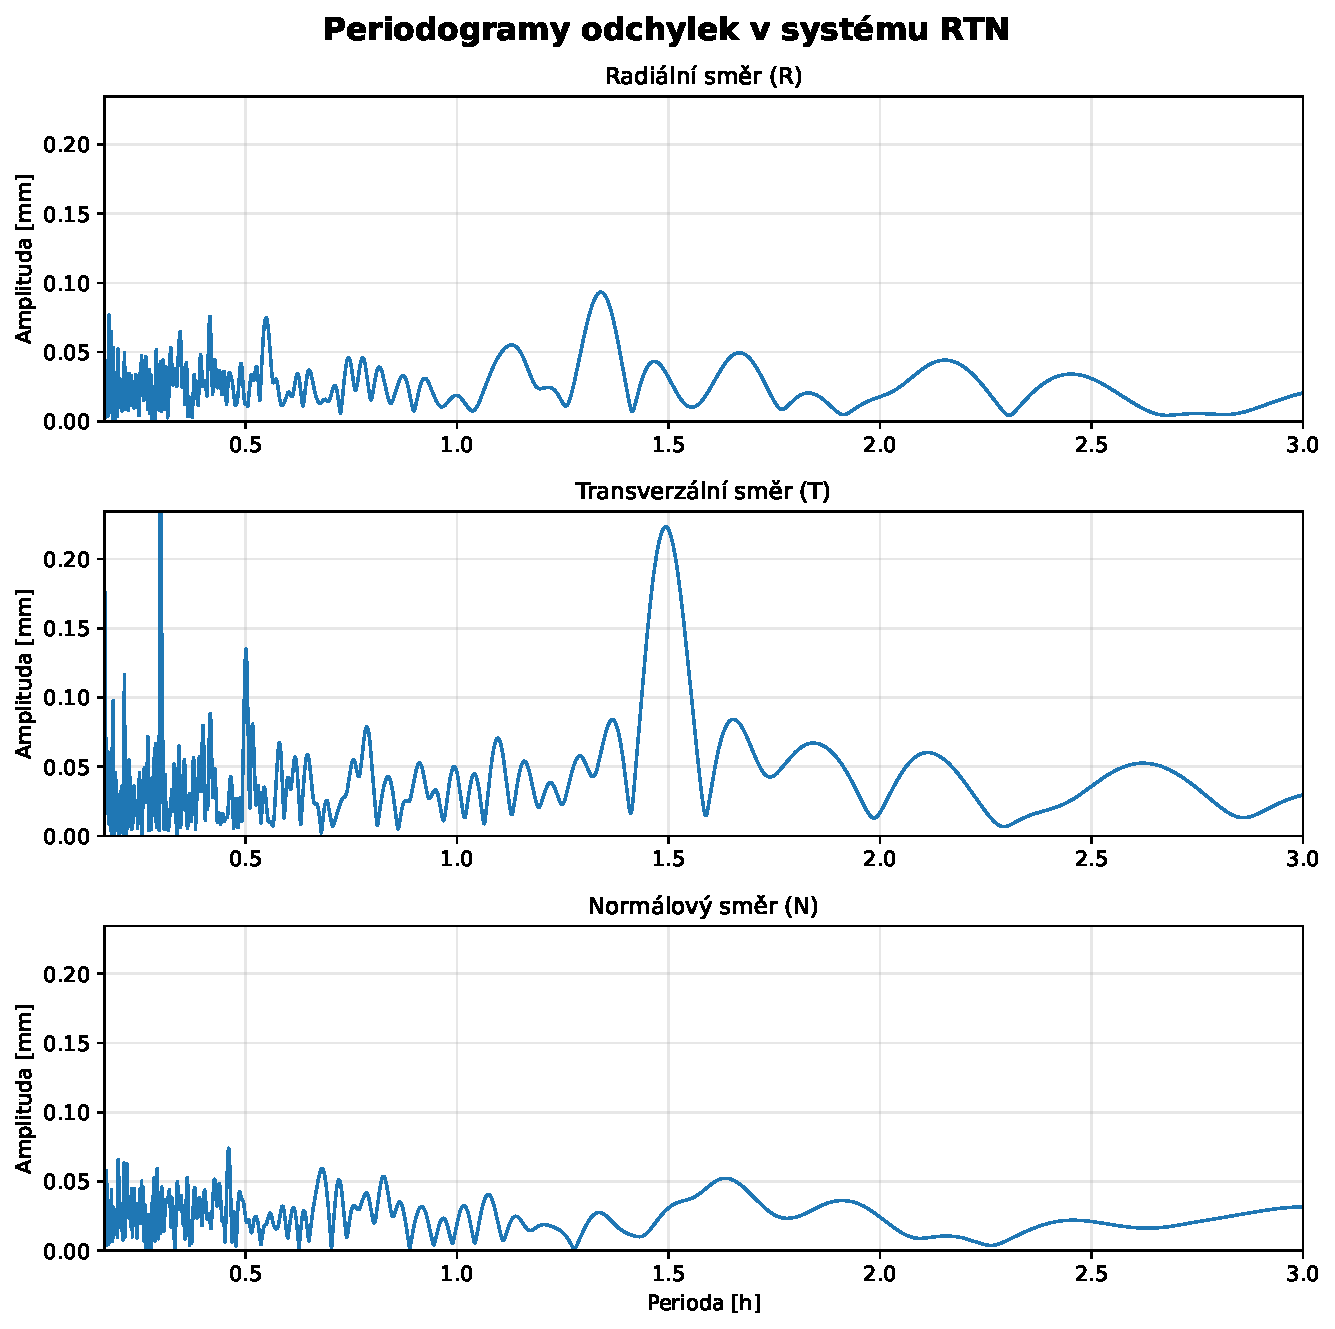
\includegraphics[width=1\linewidth]{images/test/hermite_precision/gop/srl/RTN_lomb_scargle_periodograms_single_day.pdf}
\caption{Periodogramy odchylek interpolace v~systému \zk{RTN} pro 1.~1.~2024}
\label{fig:interp_periodogram}
\end{figure}

Z~periodogramů je patrné, že v~radiální a normálové složce se nevyskytují výrazné dominantní periodicity. Naproti tomu v~transverzální složce je patrná periodická složka s~periodou přibližně 1{,}5~hodiny a amplitudou v~řádu desetin milimetru. Tato perioda přibližně odpovídá oběžné době družice \zkratka{SARAL}, která činí přibližně 100{,}5~minuty. V~grafu je současně patrná také výraznější složka s~periodou kolem 20~minut. Tyto periodicity naznačují, že část interpolační chyby v~transverzálním směru nemá čistě náhodný charakter.

\subsubsection{Stabilita interpolační chyby v~čase}

Pro posouzení stability chyby interpolace ve složkách \zk{RTN} v~delším časovém období byly analyzovány denní hodnoty \zkratka{RMS} pro vstupní interval 120~s. Na obrázku~\ref{fig:Daily_RTN_RMS_over_time} je znázorněn jejich průběh od 1.~1.~2024 do 30.~1.~2024.

\begin{figure}[H]
\centering
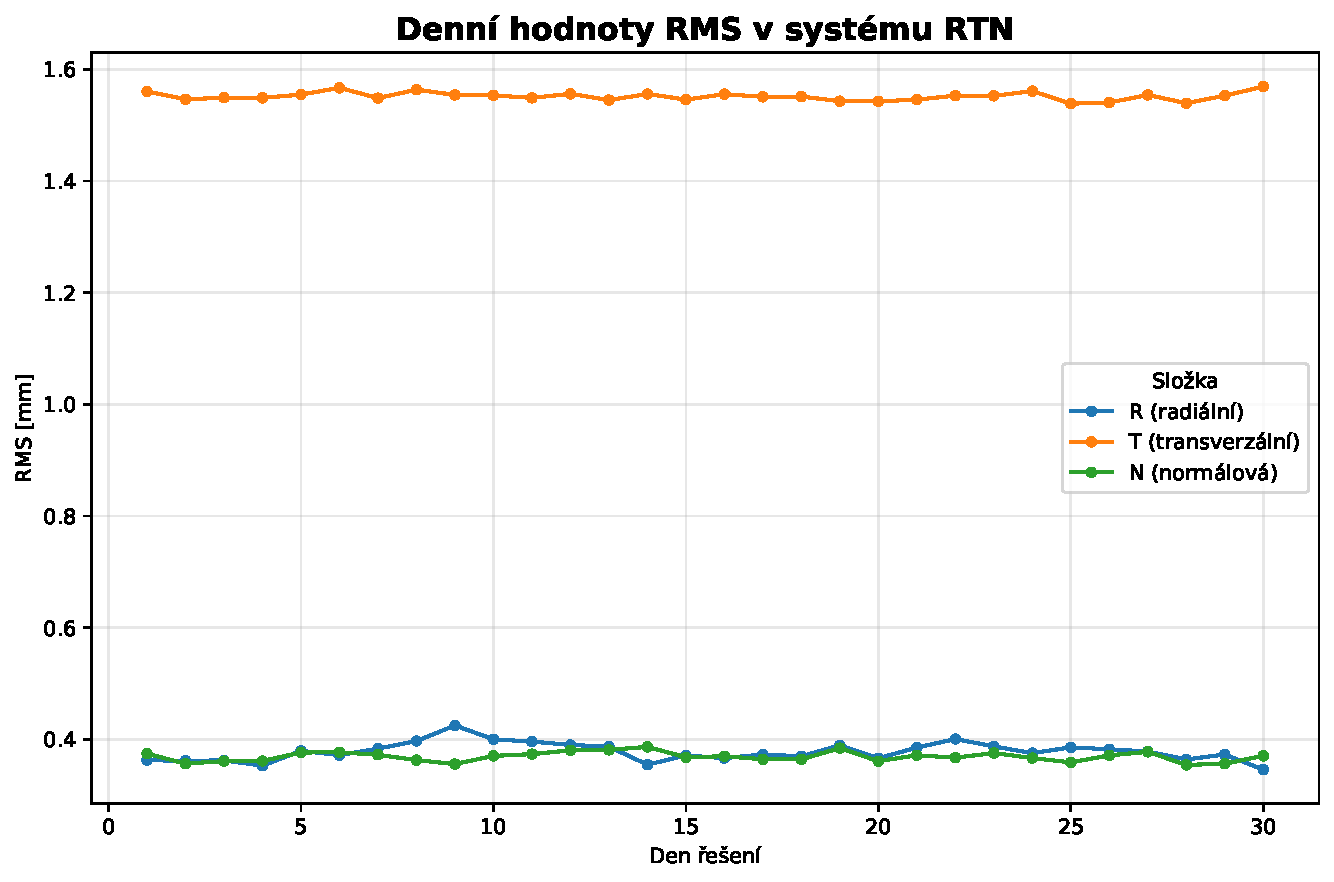
\includegraphics[width=1\linewidth]{images/test/hermite_precision/gop/srl/Daily_RTN_RMS_over_time.pdf}
\caption{Denní hodnoty \zk{RMS} v~systému \zk{RTN} pro vstupní interval 120~s}
\label{fig:Daily_RTN_RMS_over_time}
\end{figure}

Z~grafu je patrné, že hodnoty \zkratka{RMS} v~radiální a normálové složce se stabilně pohybují kolem 0{,}4~mm, zatímco v~nejcitlivější transverzální složce dosahují přibližně 1{,}5~mm. Rezidua jsou v~čase stabilní, bez patrných trendů či skoků. To naznačuje, že použitá Hermitova interpolace 11.~řádu poskytuje v~celém analyzovaném období vnitřně konzistentní výsledky.

\subsubsection{Závislost interpolační chyby na délce vstupního intervalu}

Pro posouzení vlivu vzorkovacího intervalu na přesnost interpolace byla analyzována závislost prostorové chyby na časovém kroku mezi vstupními epochami. Na obrázku~\ref{fig:Daily_3D_RMS_over_time} jsou znázorněny denní hodnoty 3D \zkratka{RMS} pro vybrané intervaly v~průběhu prvních 30~dní roku 2024.

\begin{figure}[H]
\centering
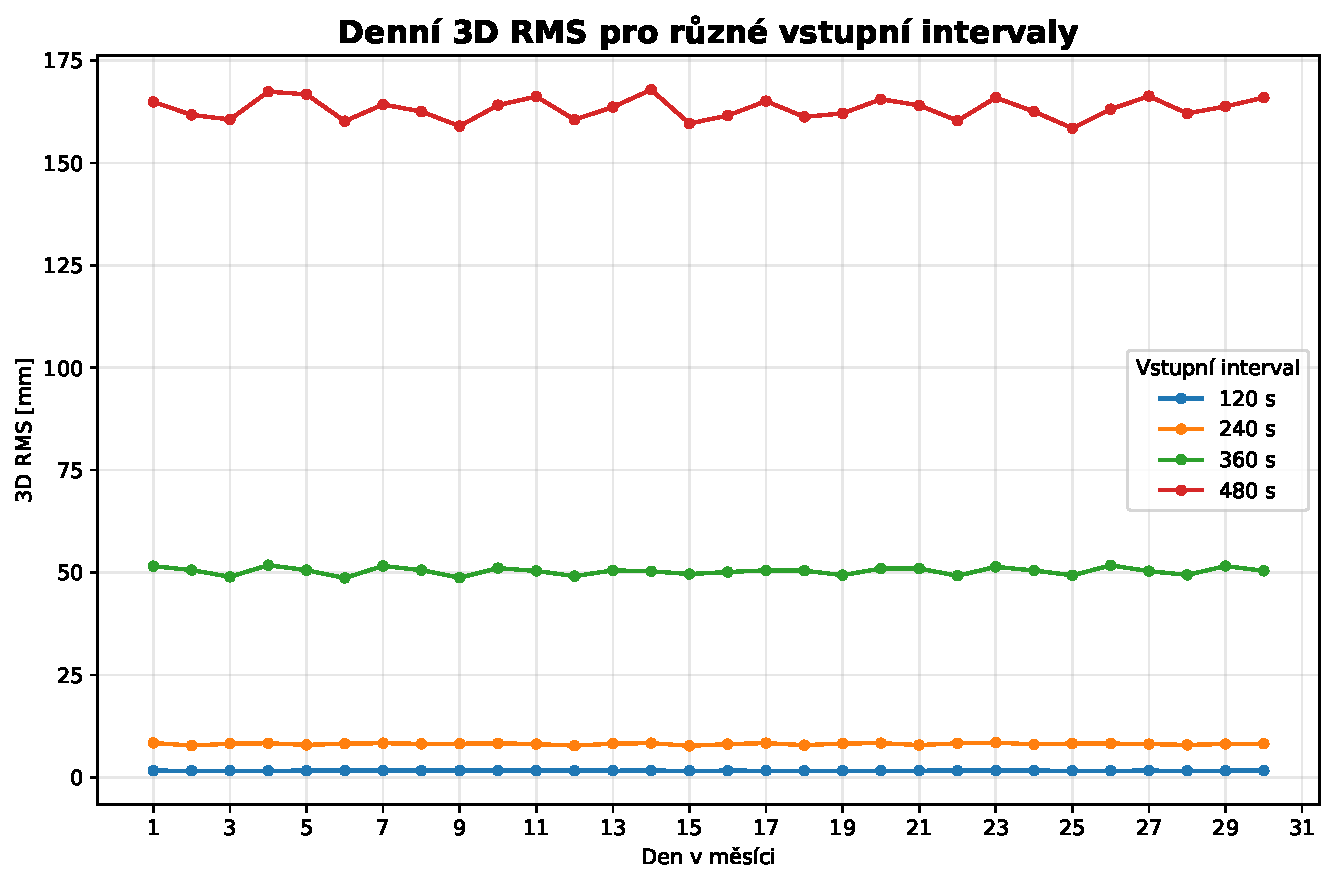
\includegraphics[width=1\linewidth]{images/test/hermite_precision/gop/srl/Daily_3D_RMS_over_time.pdf}
\caption{Denní 3D \zk{RMS} pro různé vstupní intervaly}
\label{fig:Daily_3D_RMS_over_time}
\end{figure}

Z~grafu je patrné, že velikost chyby interpolace výrazně závisí na délce vstupního intervalu. Pro 120~s~dosahuje 3D \zkratka{RMS} nižších jednotek milimetrů, pro 240~s~vyšších jednotek milimetrů a pro 360~s~až 480~s~již desítek až stovek milimetrů. Hodnoty jsou v~čase stabilní, což potvrzuje, že hlavním faktorem přesnosti je délka vstupního intervalu.

Pro kvantitativní shrnutí výsledků jsou v~tabulce~\ref{tab:interp_accuracy} uvedeny souhrnné hodnoty \zk{RMS} interpolační chyby pro jednotlivé vstupní intervaly.

\begin{table}[H]
\centering
\small
\caption{Souhrnné statistiky interpolační chyby pro různé vstupní intervaly}
\label{tab:interp_accuracy}
\begin{tabular}{rrrrr}
\toprule
Interval [s] & R [mm] & T [mm] & N [mm] & 3D RMS [mm] \\
\midrule
120 & 0.378 & 1.552 & 0.369 & 1.639 \\
240 & 5.690 & 5.588 & 1.725 & 8.159 \\
360 & 35.957 & 33.530 & 10.910 & 50.360 \\
480 & 115.936 & 109.275 & 35.632 & 163.254 \\
\bottomrule
\end{tabular}
\end{table}


Z~tabulky je patrné, že s~rostoucím vstupním intervalem dochází k~výraznému nárůstu chyby ve všech složkách systému \zk{RTN}. Pro uměle zředěný interval 120~s~se chyba pohybuje v~řádu milimetrů. V~radiální a normálové složce nepřesahuje 0{,}4~mm a v~transverzální složce dosahuje přibližně 1{,}6~mm. U~delších intervalů chyba narůstá nelineárně a pro krok 480~s~dosahuje celková hodnota 3D \zkratka{RMS} přibližně 163~mm. Tabulka tak potvrzuje, že přesnost interpolace je silně závislá na hustotě vzorkování vstupních epoch.

\subsubsection{Odhad přesnosti pro interval 60~s}

Pro doplnění hodnocení přesnosti byla aproximována závislost celkové chyby 3D \zk{RMS} na délce vstupního intervalu. Výsledná závislost je znázorněna na obrázku~\ref{fig:RMS_3D_vs_interval_estimate}.

\begin{figure}[H]
\centering
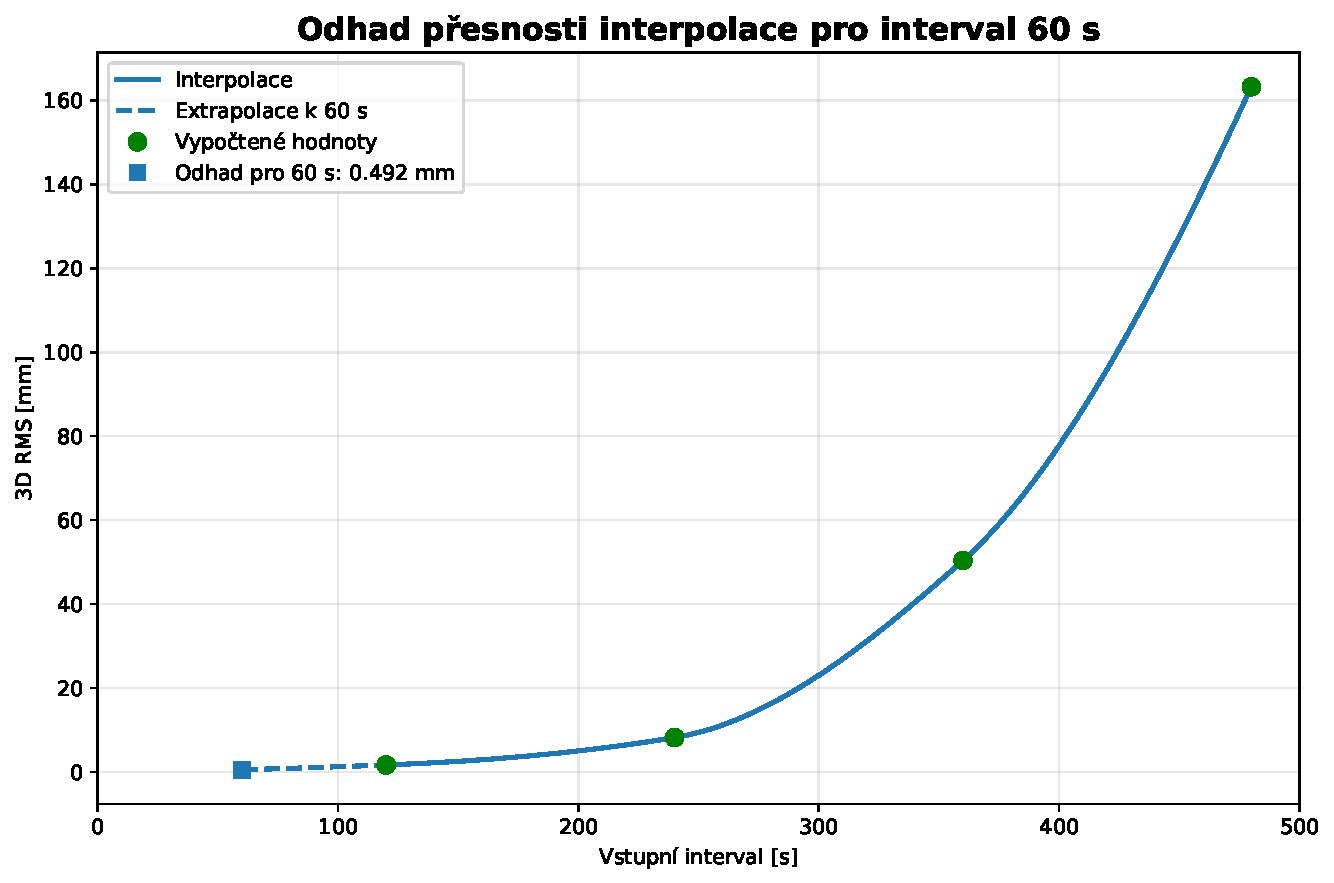
\includegraphics[width=1\linewidth]{images/test/hermite_precision/gop/srl/RMS_3D_vs_interval_estimate_60s.pdf}
\caption{Závislost 3D \zk{RMS} na délce vstupního intervalu}
\label{fig:RMS_3D_vs_interval_estimate}
\end{figure}

Plná část křivky byla interpolována mezi hodnotami vypočtenými pro vstupní intervaly 120--480~s~a znázorňuje nelineární charakter růstu chyby. Přerušovaná část křivky představuje extrapolaci směrem k~intervalu 60~s. Výsledná odhadnutá hodnota 3D \zkratka{RMS} pro interval 60~s~je přibližně 0{,}49~mm. Tato hodnota odpovídá celkovému trendu pozorovanému v~datech a naznačuje, že při vstupním intervalu 60~s~lze očekávat submilimetrovou přesnost interpolace. Uvedený výsledek však nebyl přímo ověřen nezávislou referencí s~hustším vzorkováním, a představuje proto pouze orientační odhad.

\subsubsection{Shrnutí}

Hermitova interpolace poskytuje stabilní výsledky, jejichž přesnost narůstá s~klesajícím intervalem vzorkování. Největší odchylky se vyskytují v~transverzální složce, kde při vzorkování 120~s~nepřesahují jednotky milimetrů (3D \zkratka{RMS} 1{,}6~mm). S~delším intervalem roste chyba nelineárně až na stovky milimetrů. Extrapolace pro krok 60~s~indikuje submilimetrovou přesnost, která by již výrazně neovlivňovala výsledky porovnání drah družic.

\section{Ověření přesnosti parametrizace drah}

Pro ověření přesnosti dynamické parametrizace drah byly bodové dráhy ve formátu \texttt{SP3} parametrizovány v~softwaru Bernese pomocí modulu \texttt{ORBGEN}. Výstupem jsou soubory \texttt{.OUT}, které obsahují statistiky přesnosti parametrizace a~rezidua dynamicky parametrizované dráhy vůči referenčním bodům ze souboru \texttt{SP3} v~lokálním orbitálním systému \zk{RTN}.

Testování bylo provedeno na řešení \zk{SSA} pro družici \zkratka{SARAL} za prvních 30~dní roku 2024. Výpočet byl realizován ve dvou iteracích. Pro testování bylo zvoleno řešení \zk{SSA}, protože řešení \zk{GOP} bylo již určeno pomocí dynamické parametrizace v~softwaru Bernese a~opakovaná parametrizace by tak mohla vést k~nadhodnocení dosažené přesnosti. Přesnost parametrizace byla hodnocena pomocí \zkratka{RMS} reziduí v~jednotlivých složkách systému \zk{RTN} a~celkové prostorové chyby vyjádřené jako 3D~\zkratka{RMS}.

Cílem testování bylo ověřit, zda dynamická parametrizace nezavádí do výsledných drah významné systematické chyby a~zda dosažená přesnost postačuje pro následné porovnání jednotlivých orbitálních řešení.

\subsubsection{Průběh odchylek v~rámci jednoho dne}

Na obrázku~\ref{fig:za_rtn_residuals} je znázorněn průběh epochových reziduí ve složkách
\zk{RTN} pro první den roku 2024.

\begin{figure}[H]
\centering
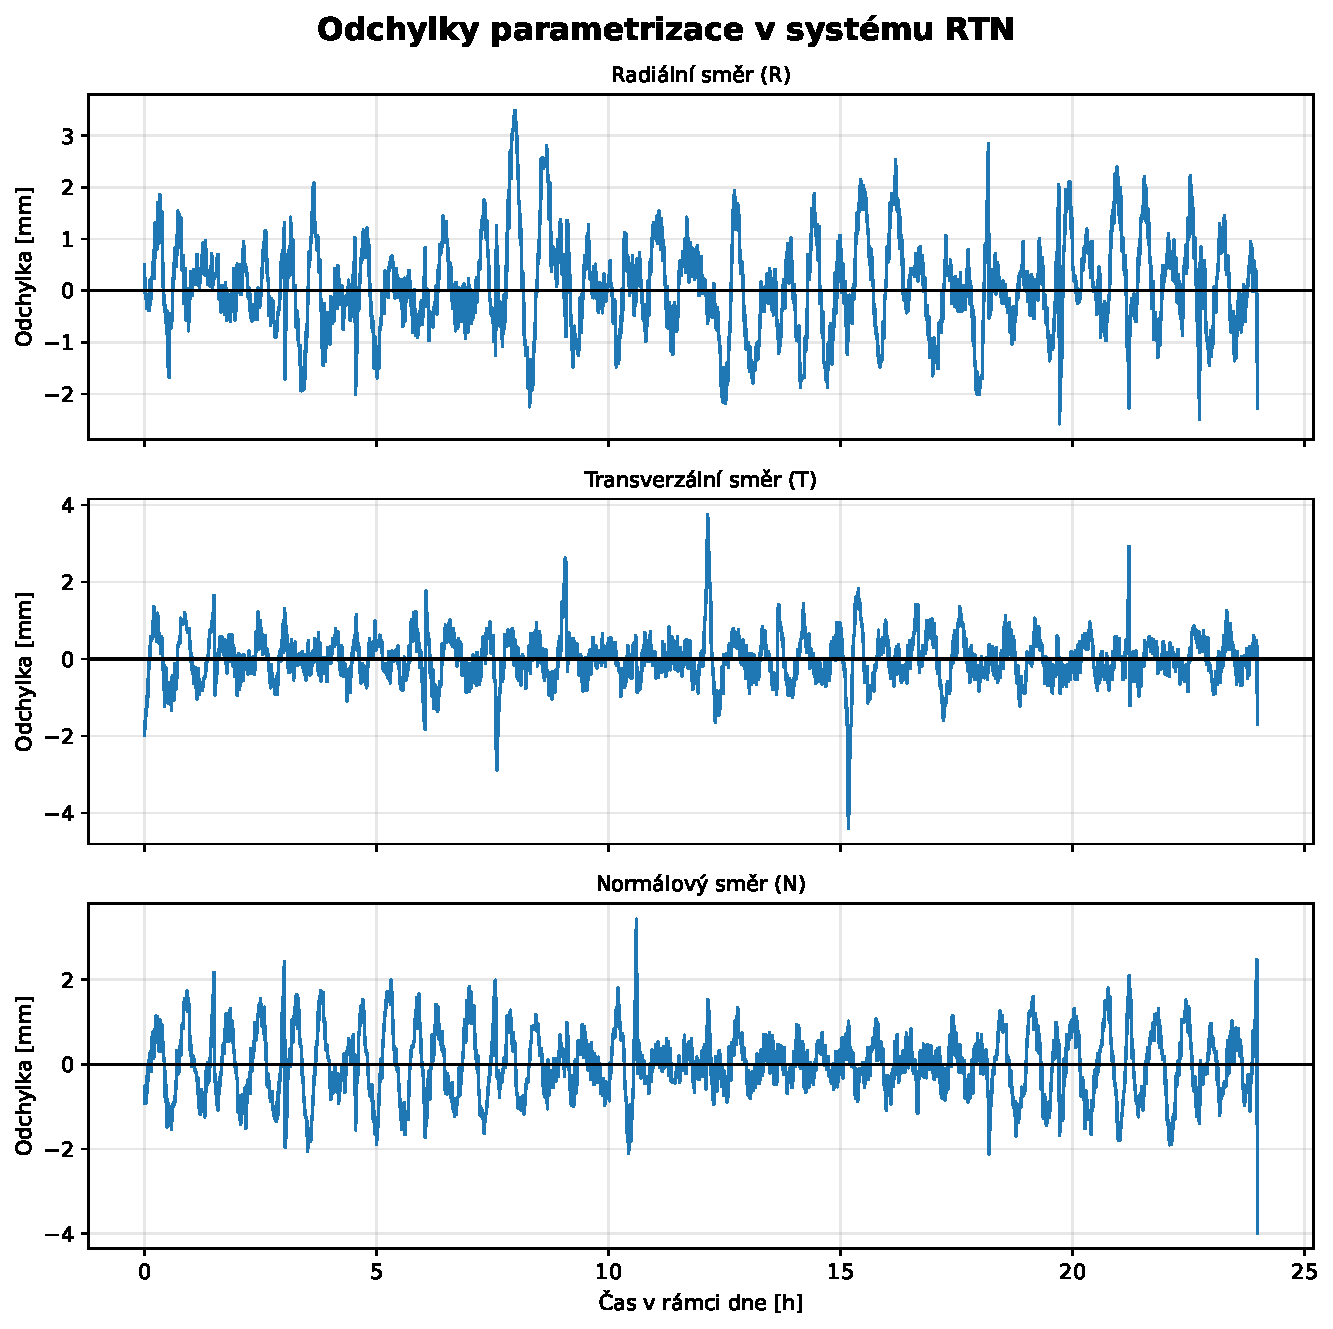
\includegraphics[width=1\linewidth]{images/test/dynamic_precision/sa_za_rtn_residuals_doy001_iter2.pdf}
\caption{Průběh odchylek parametrizace v~systému \zk{RTN} pro 1.~1.~2024}
\label{fig:za_rtn_residuals}
\end{figure}

Z~grafu je patrné, že odchylky mají plynulý průběh bez výrazných skoků, přičemž jejich
charakter se mění v~závislosti na konkrétním dynamickém oblouku. Odchylky v~radiální
složce dosahují hodnot až přibližně 3,5~mm, v~transverzální složce pak až 4,4~mm
a v~normálové složce do~4~mm.

Pro posouzení statistického rozložení odchylek jsou na obrázku~\ref{fig:za_rtn_histograms}
znázorněny histogramy reziduí v~jednotlivých složkách \zk{RTN}.

\begin{figure}[H]
\centering
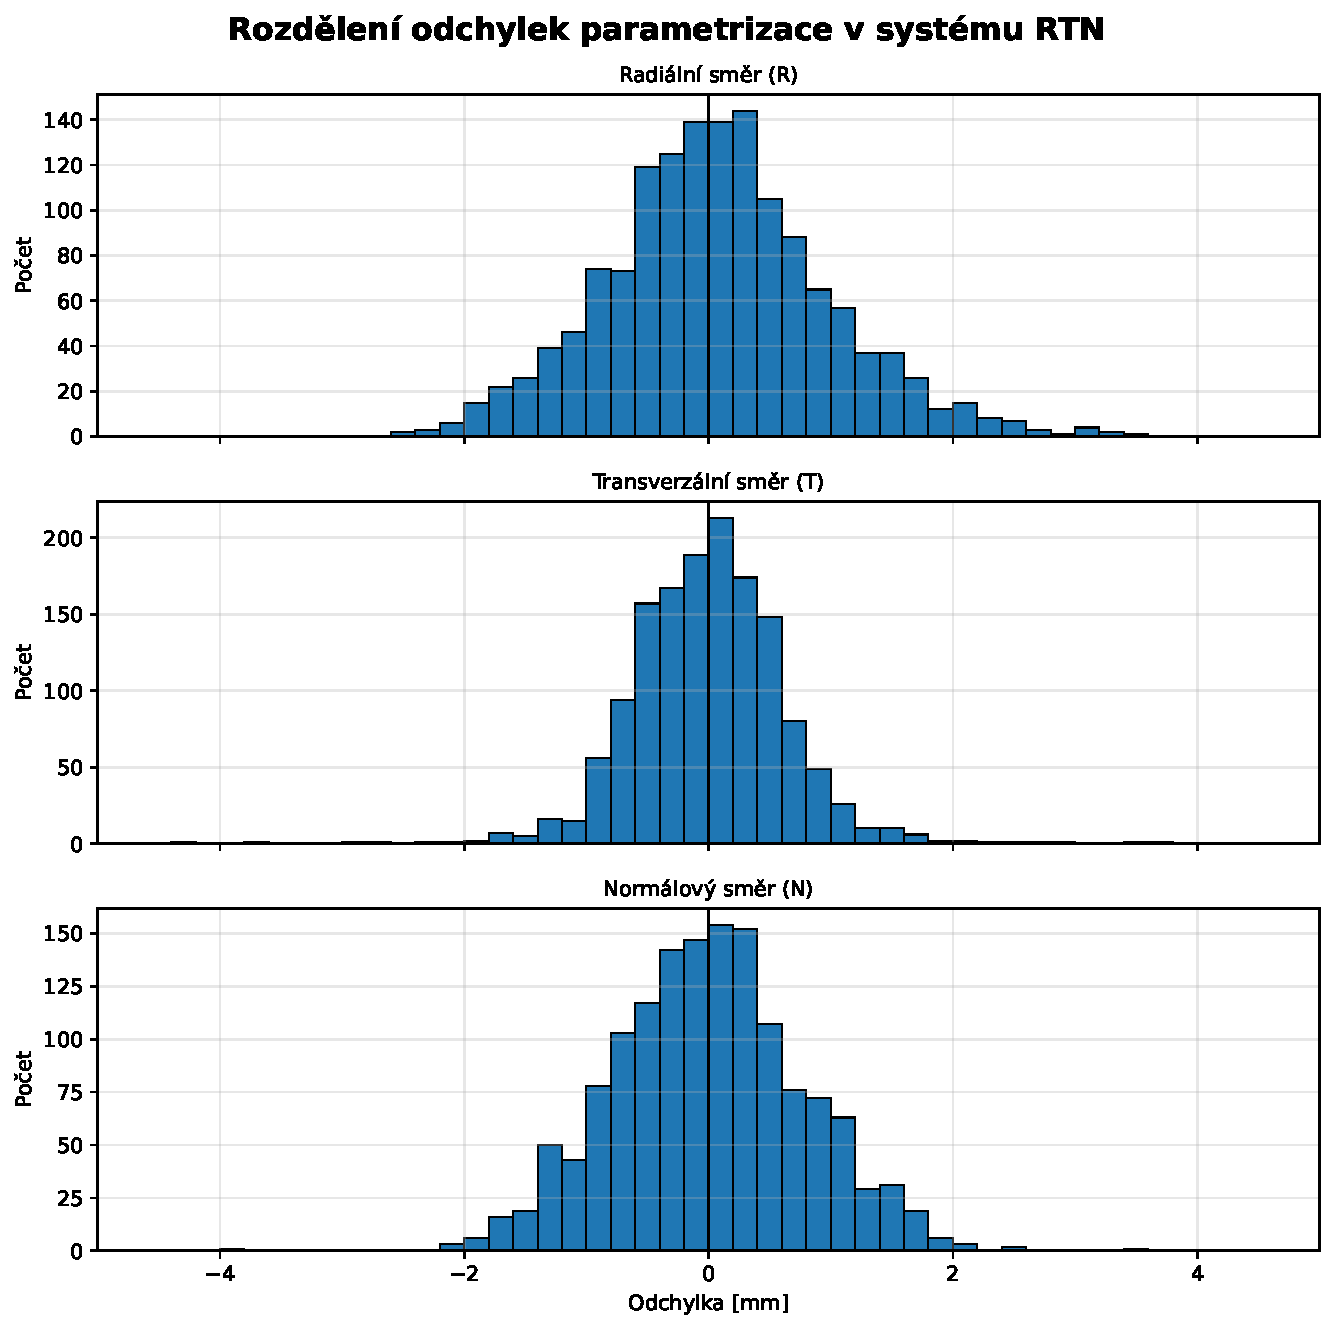
\includegraphics[width=1\linewidth]{images/test/dynamic_precision/sa_za_rtn_histograms_doy001_iter2.pdf}
\caption{Histogramy odchylek parametrizace v~systému \zk{RTN} pro 1.~1.~2024}
\label{fig:za_rtn_histograms}
\end{figure}

Z~histogramů je patrné, že odchylky jsou ve všech třech složkách soustředěny v~blízkosti
nulové hodnoty a vykazují přibližně symetrické rozdělení. Tento charakter naznačuje
absenci výrazných systematických odchylek.

\subsubsection{Spektrální analýza odchylek}

Pro identifikaci případných periodických složek v~odchylkách parametrizace byl vypočten
Lombův--Scargleův periodogram epochových reziduí. Na obrázku~\ref{fig:za_rtn_periodograms}
jsou znázorněny periodogramy pro složky \zk{RTN}.

\begin{figure}[H]
\centering
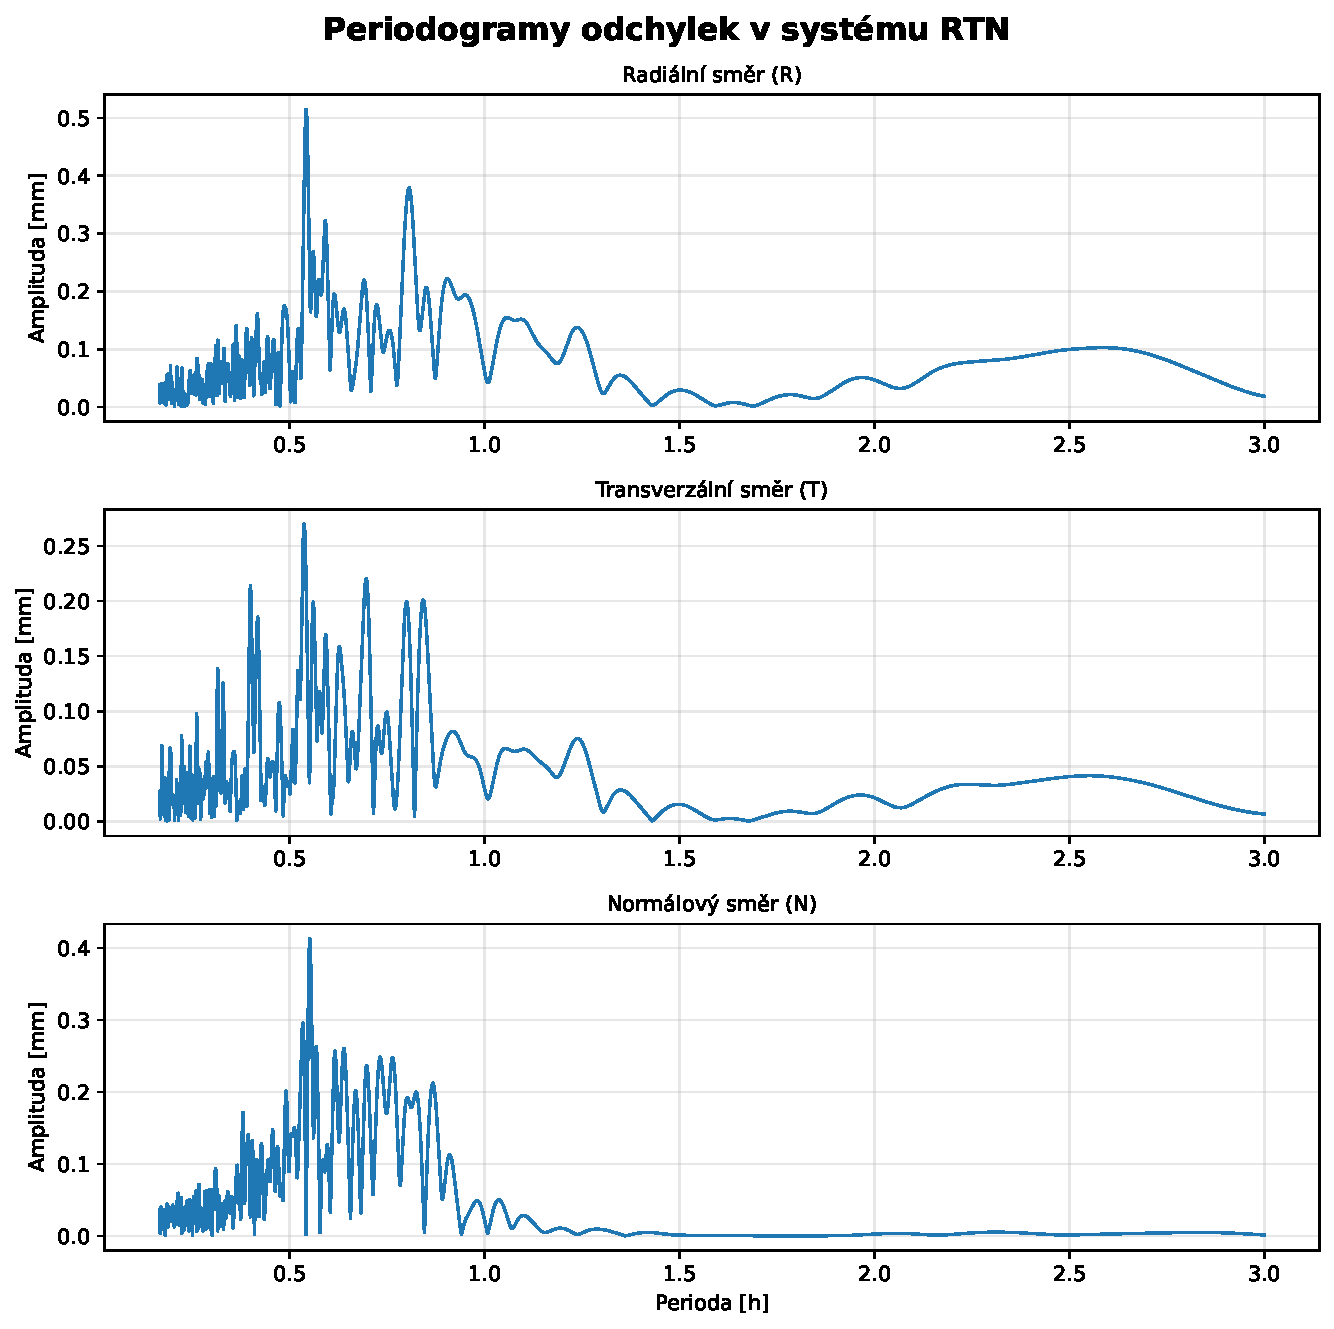
\includegraphics[width=1\linewidth]{images/test/dynamic_precision/sa_za_rtn_periodograms_doy001_iter2.pdf}
\caption{Periodogramy odchylek parametrizace v~systému \zk{RTN} pro 1.~1.~2024}
\label{fig:za_rtn_periodograms}
\end{figure}

Periodogramy naznačují přítomnost několika slabších periodických složek s~periodami přibližně kolem 0{,}5~h a amplitudami řádově v~desetinách milimetru. Tyto složky pravděpodobně nesouvisí přímo s~oběžnou dobou družice \zkratka{SARAL}, která je výrazně delší, ani s~délkou použitého parametrizačního oblouku. Jejich zjevnou příčinu se nepodařilo určit. Vzhledem k~nízkým amplitudám je lze považovat spíše za šum nebo drobný numerický projev parametrizace než za významný zdroj chyb.

\subsubsection{Stabilita přesnosti v~čase}

Pro posouzení časové stability přesnosti jsou na obrázku~\ref{fig:za_daily_rms} znázorněny denní hodnoty \zkratka{RMS} v~průběhu prvních 30~dní roku 2024.

\begin{figure}[H]
\centering
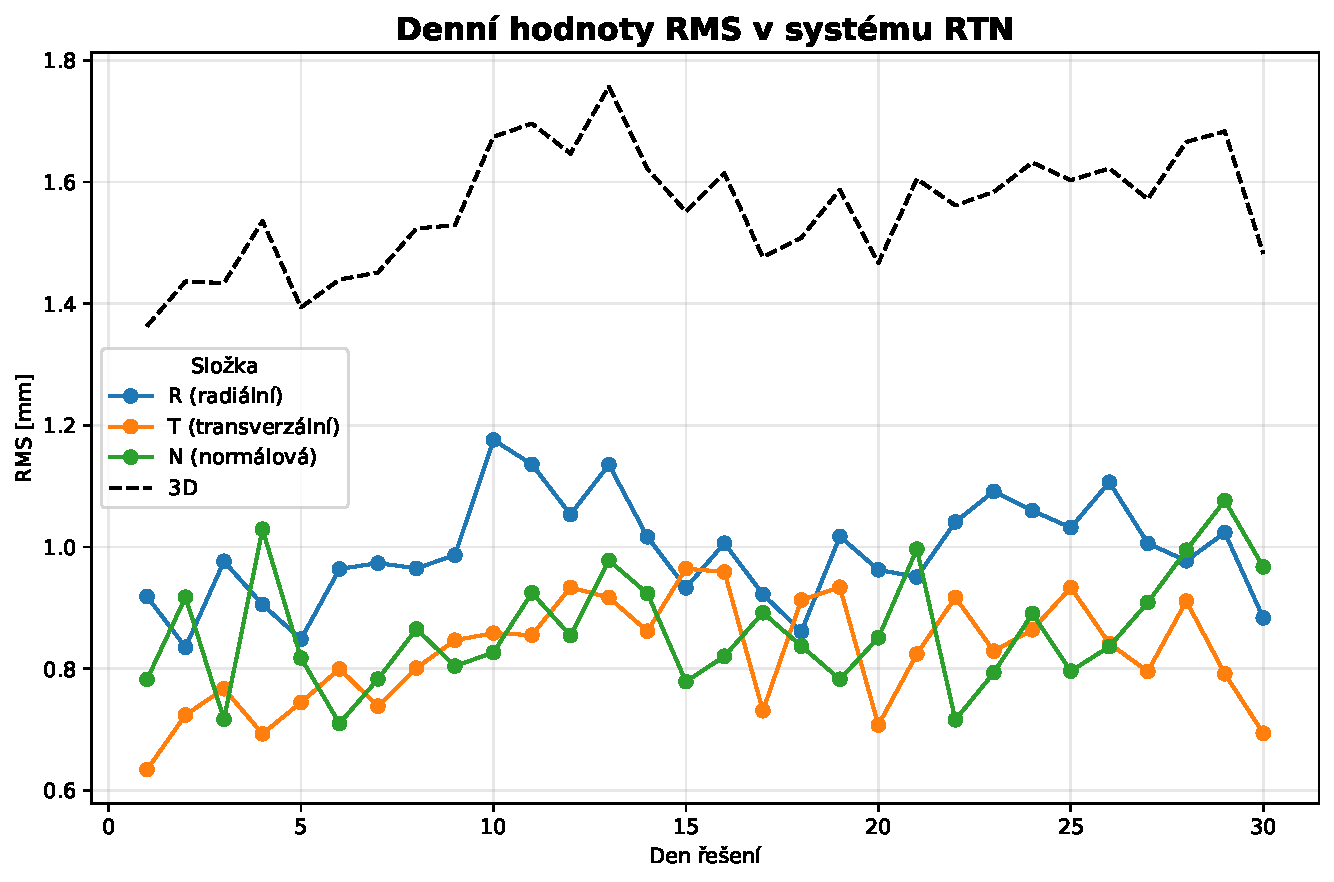
\includegraphics[width=1\linewidth]{images/test/dynamic_precision/sa_za_daily_rms_doy001_030_iter2.pdf}
\caption{Denní hodnoty \zk{RMS} parametrizace v~systému \zk{RTN}}
\label{fig:za_daily_rms}
\end{figure}

Denní hodnoty \zk{RMS} nevykazují výrazné trendy ani skoky, což naznačuje časově stabilní přesnost parametrizace. Souhrnné statistiky vypočtené z~jednotlivých epoch za celé analyzované období (prvních 30~dní roku 2024) jsou uvedeny v~tabulce~\ref{tab:sa_za_rms_summary}.

\begin{table}[H]
\centering
\small
\caption{Souhrnné statistiky parametrizace pro prvních 30~dní roku 2024}
\label{tab:sa_za_rms_summary}
\begin{tabular}{lrrr}
\toprule
Složka & Průměr [mm] & RMS [mm] & Max. abs. reziduum [mm] \\
\midrule
R & 0.104 & 0.996 & 5.460 \\
T & -0.000 & 0.831 & 9.490 \\
N & 0.007 & 0.867 & 23.130 \\
3D & 1.372 & 1.560 & 23.641 \\
\bottomrule
\end{tabular}
\end{table}


\subsubsection{Shrnutí}

Dynamická parametrizace dráhy v~softwaru Bernese vykazuje v~celém analyzovaném období stabilní přesnost. Hodnoty \zk{RMS} epochových reziduí se ve všech složkách systému \zk{RTN} pohybují v~řádu nižších jednotek milimetrů. Spektrální analýza současně neodhalila výrazné periodické složky, což naznačuje absenci významných systematických periodických chyb parametrizace.
\chapter{Výsledky}
\label{7-vysledky}

Výsledky této práce jsou rozděleny do dvou částí podle analyzovaných dat -- na~analýzu časových řad souřadnic stanic systému \zkratka{DORIS} a~na~analýzu přesných drah družic vybavených přijímačem signálu systému \zkratka{DORIS}. Vzhledem k~objemu výsledků je v~hlavním textu uveden kompletní postup analýzy vždy na~jednom ukázkovém případu, který ilustruje celý analytický řetězec od~vstupních dat po~interpretaci. Pro~ostatní analyzované stanice a~družice jsou uvedeny pouze přehledy nalezených výsledků. Kompletní analýzy jsou obsaženy v~samostatných reportech tvořících přílohy této práce. Všechny grafy byly vytvořeny pomocí knihovny \texttt{matplotlib} v~jazyce Python.

\section{Časové řady}
\label{sec:casove-rady}

Analyzovány byly časové řady souřadnic stanic systému \zkratka{DORIS} za~období 2015 až 2025 s~využitím produktu STCD z~kumulativního řešení analytického centra GOP (verze gop25wd04), vzorkovaného s~týdenním krokem. Pro~analýzu byly vybrány stanice, jejichž chování bylo v~interním přehledu \zkratka{IDS} označeno jako podezřelé. U~stanic, kde v~analyzovaném období došlo k~výměně vysílače, je uveden identifikátor použitý pro analyzovanou časovou řadu:

\begin{itemize}
\item \textbf{KIVC} -- Kitab, Uzbekistán
\item \textbf{JIWC} -- Jiufeng, Čína
\item \textbf{LICB} -- Libreville, Gabon
\item \textbf{SARC} -- Sal, Kapverdy
\item \textbf{STKC} -- St.~John's, Kanada
\item \textbf{CADB} -- Cachoeira, Brazílie
\item \textbf{THUB} -- Thule, Grónsko
\item \textbf{MSPB} -- Mount Stromlo, Austrálie
\item \textbf{KRWB} -- Kourou, Francouzská Guyana
\end{itemize}

Cílem analýzy bylo indikované podezřelé chování potvrdit nebo vyvrátit, popsat jeho charakter a~pokusit se nalézt pravděpodobnou příčinu. Pro~každou stanici byl nejprve odhadnut lineární trend a~následně model s~jedním či více zlomy, který umožňuje zachytit skoky i~změny sklonu. Vhodnost jednotlivých modelů byla porovnána pomocí \zkratka{BIC}. Na~detrendovaných datech byla provedena spektrální analýza a~detekce diskontinuit dvěma nezávislými metodami. Výsledky byly ověřeny porovnáním s~blízkými stanicemi na~téže litosférické desce a~s~nezávislými kombinačními řešeními jiných analytických center.

V~následující části je podrobně popsán postup analýzy na~ukázkové stanici KIVC~-- Kitab, Uzbekistán. Tato stanice byla zvolena, protože je v~její časové řadě patrná změna trendu, skok i~periodická složka. Souhrnné výsledky pro~všechny analyzované stanice jsou uvedeny v~kapitole~\ref{sec:souhrn-casove-rady}, detailní analýzy jednotlivých stanic jsou obsaženy v~příloze.

\subsection{Ukázka analýzy: stanice KIVC~-- Kitab, Uzbekistán}

\subsubsection{Surová data}

Na obrázku~\ref{fig:kivc_raw} jsou znázorněny surové časové řady souřadnic stanice KIVC ve složkách dE, dN a dU za analyzované období.

\begin{figure}[H]
    \centering
    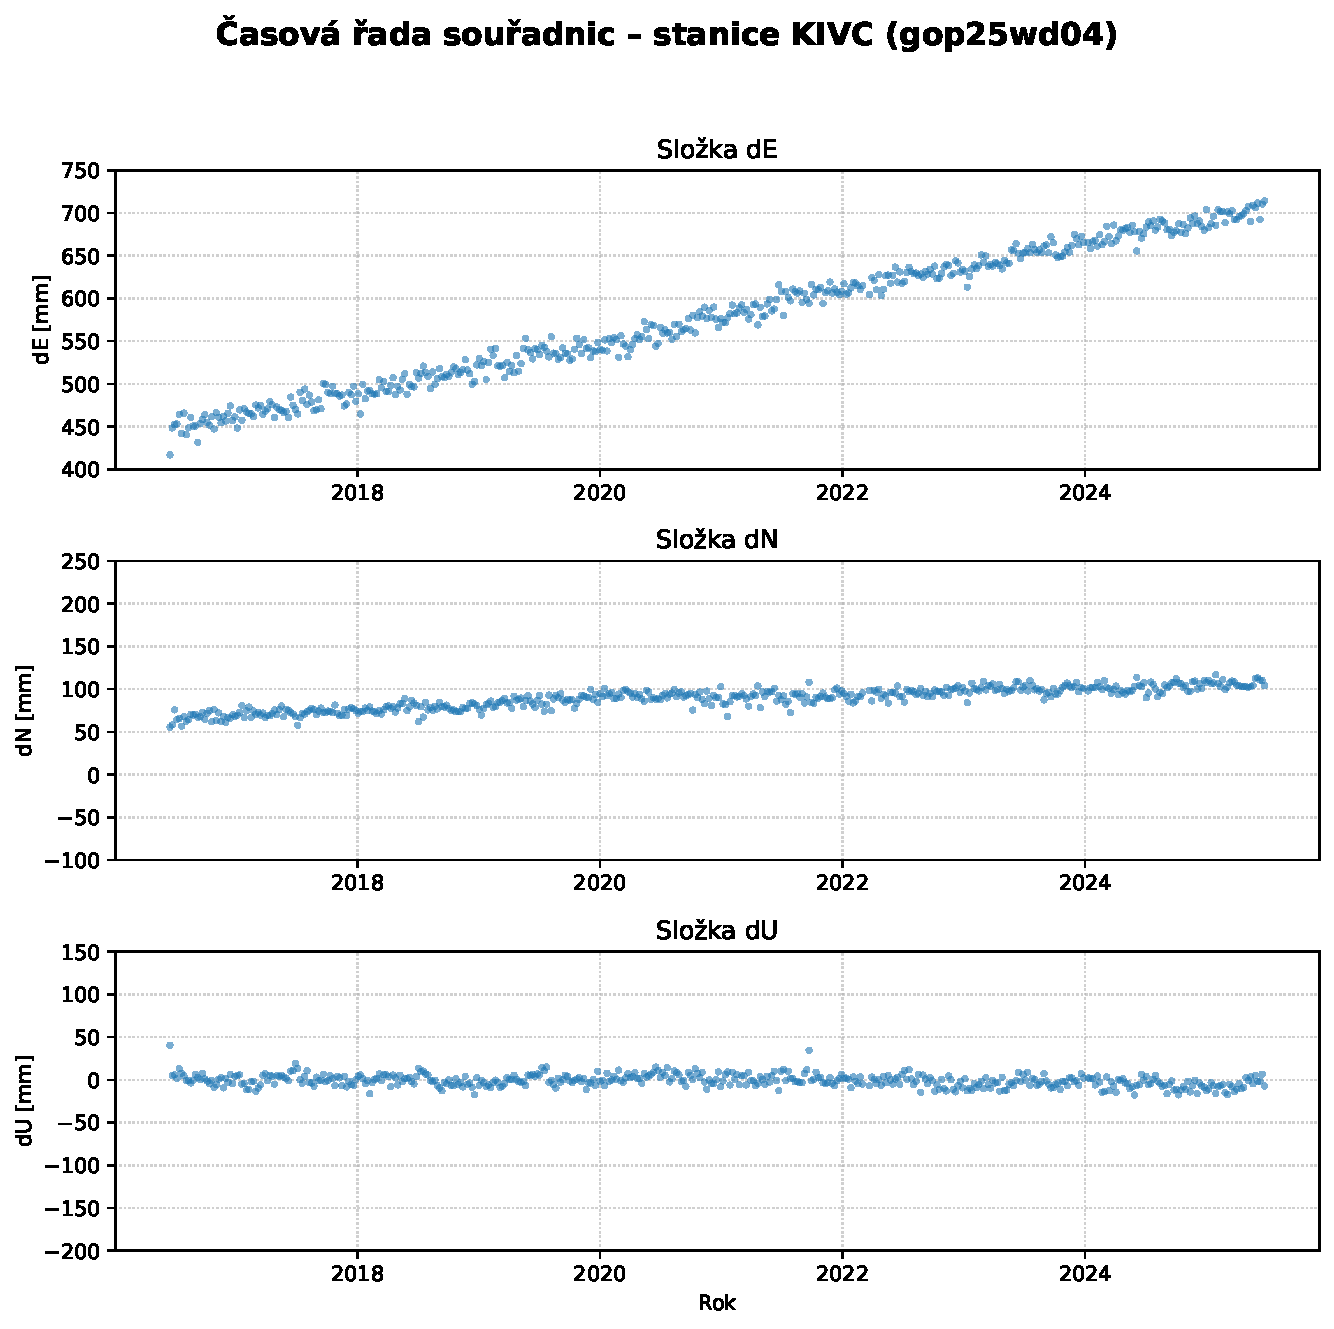
\includegraphics[width=1\textwidth]{images/results/stations/kivc/gop25wd04_stcd_kivc_raw_data.pdf}
    \caption{Surová časová řada souřadnic stanice KIVC (dE, dN, dU)}
    \label{fig:kivc_raw}
\end{figure}

\subsubsection{Lineární trend}

Na obrázku~\ref{fig:kivc_trend_1seg} je znázorněn vážený lineární trend časové řady souřadnic stanice KIVC, při jehož odhadu byly použity váhy \(p_i = 1/\sigma_i^2\). Z~výsledků je patrný výrazný lineární trend především ve složce dE, kde byla odhadnuta směrnice přibližně 29{,}1~mm/rok. Ve složce dN dosahuje trend přibližně 4{,}2~mm/rok a ve vertikální složce dU je trend mírně záporný, přibližně $-0{,}7$~mm/rok.

\begin{figure}[H]
    \centering
    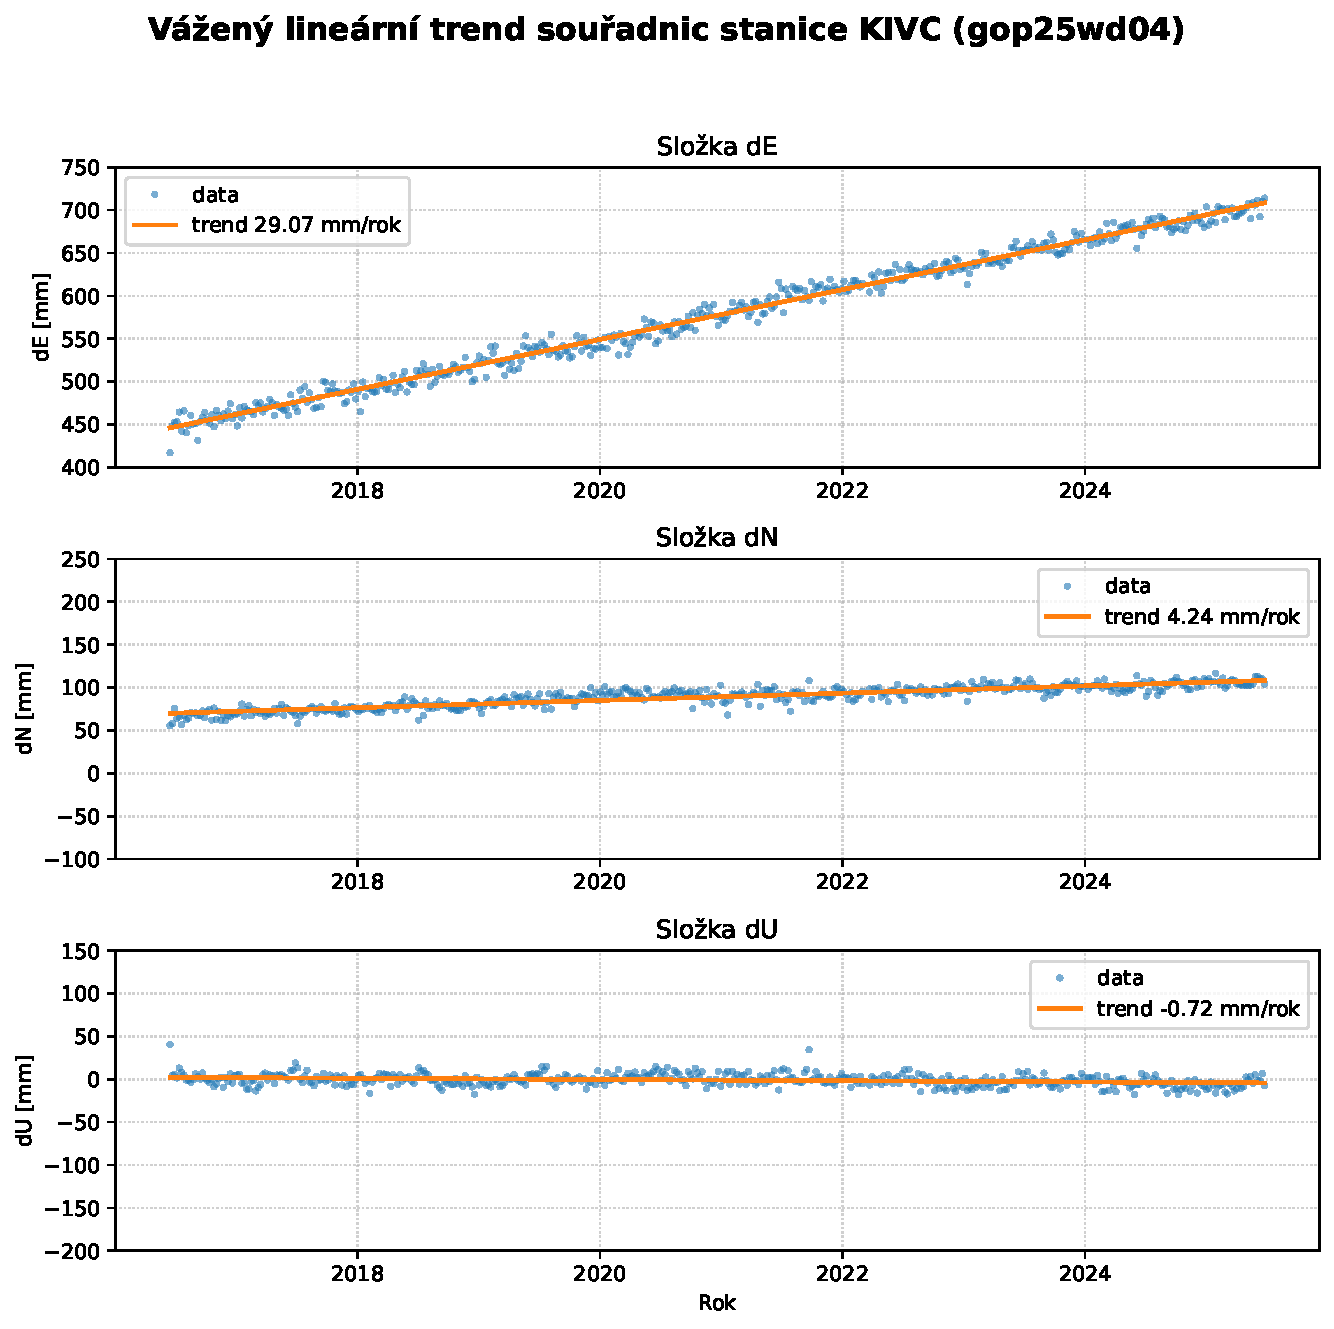
\includegraphics[width=1\textwidth]{images/results/stations/kivc/gop25wd04_stcd_kivc_trend_weighted_1seg.pdf}
    \caption{Vážený lineární trend souřadnic stanice KIVC}
    \label{fig:kivc_trend_1seg}
\end{figure}

Rezidua po odečtení lineárního trendu (obr.~\ref{fig:kivc_res_1seg}) naznačují přítomnost nenáhodných složek, což může znamenat, že lineární model není pro popis časové řady dostatečný.

\begin{figure}[H]
    \centering
    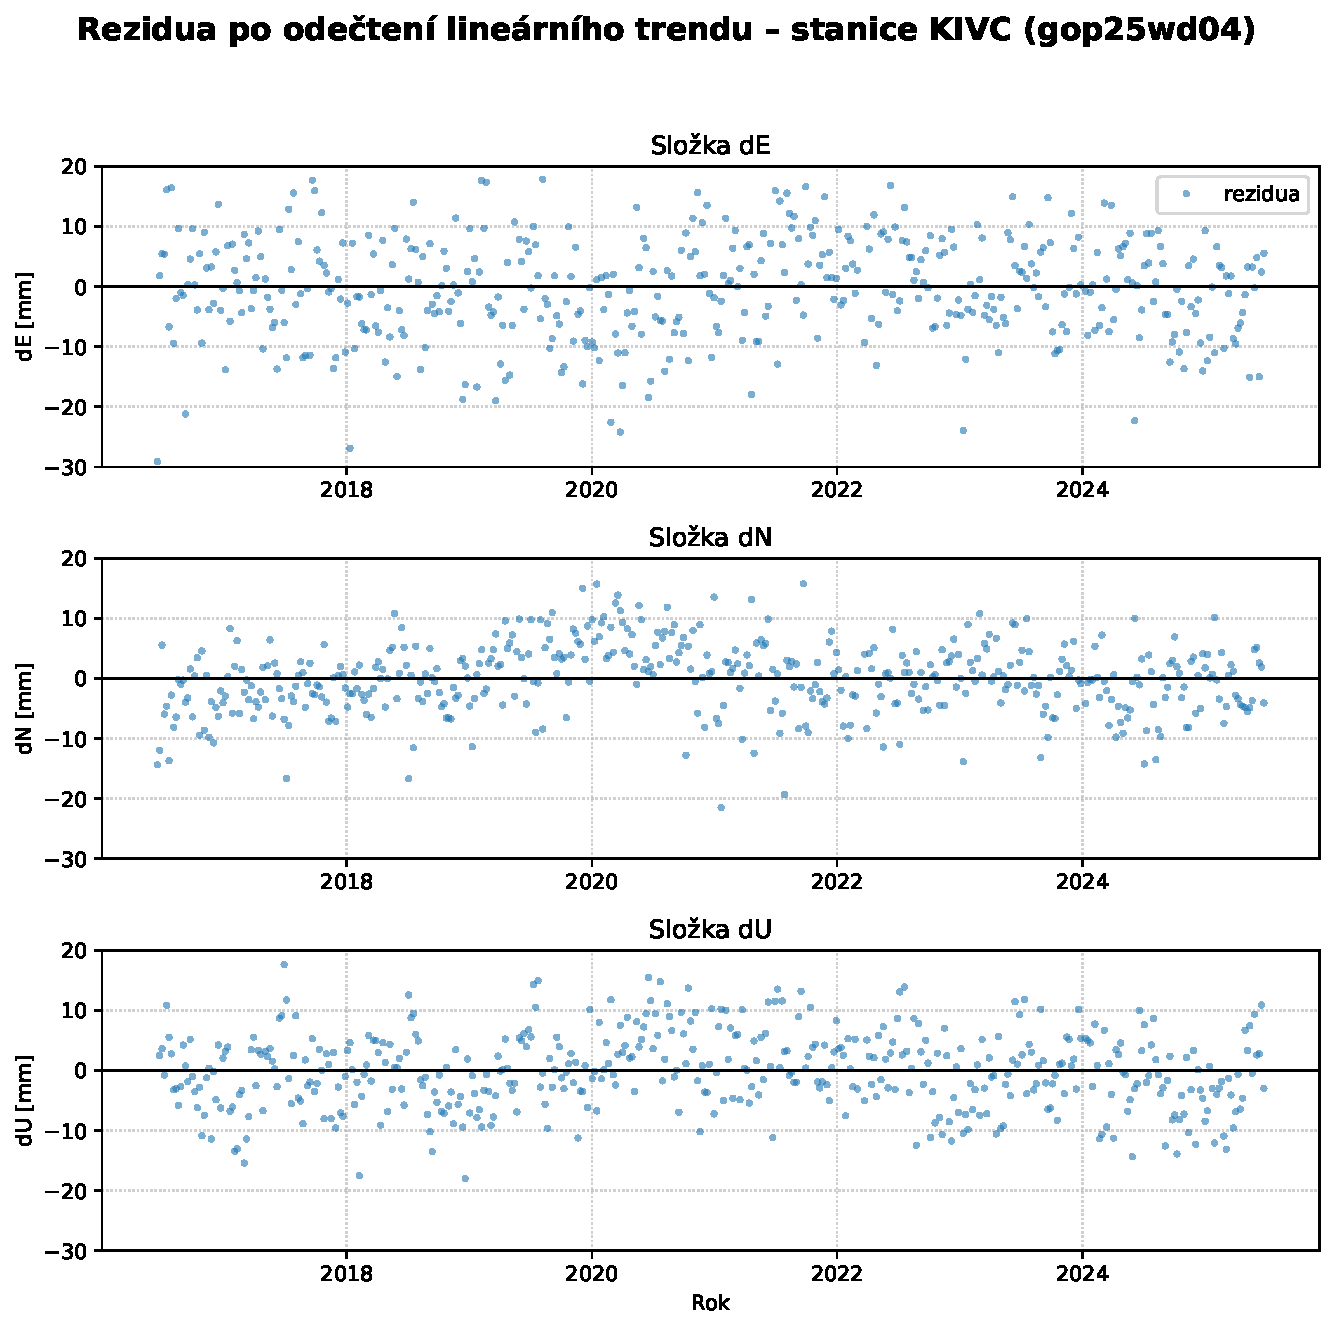
\includegraphics[width=1\textwidth]{images/results/stations/kivc/gop25wd04_stcd_kivc_residuals_weighted_1seg.pdf}
    \caption{Rezidua po odečtení lineárního trendu stanice KIVC}
    \label{fig:kivc_res_1seg}
\end{figure}

\subsubsection{Model se zlomy}

Pro zpřesnění popisu časové řady byl použit model se zlomy umožňující zachytit skoky a~změny trendu v~jednotlivých složkách souřadnic. Model byl odhadnut samostatně pro složky dE, dN a~dU, přičemž poloha
bodů zlomu byla určena iterativně na základě minimalizace hodnoty \zk{BIC}.

Na obrázku~\ref{fig:kivc_trend_breaks} je znázorněn výsledný model se zlomy a~v~tabulce~\ref{tab:gop25wd04_stcd_kivc_trend_weighted_multiseg} jsou shrnuty identifikované body zlomu včetně odhadnutých velikostí skoků a~změn trendu.

\begin{figure}[H]
    \centering
    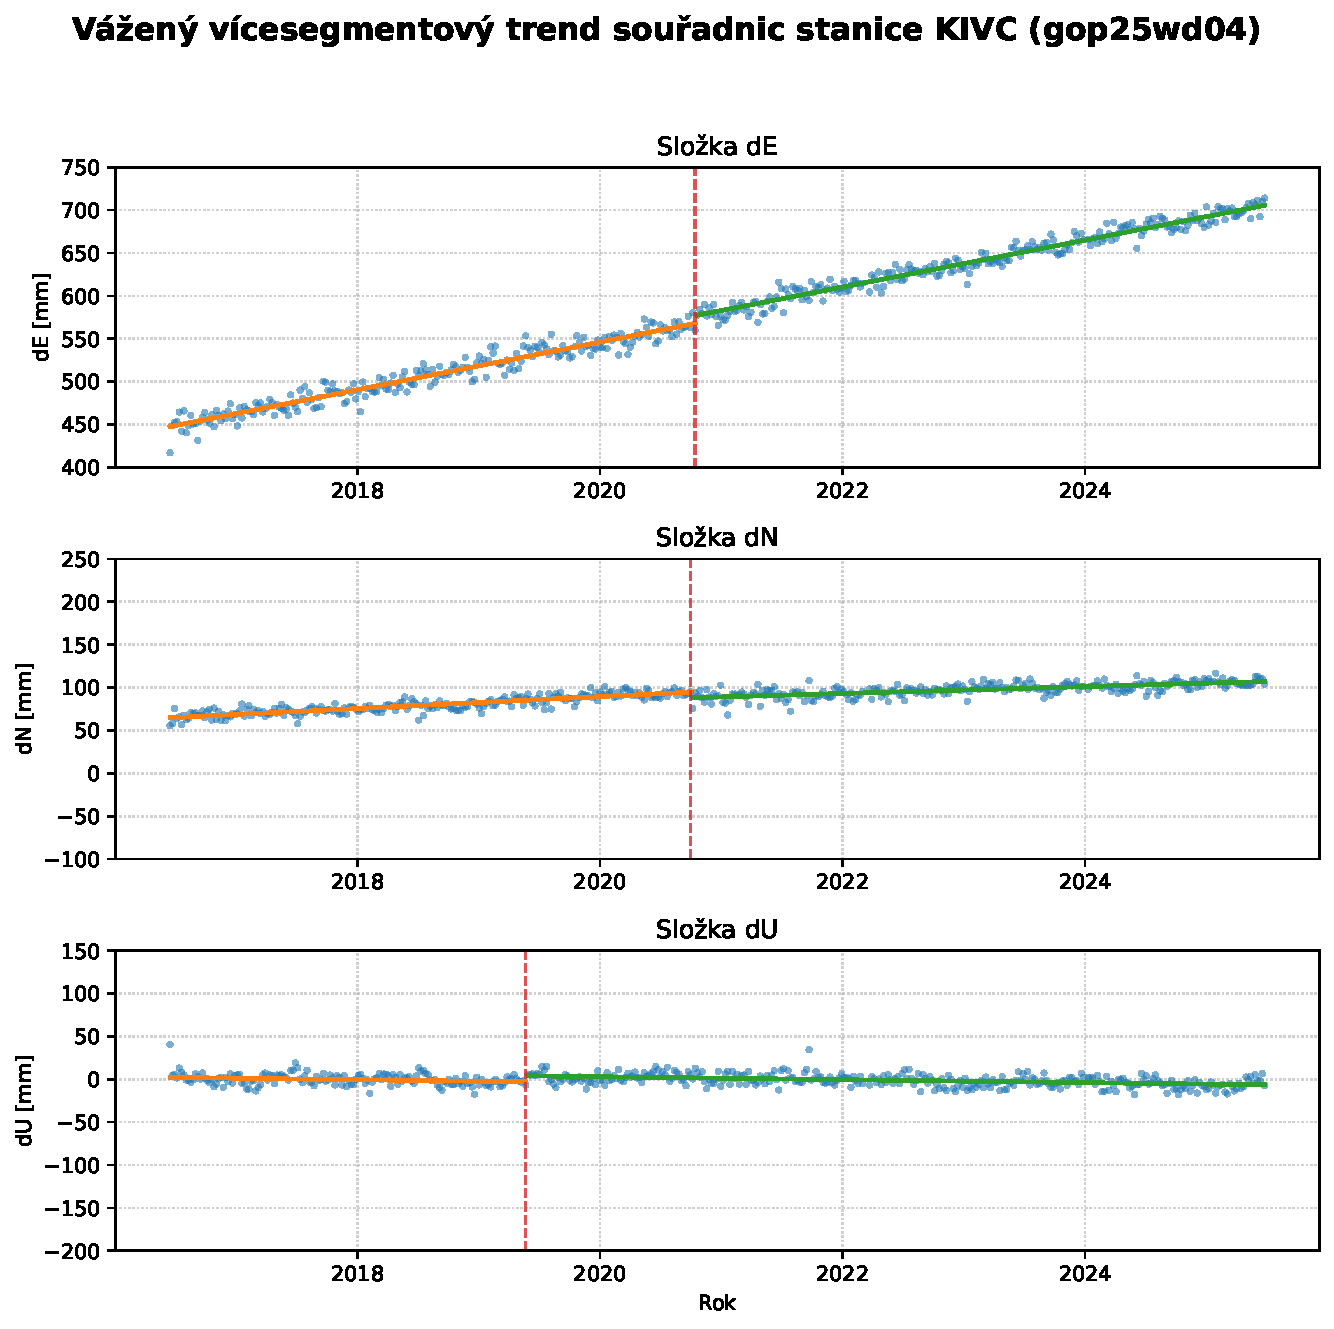
\includegraphics[width=1\textwidth]{images/results/stations/kivc/gop25wd04_stcd_kivc_trend_weighted_multiseg.pdf}
    \caption{Vážený model se zlomy pro souřadnice stanice KIVC}
    \label{fig:kivc_trend_breaks}
\end{figure}

\begin{table}[H]
\centering
\small
\caption{Identifikované zlomy v~časové řadě stanice KIVC.}
\label{tab:gop25wd04_stcd_kivc_trend_weighted_multiseg}
\begin{tabular}{lllllr}
\toprule
Složka & Počet segmentů & Zlomy & Trendy [mm/rok] & Skoky [mm] & $R^2$ \\
\midrule
dE & 2 & 14. 10. 2020 & 27.796, 27.359 & 9.125 & 0.989 \\
dN & 2 & 29. 9. 2020 & 6.952, 3.999 & -6.560 & 0.828 \\
dU & 2 & 22. 5. 2019 & -1.782, -1.725 & 7.062 & 0.166 \\
\bottomrule
\end{tabular}
\end{table}


Ve složkách dE a~dN byly identifikovány zlomy v~druhé polovině roku 2020. Ve složce dU byl nalezen dřívější zlom v~roce 2019. Zatímco ve složce dE se trend po zlomu změnil jen nepatrně, ve složce dN se trend změnil zhruba o~3~mm/rok.

Použití modelu se zlomy vede k~potlačení nenáhodného charakteru reziduí, jak je patrné z~obrázku~\ref{fig:kivc_res_breaks}. Snížení hodnot \zk{RMS} reziduí je uvedeno v~tabulce~\ref{tab:gop25wd04_stcd_kivc_residual_rms_comparison}.

\begin{table}[H]
\centering
\small
\caption{Porovnání RMS reziduí pro stanici KIVC}
\label{tab:gop25wd04_stcd_kivc_residual_rms_comparison}
\begin{tabular}{lrrr}
\toprule
Složka & Lineární [mm] & Se zlomy [mm] & Snížení [\%] \\
\midrule
dE & 8.45 & 8.15 & 3.5 \\
dN & 5.78 & 5.24 & 9.3 \\
dU & 6.75 & 6.46 & 4.4 \\
\bottomrule
\end{tabular}
\end{table}


\begin{figure}[H]
    \centering
    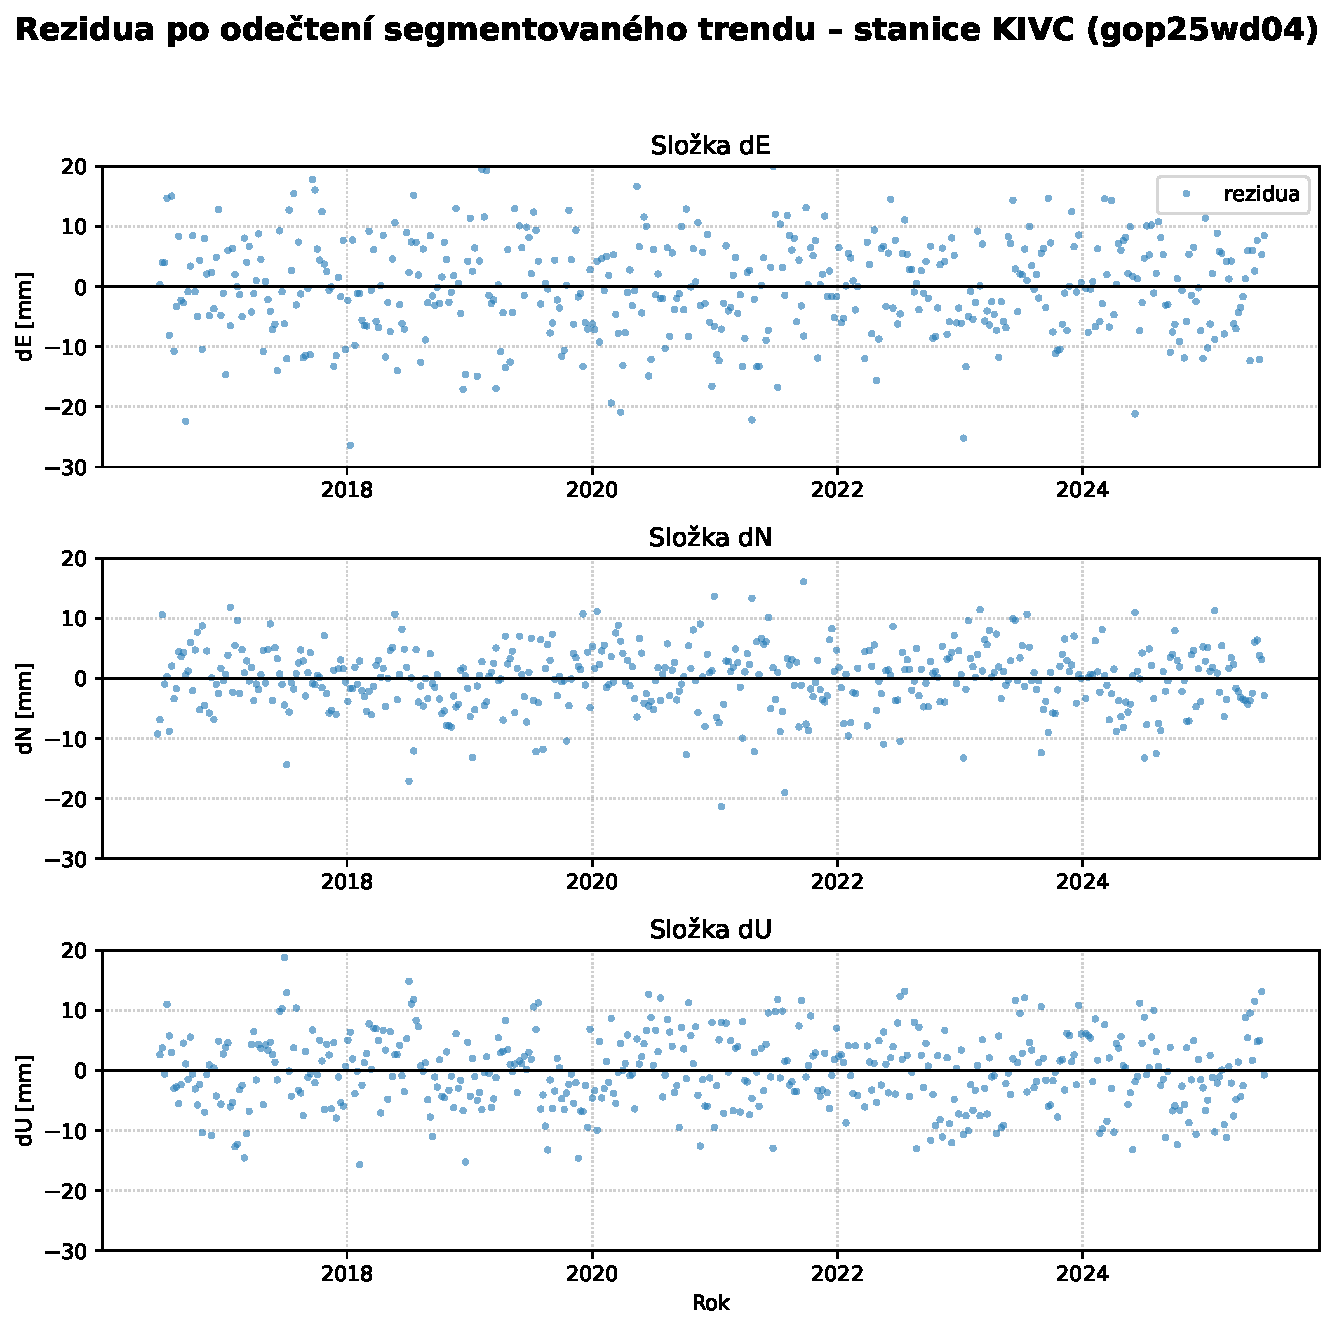
\includegraphics[width=1\textwidth]{images/results/stations/kivc/gop25wd04_stcd_kivc_residuals_weighted_multiseg.pdf}
    \caption{Rezidua po odečtení modelu se zlomy stanice KIVC}
    \label{fig:kivc_res_breaks}
\end{figure}

\subsubsection{Detekce diskontinuit}

Detekce diskontinuit byla provedena na reziduích po odečtení jednoduchého lineárního trendu, tedy před aplikací modelu se zlomy. Cílem bylo nezávisle ověřit, zda se v~časové řadě projeví diskontinuity naznačené modelem se zlomy. Použity byly dvě nezávislé metody: metoda dvou pohyblivých oken (obr.~\ref{fig:kivc_sliding_window}) a~metoda založená na analýze derivace vyhlazené časové řady (obr.~\ref{fig:kivc_lowess_derivative}).

\begin{figure}[H]
    \centering
    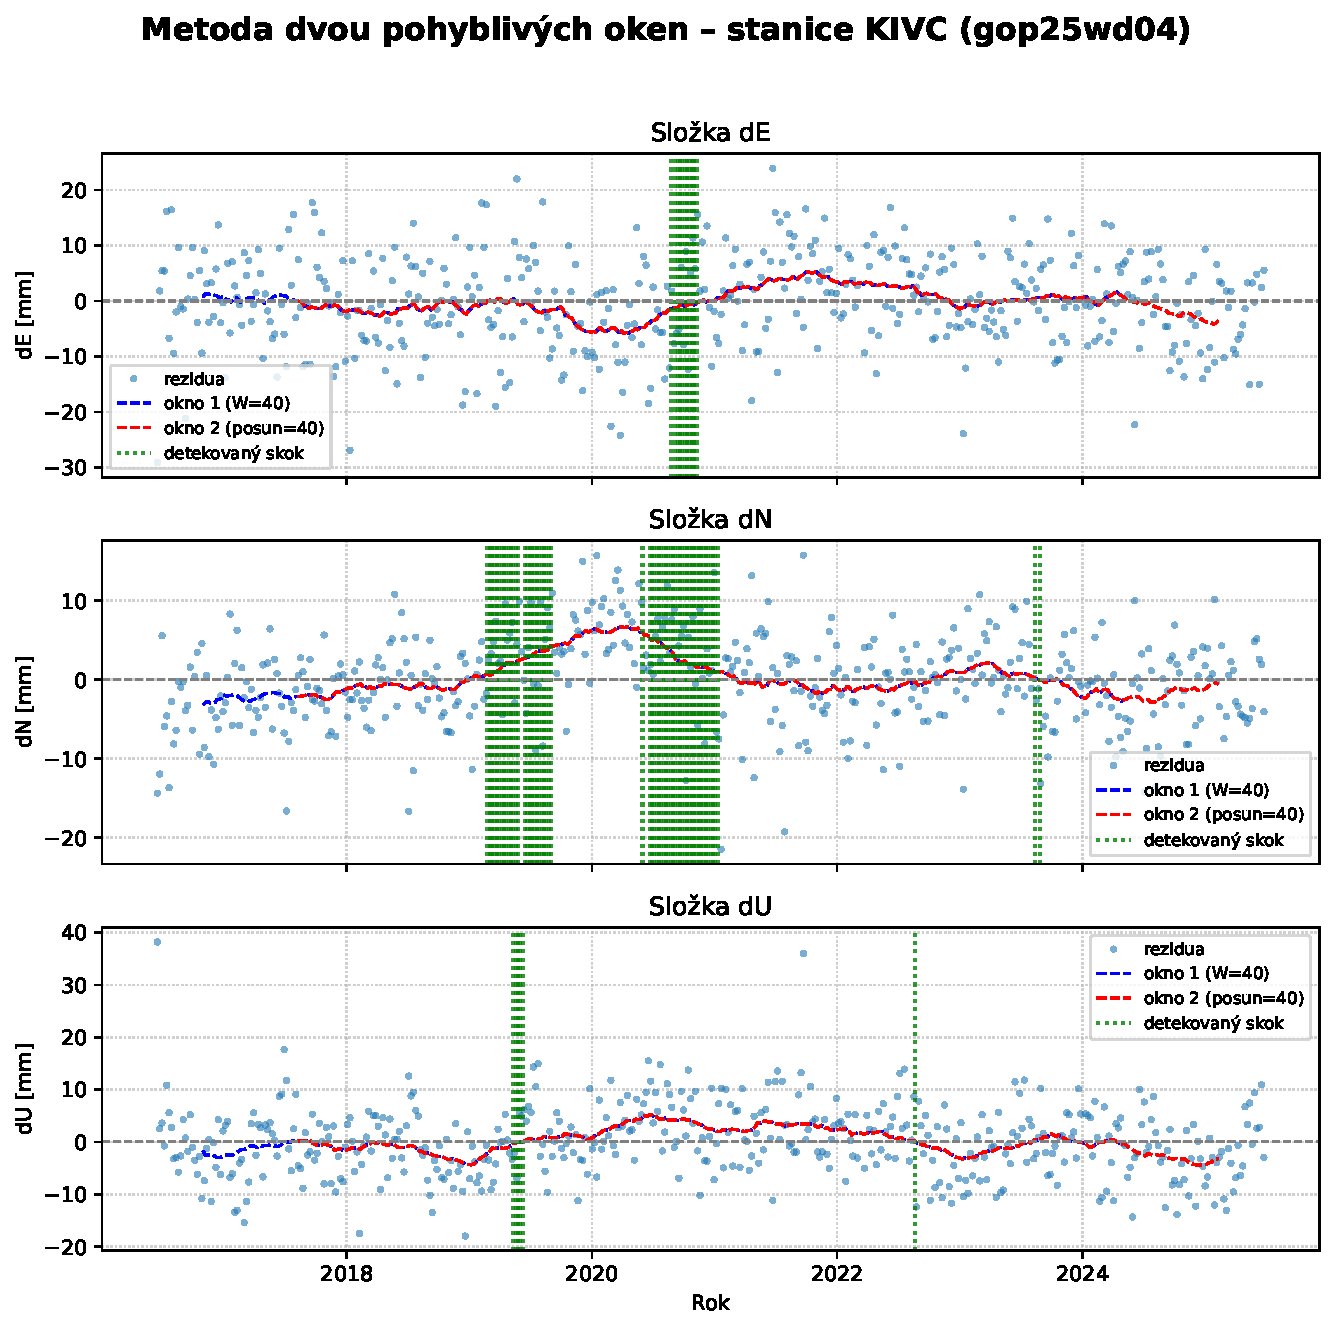
\includegraphics[width=1\textwidth]{images/results/stations/kivc/gop25wd04_stcd_kivc_detr_weighted_1seg_sliding_window.pdf}
    \caption{Detekce diskontinuit stanice KIVC pomocí dvou pohyblivých oken}
    \label{fig:kivc_sliding_window}
\end{figure}

\begin{figure}[H]
    \centering
    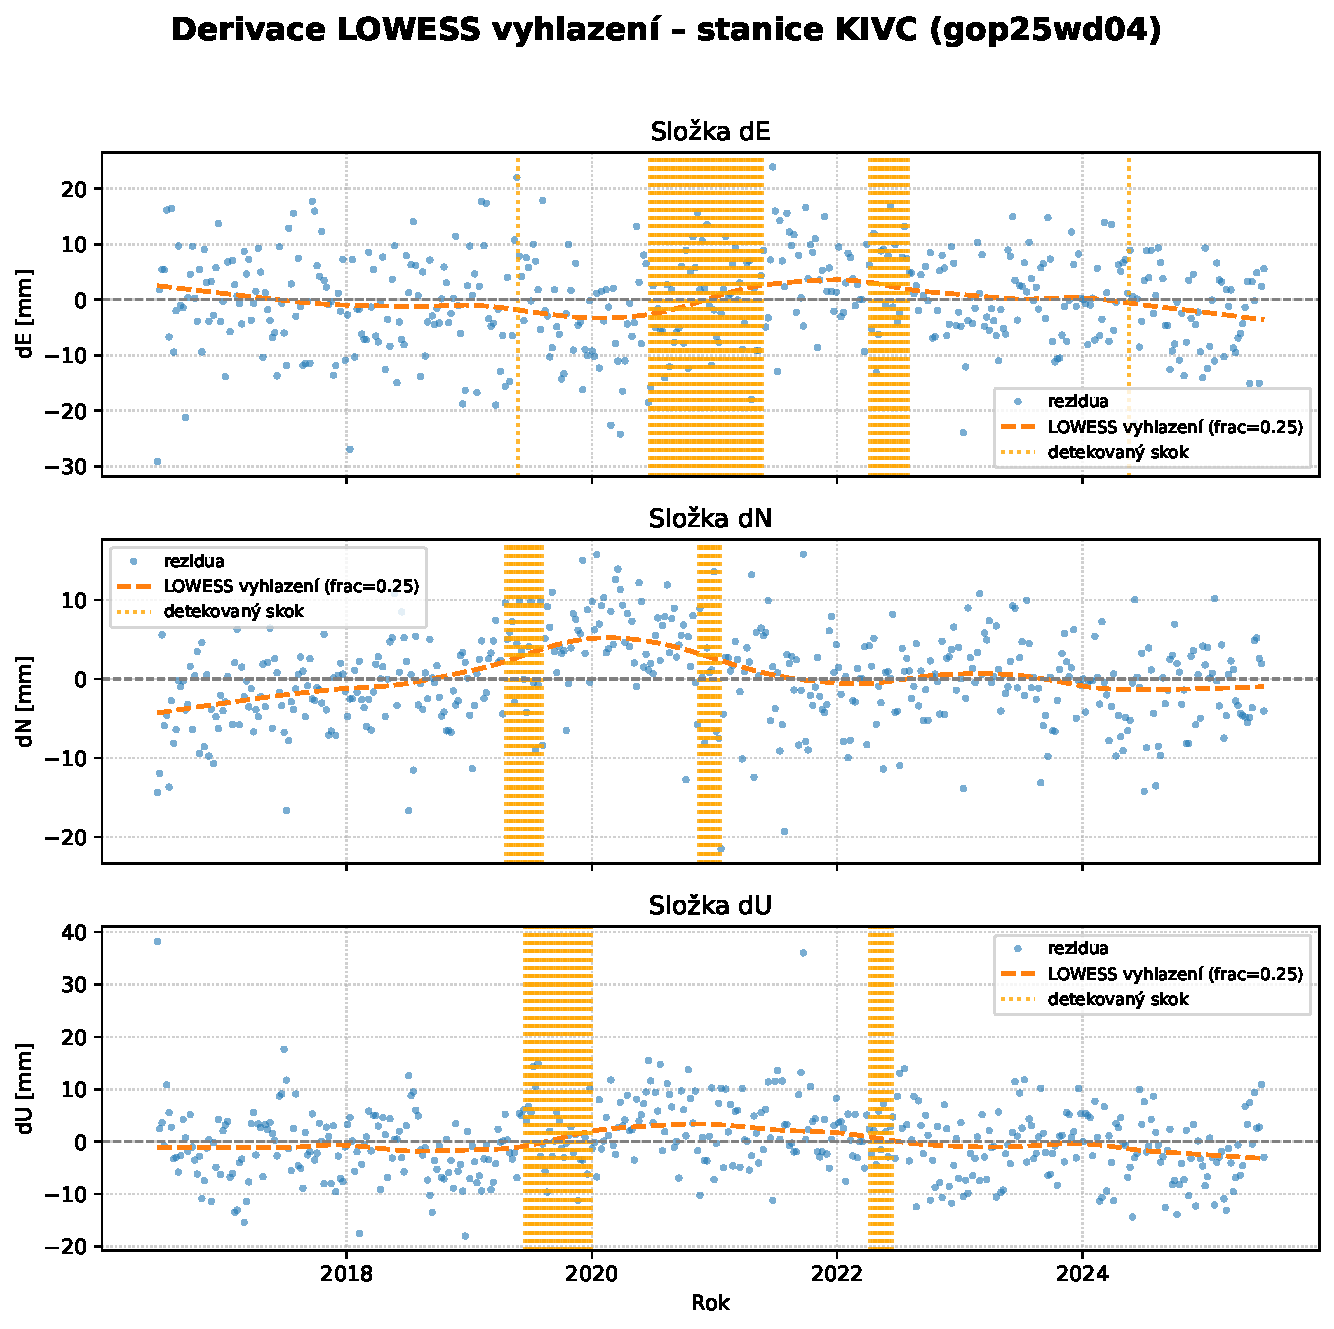
\includegraphics[width=1\textwidth]{images/results/stations/kivc/gop25wd04_stcd_kivc_detr_weighted_1seg_lowess_derivate.pdf}
    \caption{Detekce diskontinuit stanice KIVC pomocí analýzy derivace}
    \label{fig:kivc_lowess_derivative}
\end{figure}

Obě metody potvrzují, že časová řada stanice KIVC neobsahuje pouze náhodný rozptyl kolem lineárního trendu, ale také změny odpovídající diskontinuitám. Nejvýraznější shoda s~modelem se zlomy je patrná v~období kolem roku 2020, zejména v~horizontálních složkách dE a~dN. Ve složce dU jsou detekce méně jednoznačné.

\subsubsection{Spektrální analýza}

Spektrální analýza byla provedena na reziduích po odečtení lineárního trendu. Cílem bylo ověřit, zda nenáhodný charakter reziduí může být vysvětlen dominantní periodickou složkou. Na obrázku~\ref{fig:kivc_fft_periodogram} je uveden amplitudový periodogram získaný pomocí algoritmu \zkratka{FFT}.

\begin{figure}[H]
    \centering
    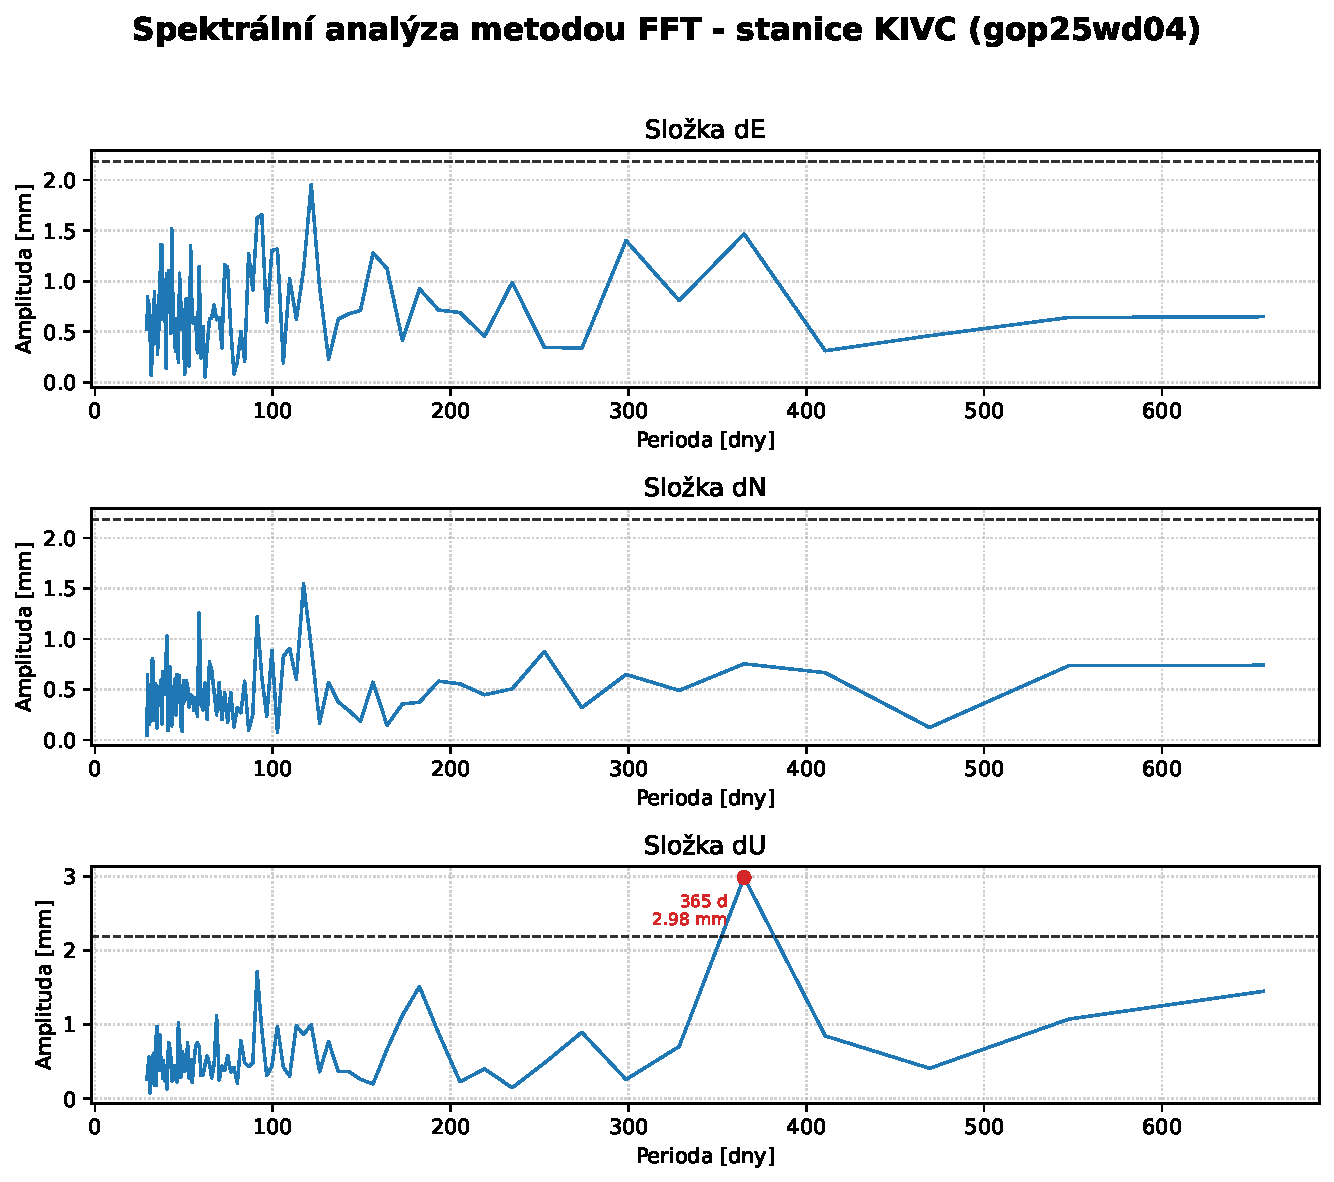
\includegraphics[width=1\textwidth]{images/results/stations/kivc/gop25wd04_stcd_kivc_detr_weighted_1seg_spectral_fft_periodogram.pdf}
    \caption{Periodogram reziduí stanice KIVC po odečtení lineárního trendu}
    \label{fig:kivc_fft_periodogram}
\end{figure}

Významná periodicita byla nalezena pouze ve vertikální složce dU, a to pro periodu přibližně 365~dní s~amplitudou přibližně 3{,}0~mm. Ve vodorovných složkách dE a~dN nebyla identifikována výrazná periodická složka.

Na základě nalezené periodicity byla rekonstruována periodická složka časové řady. Její průběh je znázorněn na obrázku~\ref{fig:kivc_fft_periodic_component}.

\begin{figure}[H]
    \centering
    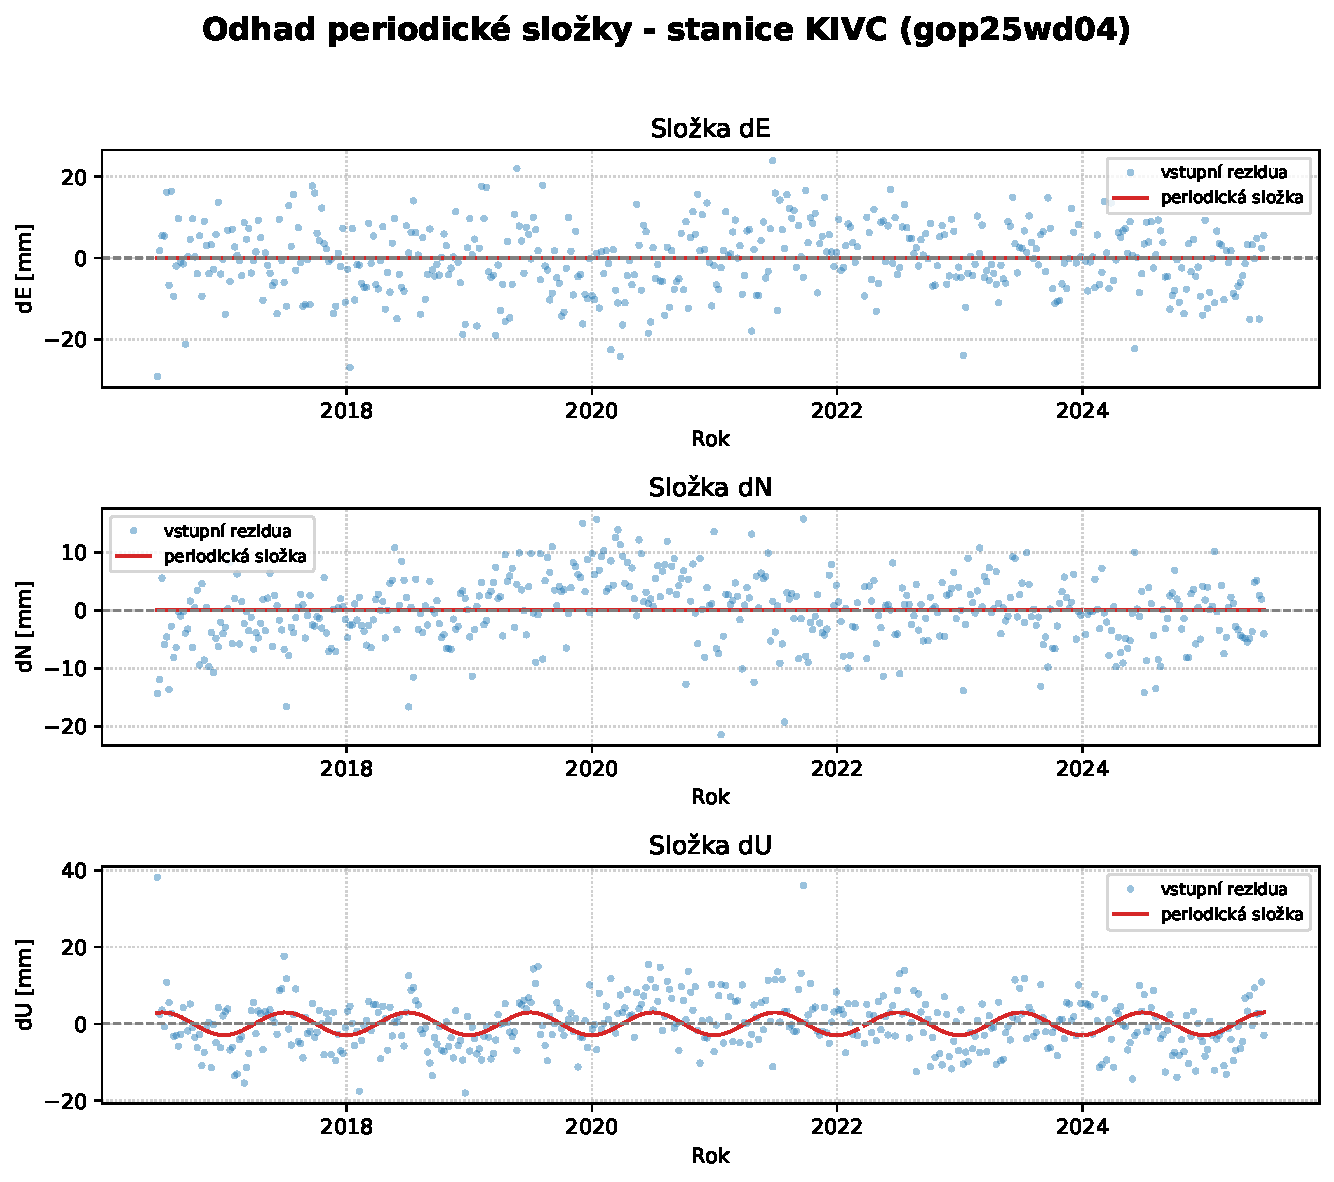
\includegraphics[width=\textwidth]{images/results/stations/kivc/gop25wd04_stcd_kivc_detr_weighted_1seg_spectral_fft_periodic_component.pdf}
    \caption{Rekonstruovaná periodická složka reziduí stanice KIVC}
    \label{fig:kivc_fft_periodic_component}
\end{figure}

Vliv odečtení periodické složky na rozptyl reziduí je uveden v~tabulce~\ref{tab:gop25wd04_stcd_kivc_detr_weighted_1seg_spectral_fft_variance_reduction}.

\begin{table}[htbp]
\caption{Snížení rozptylu po odstranění významných periodických složek určených metodou FFT pro stanici KIVC a řešení gop25wd04.}
\label{tab:gop25wd04_stcd_kivc_detr_weighted_1seg_spectral_fft_variance_reduction}
\begin{tabular}{llrrrr}
\toprule
Složka & Počet period & Rozptyl před [mm$^2$] & Rozptyl po [mm$^2$] & Snížení [mm$^2$] & Snížení [\%] \\
\midrule
dE & 0 & 71.396 & 71.396 & 0.000 & 0.0 \\
dN & 0 & 33.442 & 33.442 & 0.000 & 0.0 \\
dU & 1 & 45.664 & 41.221 & 4.443 & 9.7 \\
\bottomrule
\end{tabular}
\end{table}


Po odečtení roční periodické složky došlo ke snížení rozptylu vertikálních reziduí přibližně o~9{,}7~\%.

\subsubsection{Porovnání s~blízkými stanicemi}

Pro ověření, zda zjištěné změny mohou mít regionální charakter, byla stanice KIVC porovnána s~blízkými stanicemi ležícími na stejné litosférické desce. V~požadovaném časovém rozsahu byla dostupná stanice EVEB. Její časová řada vykazuje ve složkách dE a dN obdobné chování jako stanice KIVC, ve složce dU je výraznější periodická složka.

\subsubsection{Porovnání s~nezávislými řešeními}

Výsledky byly dále porovnány s~nezávislými kombinačními řešeními GRG, ESA a~GSC. Tato řešení vykazují podobné dlouhodobé chování časové řady, identické diskontinuity jako v~řešení GOP se však v~ostatních řešeních nevyskytují. Přesné epochy a velikosti diskontinuit se mezi řešeními liší a identické diskontinuity jako v~řešení GOP se v~ostatních řešeních nevyskytují.

\subsubsection{Interpretace}

Analýza stanice KIVC potvrzuje podezřelé chování indikované v~přehledu IDS, zejména změny ve vodorovných složkách kolem roku 2020. Ve složce dE byl nalezen skok přibližně $9{,}1$~mm bez výrazné změny trendu. Ve složce dN byl nalezen skok přibližně $-6{,}6$~mm a změna trendu přibližně o~3~mm/rok. Ve složce dU byl nalezen skok přibližně 7~mm v~roce 2019 bez výrazné změny trendu. Roční periodicita byla nalezena pouze ve vertikální složce a s~podezřelým chováním stanice zřejmě nemá přímou souvislost. Obdobné chování bylo částečně pozorováno také u~blízké stanice EVEB. Přímou souvislost se seismickou aktivitou ani s~přechodem z~\texttt{GOP67} na \texttt{GOP70} se nepodařilo prokázat.

\subsection{Souhrnné výsledky}
\label{sec:souhrn-casove-rady}

V~této části jsou shrnuty hlavní závěry analýzy všech vybraných stanic. Uvedeny jsou pouze výsledky, které mají význam pro interpretaci podezřelého chování stanic. Kompletní grafické výstupy, odhady trendů, detekce diskontinuit a porovnání s~nezávislými řešeními jsou uvedeny v~příloze~report\_stations.pdf.

\subsubsection{KIVC -- Kitab, Uzbekistán}

U~stanice KIVC bylo potvrzeno podezřelé chování indikované na přelomu let 2019 a 2020. Nejvýrazněji se projevilo ve vodorovných složkách, kde byl ve složce dE identifikován skok přibližně $9{,}1$~mm a ve složce dN skok přibližně \(-6{,}6\)~mm doprovázený změnou trendu přibližně o~3~mm/rok. Ve vertikální složce dU byl nalezen skok přibližně 7~mm v~roce 2019. Obdobné chování bylo pozorováno také u~blízké stanice EVEB, zatímco v~nezávislých řešeních GRG, ESA a GSC se identické diskontinuity nevyskytují. Příčinu se nepodařilo jedno\-značně určit. Seismická aktivita ani přechod z~\texttt{GOP67} na \texttt{GOP70} nebyly potvrzeny jako pravděpodobné vysvětlení.

\subsubsection{JIWC -- Jiufeng, Čína}

U~stanice JIWC se podezřelé chování projevuje především ve vertikální složce dU po roce 2020. Po přerušení časové řady v~roce 2019 se rezidua ve složce dU výrazně rozptylují a průběh časové řady se spíše pozvolna vlní, než že by obsahoval jeden jednoznačný skok. Podobný charakter má tato složka také v~nezávislých řešeních GRG, ESA a GSC, takže se pravděpodobně nejedná pouze o~artefakt řešení GOP. Jednoznačnou příčinu se nepodařilo určit. Seismická aktivita ani zjištěné periodické složky pozorované chování dostatečně nevysvětlují.

\subsubsection{LICB -- Libreville, Gabon}

U~stanice LICB byl ve složce dU nalezen v~roce 2016 skok přibližně $18{,}9$~mm. Ve složkách dE a~dN byly identifikovány také další diskontinuity a ve složce dE byly nalezeny výrazné periodické složky, včetně periody přibližně $118$~dní odpovídající beta-prime periodě družic typu Jason a~Sentinel-6A. Blízké stanice HEMB a~SARC obdobné chování v~okolí roku~2016 nevykazují. Řešení ESA vykazuje podobné nestandardní chování jako řešení GOP, zatímco řešení GRG a~GSC se v~nalezených diskontinuitách a periodicitách liší, vykazují však také určité nestandardní chování. Vzhledem k~časové blízkosti začátku mise Sentinel-3A se jako možné vysvětlení nabízí změna ve zpracování související s~přidáním této družice.

\subsubsection{SARC -- Sal, Kapverdy}

U~stanice SARC bylo potvrzeno podezřelé chování ve složce dE na konci roku 2020. Projevuje se výrazným skokem přibližně \(-33~\mathrm{mm}\), zatímco změna trendu je pouze malá. Podobný skok byl nalezen také u~stanice PDOC ležící na stejné tektonické desce, v~nezávislých řešeních se však obdobné chování objevuje jen částečně. Původ skoku se nepodařilo jedno\-značně určit. Časově však odpovídá přechodu z~\texttt{GOP67} na \texttt{GOP70}, a proto nelze vyloučit souvislost se změnou zpracování.

\subsubsection{STKC -- St.~John's, Kanada}

U~stanice STKC bylo potvrzeno podezřelé chování především ve složce dE na přelomu let 2020 a~2021, kde byl identifikován skok přibližně $-16{,}3$~mm s~poměrně malou změnou trendu. Rezidua však naznačují spíše pozvolný nelineární výkyv než jednoduchý jednorázový skok. Ve složce dN byly nalezeny také další méně výrazné diskontinuity, zatímco ve složce dU byl preferován prostý lineární model bez skoku. Ve žádné ze složek nebyla nalezena výrazná periodická složka. Okolní stanice ani nezávislá řešení GRG, ESA a~GSC obdobné chování nevykazují. Výsledek proto spíše ukazuje na artefakt zpracování dat než na regionální geodynamický jev.

\subsubsection{CADB -- Cachoeira, Brazílie}

U~stanice CADB byla potvrzena indikovaná diskontinuita ve vertikální složce dU, kde byl nalezen skok přibližně 27{,}5~mm. Menší skoky byly nalezeny také v~letech 2016 a~2020. Diskontinuity byly identifikovány i~ve složkách dE a~dN, přičemž ve složce dE byl v~roce 2016 nalezen skok dosahující přibližně 57~mm. Blízká stanice KRWB ani nezávislá řešení GRG, ESA a~GSC obdobné chování nevykazují, i~když i~u~nich lze také pozorovat nestandardní chování. Nalezené diskontinuity se nepodařilo jedno\-značně vysvětlit. Skoky v~roce 2016 přibližně odpovídají začátku mise Sentinel-3A, zatímco skoky v~roce 2018 zhruba odpovídají začátku mise Sentinel-3B. Interpretaci výsledků navíc komplikuje poloha stanice CADB v~oblasti Jihoatlantické magnetické anomálie. V~důsledku toho se při zpracování aplikují specifické kompenzační strategie, které se mohou mezi jednotlivými analytickými centry lišit.

\subsubsection{THUB -- Thule, Grónsko}

U~stanice THUB bylo potvrzeno podezřelé chování ve složkách dE a~dN, kde byly identifikovány menší diskontinuity a~změny trendu. Nejvýraznější změna byla nalezena ve složce dN na přelomu let 2020 a~2021. Vertikální složka dU zároveň vykazuje výrazné glacioizostatické zdvihání typické pro oblast Grónska. Ve složce dN byla nalezena přibližně roční periodická složka a~ve složce dU perioda přibližně 118~dní, odpovídající beta-prime periodě. Okolní stanice ani nezávislá řešení obdobné chování nevykazují. Nalezené diskontinuity časově přibližně odpovídají přechodu z~\texttt{GOP67} na \texttt{GOP70}, a~proto nelze vyloučit souvislost se změnou zpracování dat.

\subsubsection{MSPB -- Mount Stromlo, Austrálie}

U~stanice MSPB byla ve složce dN nalezena změna kolem roku 2021. Formálně ji lze popsat skokem přibližně 9{,}0~mm, průběhem však spíše odpovídá krátkodobému výkyvu. Ve složce dE byla spektrální analýzou nalezena periodická složka s~periodou přibližně 118~dní a~amplitudou okolo 2{,}2~mm. Tato periodicita dobře odpovídá orbitální beta-prime periodě typické pro družice typu Jason a~Sentinel-6A, související se změnami úhlu mezi rovinou dráhy družice a~směrem Slunce--družice. Odstranění této periodicity však vedlo pouze k~malému snížení rozptylu a~nevysvětluje nalezený výkyv ve složce dN. Blízké stanice NOXB/NOXC a~YASB ani nezávislá řešení GRG, ESA a~GSC podobné chování nevykazují. Výsledek proto spíše naznačuje lokální artefakt v~řešení GOP než fyzikální změnu stanice.

\subsubsection{KRWB -- Kourou, Francouzská Guyana}

U~stanice KRWB byly nalezeny diskontinuity a~změny trendu ve složkách dE a~dU, nejvýrazněji ve složce dE před rokem~2020. Ve složce dN nebyla nalezena statisticky přesvědčivá diskontinuita, byla zde však identifikována výrazná roční periodicita. Spektrální analýza zároveň ukázala přítomnost periodických složek i~v~ostatních složkách, včetně periody přibližně 118~dní ve složce dE. Srovnání s~blízkou stanicí CADB neukázalo identické chování, přestože i~tato stanice vykazuje nestandardní chování. Řešení GOP a~GRG jsou si v~tomto případě podobná, zatímco ESA a~GSC se odlišují. Jednoznačnou příčinu podezřelého chování se nepodařilo určit.

\clearpage
\section{Dráhy družic}
\label{sec:vysledky-drahy}

Analyzovány byly přesné dráhy družic vybavených přijímačem systému \zkratka{DORIS} za~prvních 30~dní roku 2024. Cílem bylo porovnat řešení drah poskytované analytickým centrem GOP s~řešením \zk{SSA} a~kvantifikovat rozdíly mezi těmito řešeními. Porovnání bylo provedeno dvěma způsoby -- matematickou interpolací (Hermitova interpolace implementovaná v~jazyce Python), která umožňuje převod drah na společné epochy, a~dynamickou parametrizací dráhy v~softwaru \zkratka{BSW}. Nakonec byly srovnány oba tyto přístupy, aby byl posouzen vliv zvolené metody na výsledné rozdíly. Analyzovány byly družice:


\begin{itemize}
\item \textbf{srl} -- SARAL
\item \textbf{cs2} -- CryoSat-2
\item \textbf{h2c} -- HY-2C
\item \textbf{h2d} -- HY-2D
\item \textbf{ja3} -- Jason-3
\item \textbf{s3a} -- Sentinel-3A
\item \textbf{s3b} -- Sentinel-3B
\item \textbf{s6a} -- Sentinel-6A
\end{itemize}

Rozdíly drah byly vyhodnoceny v~lokálním systému \zk{RTN} a~pro jednotlivé dny vyčísleny pomocí průměru, \zkratka{RMS} a~\zkratka{RMS}0 v~jednotlivých složkách \zk{RTN} a~celkově jako 3D~RMS.
\subsection{Ukázka analýzy: družice SARAL}

Kompletní analýza je v~textu práce předvedena na~družici \zkratka{SARAL}. Detailní výsledky pro~všechny analyzované družice jsou uvedeny v~přílohách.

\subsubsection{Porovnání pomocí interpolace}

Rozdíly drah \zk{GOP} a \zk{SSA} byly nejprve vyhodnoceny pomocí Hermitovy interpolace, přičemž známé polohy družice byly interpolovány na~společné epochy, aby bylo možné obě řešení přímo porovnat.

\paragraph{Průběh rozdílů v~rámci jednoho dne}\leavevmode\\
Na obrázku~\ref{fig:srl_herm_diff_doy001} je zobrazen průběh rozdílů \zk{GOP}\,--\,\zk{SSA} ve složkách RTN pro den 1.\,1.\,2024, který byl zvolen jako reprezentativní ukázka.

\begin{figure}[H]
    \centering
    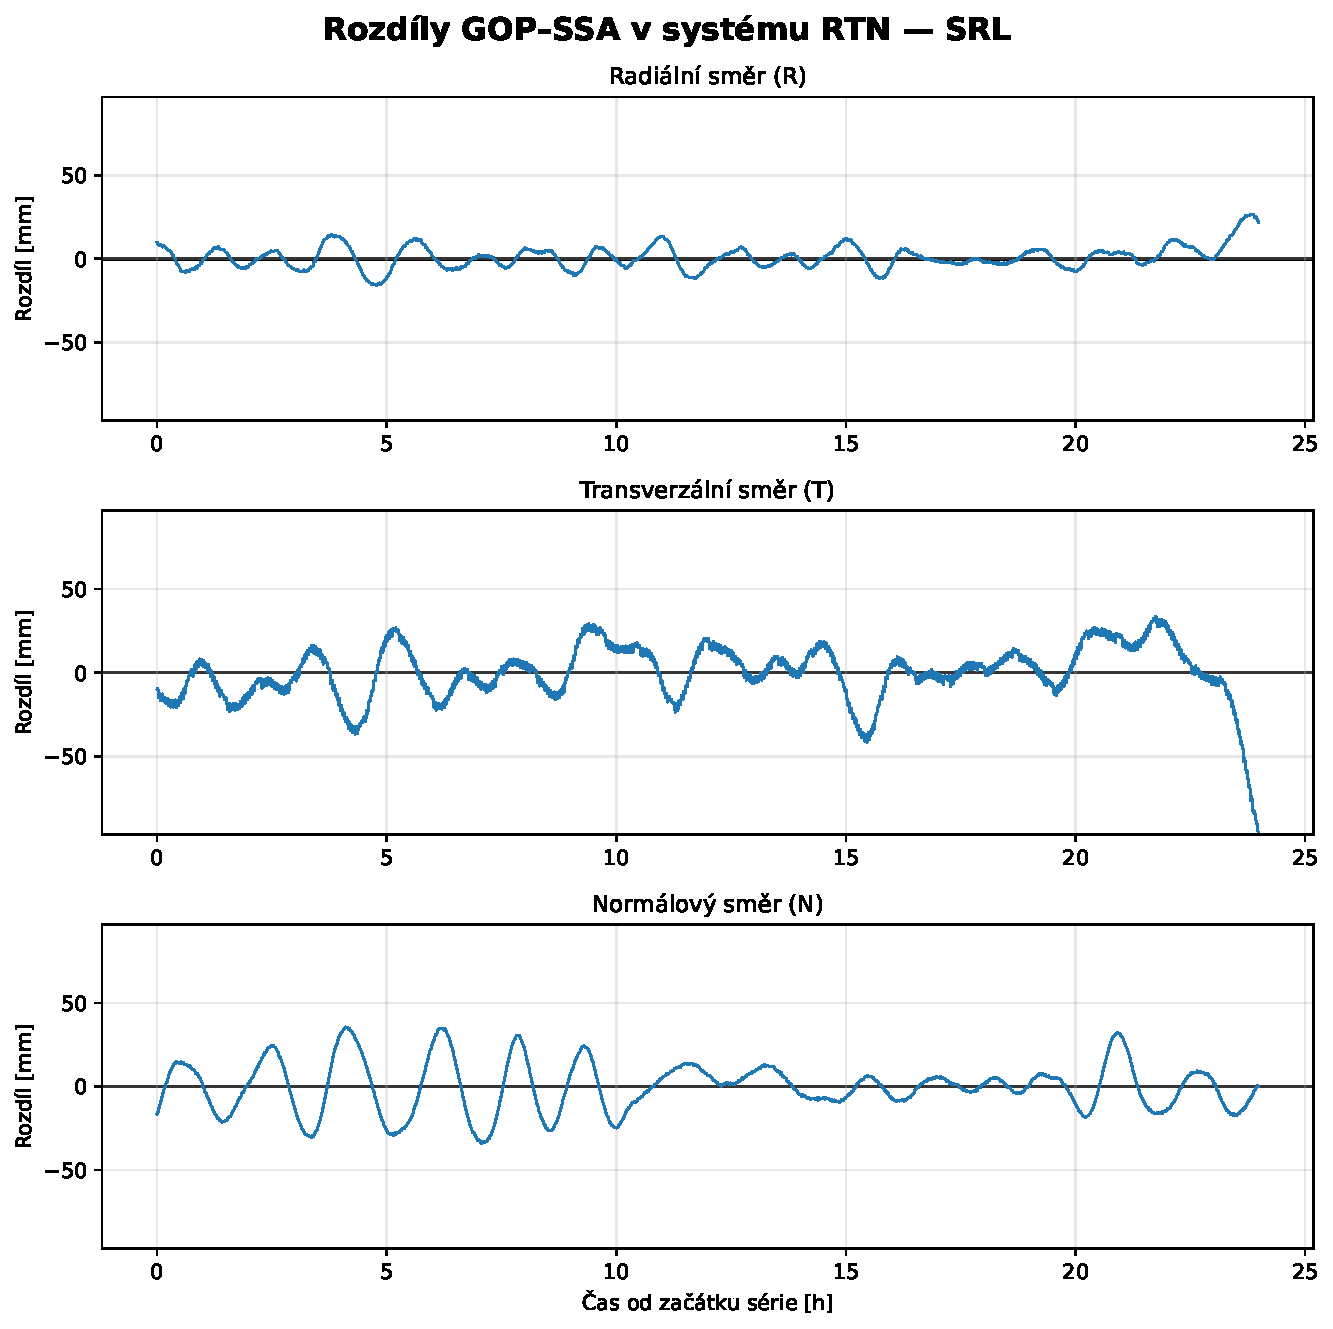
\includegraphics[width=1\textwidth]{images/results/satellites/hermite/srl/gop_vs_ssa_srl_doy001_rtn_differences.pdf}
    \caption{Průběh rozdílů \zk{GOP}\,--\,\zk{SSA} v~systému RTN družice SARAL}
    \label{fig:srl_herm_diff_doy001}
\end{figure}

Z~obrázku~\ref{fig:srl_herm_diff_doy001} je patrné, že rozdíly mezi řešeními se v~jednotlivých složkách chovají odlišně. Radiální složka~R se pohybuje přibližně v~rozmezí $\pm$\,20\,mm bez výraznějšího trendu v~průběhu dne. Transverzální složka~T dosahuje přibližně $\pm$\,40\,mm, avšak ke konci analyzovaného dne rozdíl mezi oběma řešeními výrazně narůstá. Normálová složka~N vykazuje odchylky přibližně $\pm$\,50\,mm a~její průběh vykazuje známky systematické struktury.

Pro posouzení rozložení rozdílů jsou na~obrázku~\ref{fig:srl_herm_hist_doy001} uvedeny histogramy pro jednotlivé složky systému \zk{RTN}.

\begin{figure}[H]
    \centering
    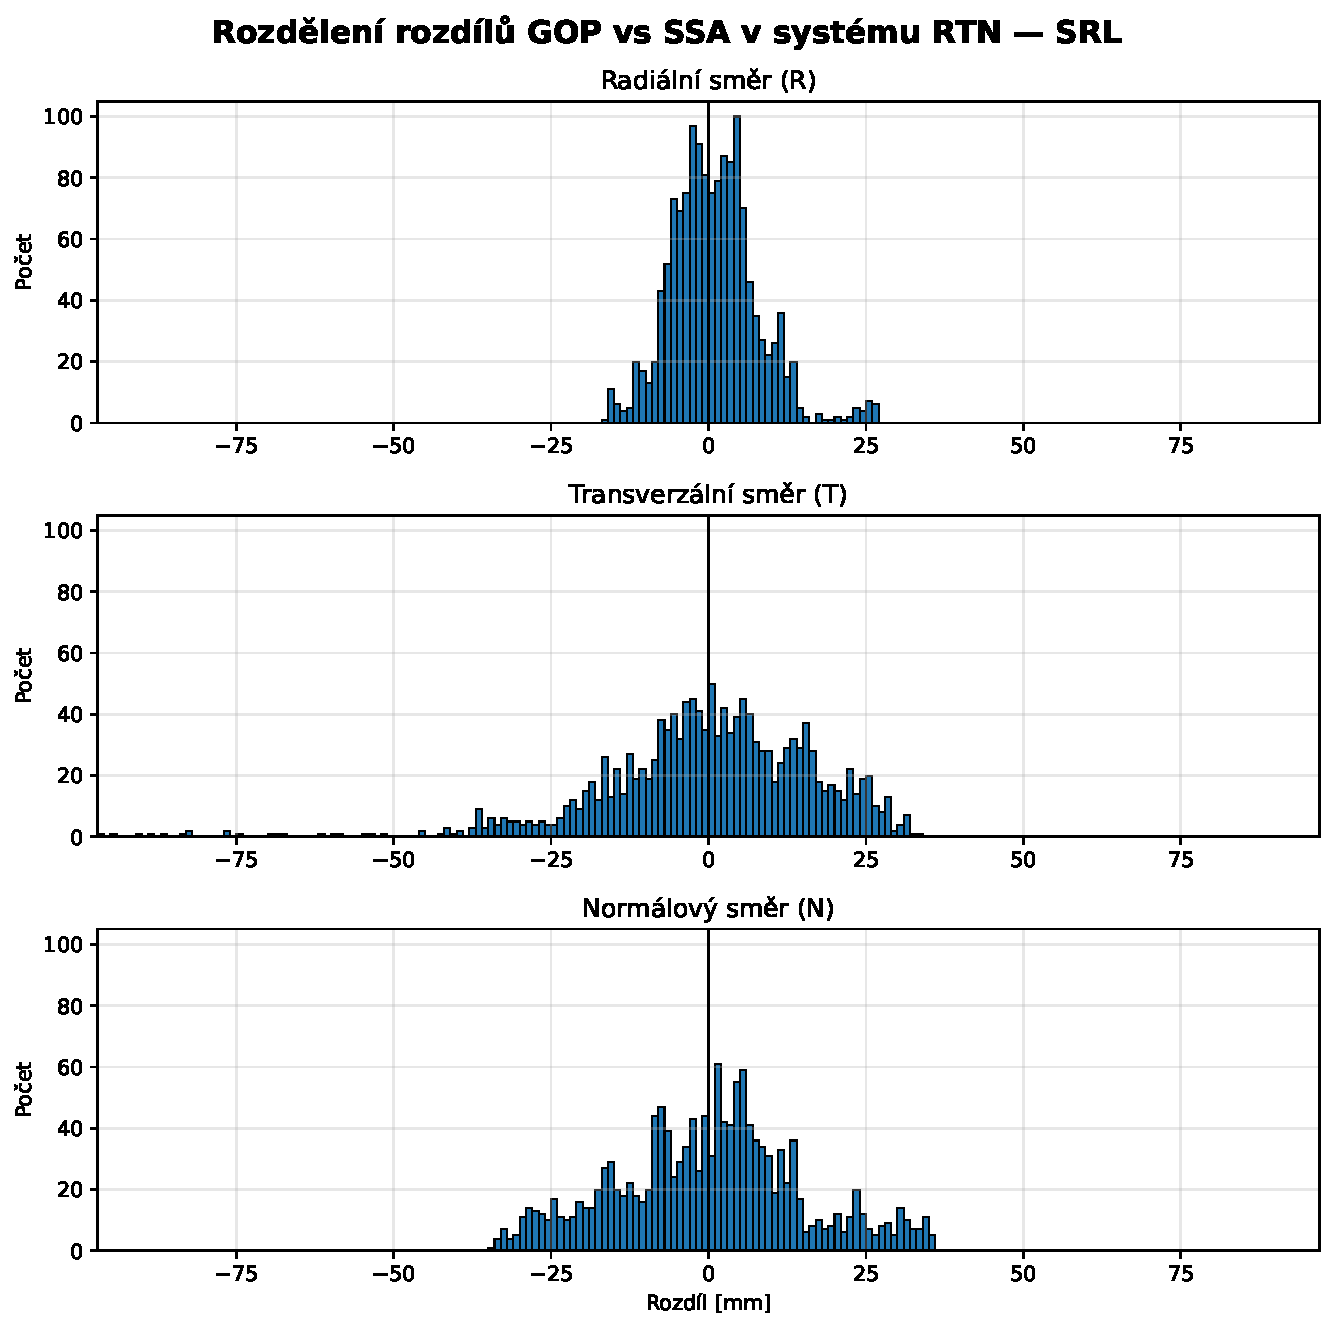
\includegraphics[width=1\textwidth]{images/results/satellites/hermite/srl/gop_vs_ssa_srl_doy001_rtn_histogram.pdf}
    \caption{Histogramy rozdílů \zk{GOP}\,--\,\zk{SSA} v~systému \zk{RTN} družice SARAL}
    \label{fig:srl_herm_hist_doy001}
\end{figure}

Z~histogramů vyplývá, že rozdíly jsou ve všech složkách soustředěny kolem nulové hodnoty a~není patrný výrazný systematický posun mezi oběma řešeními. Rozdělení se v~jednotlivých složkách liší šířkou i~tvarem. Radiální složka~R vykazuje nejužší a~nejsymetričtější rozdělení. Transverzální složka~T je výrazně širší a~mírně asymetrická s~přesahem do~záporných hodnot, který odpovídá nárůstu rozdílů ke konci analyzovaného dne. Normálová složka~N má plošší a~rovnoměrnější rozdělení, což odpovídá většímu rozptylu.

\paragraph{Spektrální analýza rozdílů}\leavevmode\\
Pro identifikaci periodicit v~rozdílech obou řešení byl vypočten Lomb--Scargleův periodogram, přičemž na~obrázku~\ref{fig:srl_herm_pg_doy001} jsou znázorněny periodogramy pro jednotlivé složky systému \zk{RTN}.

\begin{figure}[H]
    \centering
    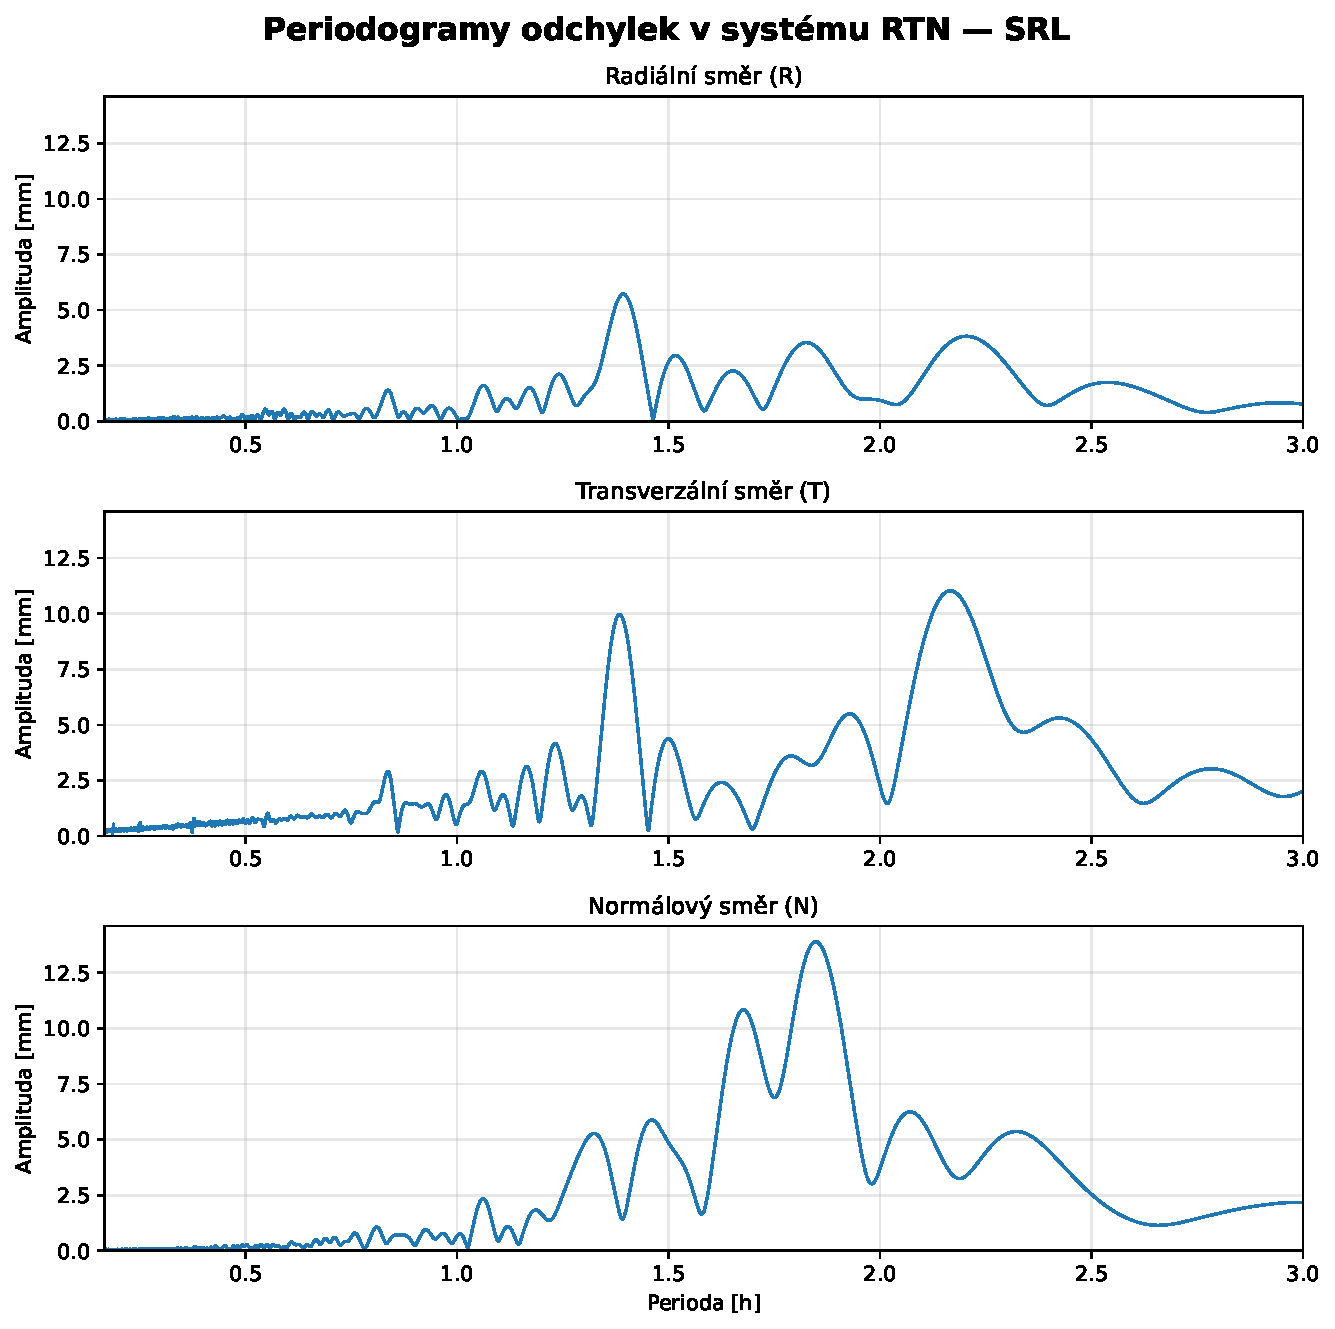
\includegraphics[width=1\textwidth]{images/results/satellites/hermite/srl/gop_vs_ssa_srl_doy001_rtn_periodograms_lomb_scargle.pdf}
    \caption{Periodogram rozdílů \zk{GOP}\,--\,\zk{SSA} v~systému \zk{RTN} družice SARAL}
    \label{fig:srl_herm_pg_doy001}
\end{figure}

Z~periodogramů je patrné, že v~normálové složce~N jsou přítomny výrazné vrcholy v~oblasti period přibližně 80--110\,min, tedy v~okolí oběžné doby družice \zkratka{SARAL}. Podobné vrcholy jsou patrné také v~transverzální složce~T, zatímco v~radiální složce~R jsou amplitudy výrazně nižší.

\paragraph{Dlouhodobá stabilita rozdílů}\leavevmode\\
Pro posouzení časové stability jsou na~obrázku~\ref{fig:srl_herm_rms_daily} znázorněny denní hodnoty \zkratka{RMS} rozdílů ve složkách \zk{RTN} a~celkové 3D~\zkratka{RMS} v~průběhu prvních 30~dnů roku 2024.

\begin{figure}[H]
    \centering
    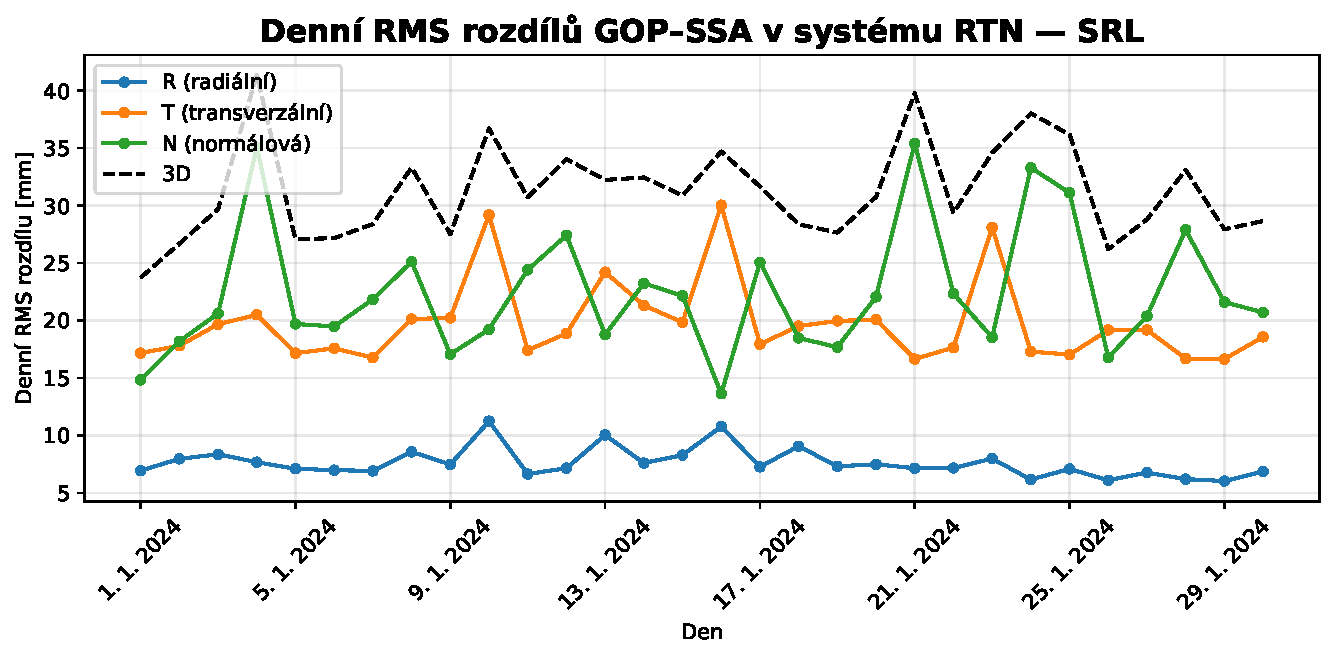
\includegraphics[width=1\textwidth]{images/results/satellites/hermite/srl/gop_vs_ssa_srl_doy001-doy030_daily_rtn_3d_rms.pdf}
    \caption{Denní RMS rozdílů \zk{GOP}\,--\,\zk{SSA} získané Hermitovou interpolací}
    \label{fig:srl_herm_rms_daily}
\end{figure}

Z~grafu je patrné, že hodnoty \zkratka{RMS} v~radiální složce jsou v~celém analyzovaném období stabilní a~pohybují se přibližně v~rozmezí 6--11\,mm, průměrně kolem 8\,mm. Transverzální složka~T dosahuje hodnot zhruba 16--30\,mm (průměrně $\sim$20\,mm), zatímco normálová složka~N se pohybuje v~rozsahu 14--35\,mm (průměrně $\sim$25\,mm) a~vykazuje největší variabilitu mezi jednotlivými dny. Celkové 3D~\zkratka{RMS} se pohybuje průměrně kolem 33\,mm.

\subsubsection{Porovnání pomocí dynamické parametrizace}

Druhý přístup vychází z~dynamické parametrizace v~\zkratka{BSW}. Dráhy ve formátu SP3 jsou v~modulu \texttt{ORBGEN} využity k~získání dynamické reprezentace dráhy. Rozdíly jsou určeny jako rozdíly polohy těchto drah ve společných epochách.

\paragraph{Průběh rozdílů v~rámci jednoho dne}\leavevmode\\
Na obrázku~\ref{fig:srl_bsw_diff_doy001} je znázorněn průběh rozdílů \zk{GOP}\,--\,\zk{SSA} ve složkách \zk{RTN} získaných pomocí dynamické parametrizace v~softwaru \zkratka{BSW}.

\begin{figure}[H]
    \centering
    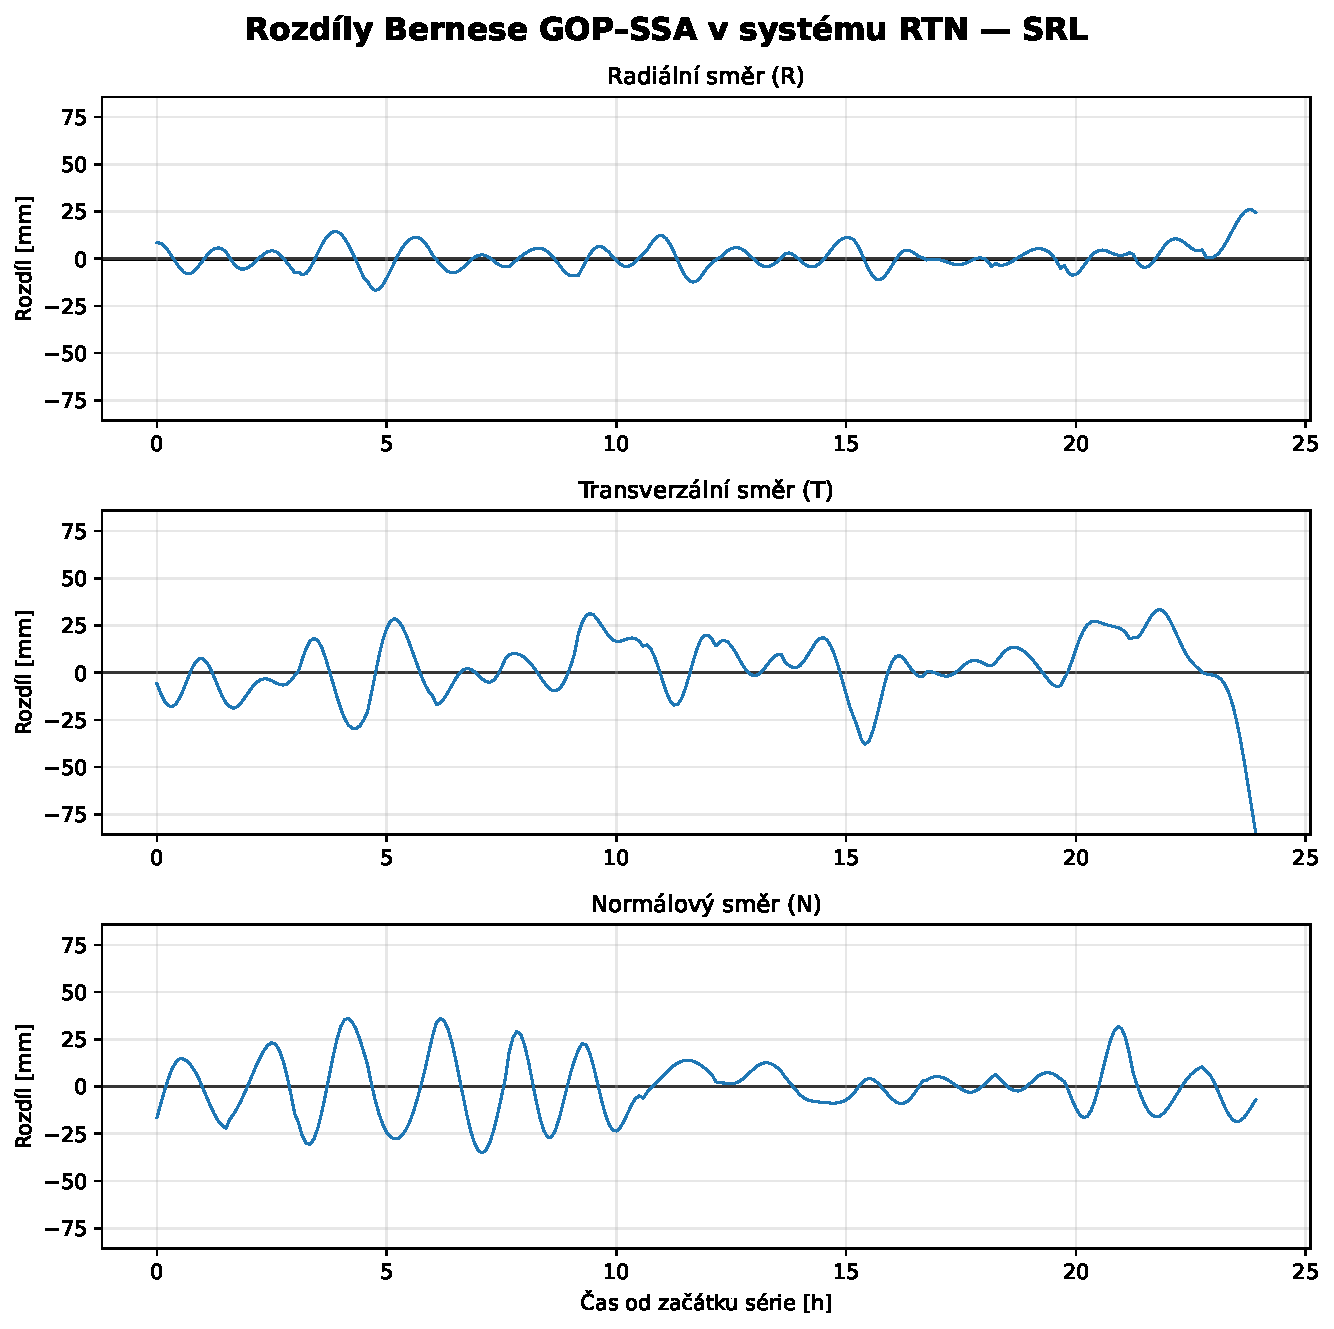
\includegraphics[width=1\textwidth]{images/results/satellites/bernese/sa/sa_ZAZG_doy001_rtn_differences.pdf}
    \caption{Průběh rozdílů \zk{GOP}\,--\,\zk{SSA} získaných dynamickou parametrizací}
    \label{fig:srl_bsw_diff_doy001}
\end{figure}

Průběh rozdílů je ve všech třech složkách prakticky totožný s~výsledky Hermitovy interpolace. Histogramy a~periodogram rozdílů jsou téměř shodné s~výsledky interpolační metody a~jsou uvedeny v~příloze.

\paragraph{Stabilita rozdílů v~čase}\leavevmode\\
Na obrázku~\ref{fig:srl_bsw_rms_daily} jsou znázorněny denní hodnoty \zkratka{RMS} rozdílů \zk{GOP}\,--\,\zk{SSA} ve složkách \zk{RTN} a~celkové 3D~\zkratka{RMS} v~průběhu prvních 30~dní roku 2024.

\begin{figure}[H]
    \centering
    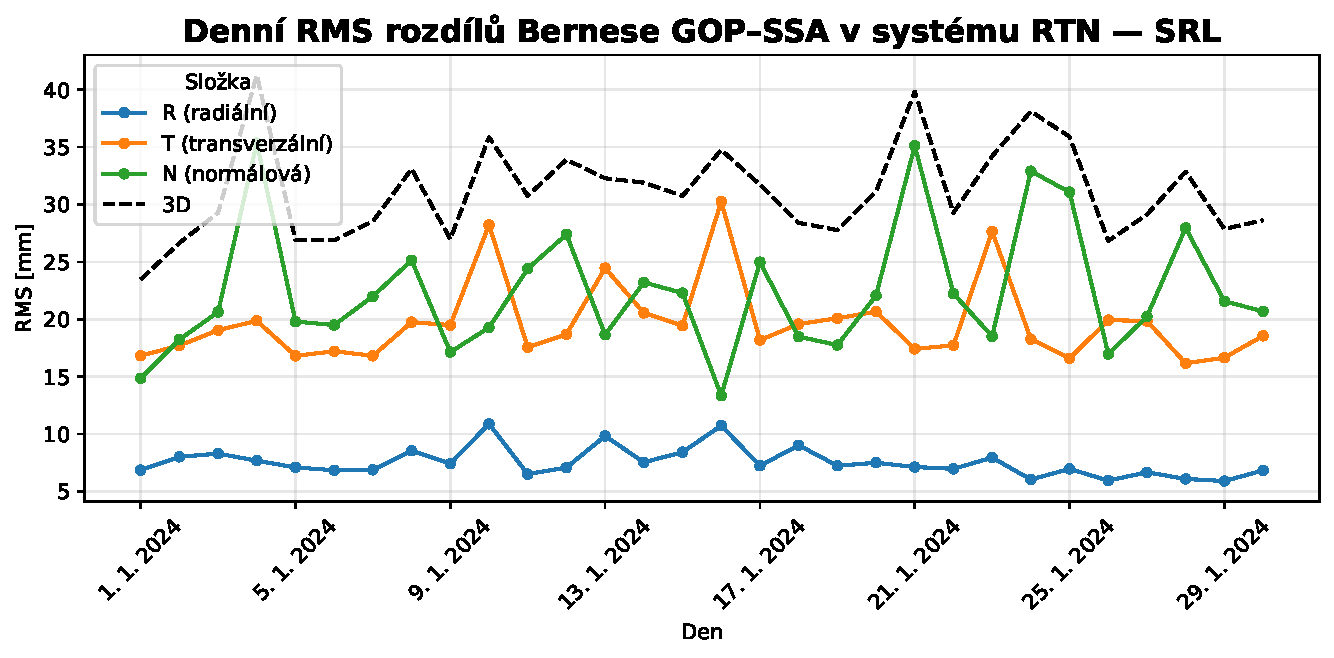
\includegraphics[width=1\textwidth]{images/results/satellites/bernese/sa/sa_ZAZG_doy001-doy030_daily_rtn_3d_rms.pdf}
    \caption{Denní RMS rozdílů \zk{GOP}\,--\,\zk{SSA} získané dynamickou parametrizací}
    \label{fig:srl_bsw_rms_daily}
\end{figure}

Hodnoty jsou prakticky totožné s~výsledky Hermitovy interpolace.

\subsubsection{Srovnání obou přístupů}

Pro přímé srovnání obou metod jsou na~obrázku~\ref{fig:srl_comp_overlay} vykresleny \zk{RTN} rozdíly získané interpolační metodou (modře) a~dynamickou parametrizací (oranžově).

\begin{figure}[H]
    \centering
    
\includegraphics[width=1\textwidth]{images/results/satellites/comparison/srl/hermite_vs_bernese_doy001_rtn_overlay.pdf}
    \caption{Porovnání RTN rozdílů \zk{GOP}\,--\,\zk{SSA} získaných interpolací a parametrizací}
    \label{fig:srl_comp_overlay}
\end{figure}

Z~obrázku je patrné, že obě metody poskytují v~celém průběhu prakticky totožné výsledky ve všech třech složkách \zk{RTN}. Vzájemné odchylky se pohybují na~úrovni jednotek milimetrů, přičemž průběh získaný dynamickou parametrizací je ve srovnání s~interpolační metodou mírně vyhlazenější.

Shoda obou přístupů naznačuje, že pro porovnání přesných drah se vzorkováním 60\,s je Hermitova interpolace plnohodnotnou alternativou k~dynamické parametrizaci a~umožňuje získat srovnatelné výsledky bez nutnosti využití fyzikálního modelu a~softwaru \zkratka{BSW}.

\subsubsection{Interpretace}

Porovnání přesných drah \zk{GOP} a~\zk{SSA} pro družici \zkratka{SARAL} ukazuje, že obě řešení jsou vzájemně konzistentní bez výrazného systematického posunu. Radiální složka~R je nejstabilnější s~průměrnou hodnotou RMS přibližně 8\,mm. Transverzální složka~T dosahuje průměrně přibližně 20\,mm a~normálová složka~N vykazuje největší variabilitu v~rozsahu 14--35\,mm (průměrně $\sim$25\,mm). V~periodogramu jsou přítomny výrazné vrcholy v~oblasti oběžné doby družice \zkratka{SARAL} ($\sim$100\,min), a~to zejména ve složkách N a~T, což naznačuje, že část rozdílů mezi oběma řešeními souvisí s~oběžnou dobou družice. Shoda obou metod porovnání potvrzuje, že zjištěné rozdíly jsou vlastností samotných drahových řešení, nikoli artefaktem zvolené metody analýzy.

\subsection{Souhrnné výsledky}
\label{sec:souhrn-drahy}

Souhrnné hodnoty \zk{RMS} rozdílů drah \zk{GOP}\,--\,\zk{SSA} získané Hermitovou interpolací jsou uvedeny v~tabulce~\ref{tab:gop_vs_ssa_satellites_doy001-doy030_hermite_rms}.

\begin{table}[H]
\centering
\small
\caption{Průměrné RMS rozdílů GOP--SSA získané Hermitovou interpolací}
\label{tab:gop_vs_ssa_satellites_doy001-doy030_hermite_rms}
\begin{tabular}{lrrr}
\toprule
Družice & R [mm] & T [mm] & N [mm] \\
\midrule
SRL & 7.72 & 20.06 & 23.07 \\
CS2 & 9.03 & 26.10 & 24.88 \\
H2C & 9.81 & 28.54 & 37.39 \\
H2D & 8.40 & 33.09 & 28.19 \\
JA3 & 10.24 & 28.21 & 44.14 \\
S3A & 8.48 & 23.41 & 30.56 \\
S3B & 8.30 & 23.34 & 25.71 \\
S6A & 8.14 & 28.78 & 38.60 \\
\bottomrule
\end{tabular}
\end{table}

Dále jsou stručně shrnuty hlavní charakteristiky rozdílů drah pro jednotlivé analyzované družice.

\subsubsection{SARAL}

Rozdíly drah GOP a SSA jsou ve složce R stabilní v~celém analyzovaném období a~pohybují se přibližně v~rozmezí 6--11\,mm. Transverzální složka T dosahuje hodnot přibližně 17--30\,mm a~normálová složka N vykazuje největší variabilitu v~rozsahu přibližně 14--35\,mm. V~periodogramu normálové složky je přítomna dominantní periodicita v~oblasti oběžné doby družice. Obě použité metody -- Hermitova interpolace i~dynamická parametrizace v~softwaru \zkratka{BSW} -- poskytují srovnatelné výsledky s~rozdíly na~úrovni milimetrů.

\subsubsection{CryoSat-2}

CryoSat-2 vykazuje celkově stabilní rozdíly drah \zk{GOP}\,--\,\zk{SSA} v~celém analyzovaném období. Radiální složka R dosahuje hodnot RMS průměrně 8{,}9~mm s~rozsahem přibližně 7--12~mm. Transverzální složka T se pohybuje průměrně kolem 26~mm s~rozsahem přibližně 20--32~mm. Normálová složka N dosahuje průměrně přibližně 24~mm a~vykazuje největší variabilitu v~rozmezí přibližně 18--40~mm. Ke konci ledna 2024 byl ve složce N zaznamenán výraznější nárůst RMS na~hodnotu přibližně 40~mm. V~periodogramu normálové složky je přítomna periodicita odpovídající oběžné době družice ($\sim$99~min). Vzájemné odchylky Hermitovy interpolace a~dynamické parametrizace v~BSW se pohybují na~úrovni jednotek milimetrů.

\subsubsection{HY-2C}

HY-2C vykazuje v~rámci satelitů HY-2 zvýšenou variabilitu normálové složky N. Radiální složka R dosahuje průměrných hodnot RMS přibližně 10~mm s~rozsahem přibližně 6--18~mm. Transverzální složka T se pohybuje kolem 28~mm s~rozsahem přibližně 19--50~mm. Normálová složka N vykazuje největší variabilitu s~průměrnými hodnotami RMS kolem 36~mm a~rozsahem přibližně 15--56~mm. V~periodogramu normálové složky je přítomna dominantní periodicita odpovídající oběžné době družice ($\sim$104~min). Vzájemné odchylky Hermitovy interpolace a~dynamické parametrizace v~BSW se pohybují na~úrovni jednotek milimetrů.

\subsubsection{HY-2D}

HY-2D vykazuje v~průběhu analyzovaného období celkově stabilní rozdíly 
drah. Radiální složka R dosahuje hodnoty RMS průměrně 8{,}1~mm s~rozsahem 
5--17~mm. Transverzální složka T se pohybuje průměrně kolem 28~mm 
s~rozsahem 16--40~mm. V~denních hodnotách RMS byl dne 26.~1.~2024 
zaznamenán výjimečný nárůst na přibližně 100~mm, jehož původ nebyl 
jedno\-značně objasněn. Normálová složka N dosahuje průměrně přibližně 
27~mm s~rozsahem 17--53~mm. V~periodogramu je přítomna periodicita 
odpovídající oběžné době ($\sim$104~min). Vzájemné odchylky Hermitovy 
interpolace a~dynamické parametrizace v~BSW se pohybují na~úrovni 
jednotek milimetrů.

\subsubsection{Jason-3}

Jason-3 vykazuje ze všech analyzovaných satelitů nejvyšší variabilitu normálové složky N. Radiální složka R dosahuje průměrné hodnoty RMS přibližně 10~mm s~rozsahem 7--15~mm. Transverzální složka T se pohybuje průměrně kolem 28~mm s~rozsahem 19--38~mm. Normálová složka N dosahuje průměrné hodnoty RMS 41~mm s~rozsahem 12--84~mm. V~denních hodnotách RMS byl dne 3.~1.~2024 zaznamenán výrazný nárůst na přibližně 84~mm. V~periodogramu je přítomna periodicita odpovídající oběžné době ($\sim$112~min). Celkový charakter rozdílů je analogický k~družici Sentinel-6A, se kterou sdílí orbitální výšku ($\sim$1\,336~km). Vzájemné odchylky Hermitovy interpolace a~dynamické parametrizace v~BSW se pohybují na~úrovni jednotek milimetrů.

\subsubsection{Sentinel-3A}

Sentinel-3A vykazuje stabilní rozdíly drah \zk{GOP}\,--\,\zk{SSA} po celé analyzované 
období. Radiální složka R dosahuje průměrné hodnoty RMS přibližně 8~mm 
s~rozsahem 5--12~mm. Transverzální složka T se pohybuje průměrně kolem 
23~mm s~rozsahem 17--36~mm. Normálová složka N dosahuje průměrné hodnoty 
RMS přibližně 29~mm s~rozsahem 15--52~mm. V~denních hodnotách RMS byl 
kolem 16.~1.~2024 zaznamenán výraznější nárůst na přibližně 52~mm. 
V~periodogramu je přítomna periodicita odpovídající oběžné době 
($\sim$101~min). Výsledky jsou velmi podobné sesterské družici Sentinel-3B, 
což odpovídá totožné orbitální výšce obou satelitů. Vzájemné odchylky 
Hermitovy interpolace a~dynamické parametrizace v~BSW se pohybují 
na~úrovni jednotek milimetrů.

\subsubsection{Sentinel-3B}

Sentinel-3B vykazuje stabilní rozdíly drah \zk{GOP}\,--\,\zk{SSA} velmi podobné 
sesterské družici Sentinel-3A, což odpovídá totožné orbitální výšce 
obou satelitů. Radiální složka R dosahuje průměrné hodnoty RMS přibližně 
8~mm s~rozsahem 6--14~mm. Transverzální složka T se pohybuje průměrně 
kolem 23~mm s~rozsahem 18--37~mm. Normálová složka N dosahuje průměrné 
hodnoty RMS přibližně 25~mm s~rozsahem 14--47~mm. V~denních hodnotách 
RMS byl kolem 25.~1.~2024 zaznamenán výraznější nárůst na přibližně 
47~mm. V~periodogramu je přítomna periodicita odpovídající oběžné době 
($\sim$101~min). Vzájemné odchylky Hermitovy interpolace a~dynamické 
parametrizace v~BSW se pohybují na~úrovni jednotek milimetrů.

\subsubsection{Sentinel-6A}

Sentinel-6A vykazuje vysokou variabilitu normálové složky N analogicky k~družici Jason-3, se kterou sdílí podobnou orbitální výšku ($\sim$1\,336~km). Radiální složka R dosahuje průměrných hodnot RMS přibližně 8~mm s~rozsahem přibližně 5--12~mm. Transverzální složka T se pohybuje kolem 29~mm s~rozsahem přibližně 20--38~mm. Normálová složka N dosahuje průměrných hodnot RMS přibližně 37~mm a~vykazuje největší variabilitu v~rozmezí přibližně 18--79~mm. Dne 11.~1.~2024 byl ve složce N zaznamenán výrazný nárůst RMS na~hodnotu přibližně 79~mm. V~periodogramu jsou přítomny výrazné vrcholy ve složkách N a~T s~dominantní periodicitou v~oblasti oběžné doby družice ($\sim$112~min). Vzájemné odchylky Hermitovy interpolace a~dynamické parametrizace v~BSW se pohybují na~úrovni jednotek milimetrů.
\chapter{Závěr}
\label{8-zaver}

V~rámci této práce byly analyzovány vybrané výsledky zpracování metody \zkratka{DORIS} analytického centra na Geodetické observatoři Pecný VÚGTK. Hodnoceny byly dva typy produktů, a to časové řady souřadnic stanic vysílačů a přesné dráhy družic vybavených přijímači. U~časových řad souřadnic stanic byly za období 2015--2025 posuzovány všechny stanice, u~nichž bylo indikováno podezřelé chování, přičemž pozornost byla věnována zejména dlouhodobým trendům, diskontinuitám a periodickým složkám. Pro analýzu přesných drah družic byly zvoleny družice cs2, h2c, h2d, ja3, s3a, s3b, s6a a srl. Analyzováno bylo prvních třicet dní roku 2024. Cílem bylo porovnat řešení poskytované Geodetickou observatoří Pecný s~řešením \zk{SSA}. Porovnání bylo provedeno dvěma odlišnými přístupy, a to pomocí dynamické parametrizace dráhy v~\zkratka{BSW} a pomocí Hermitovy interpolace souřadnic v~daných epochách. Součástí práce bylo rovněž vytvoření knihovny v~jazyce Python, která umožňuje jednotné zpracování dat systému \zk{DORIS}, jejich analýzu a generování výstupů.

Analýza časových řad souřadnic stanic umožnila posoudit stabilitu vybraných stanic systému \zkratka{DORIS} a identifikovat jejich dlouhodobé trendy, diskontinuity a periodické složky. U~většiny sledovaných stanic bylo indikované podezřelé chování potvrzeno, pravděpodobnou příčinu se však podařilo určit pouze v~některých případech. Nebyly zjištěny zásadní nekonzistence, které by ukazovaly na obecný problém řešení \zk{GOP}. Detekované odchylky mají převážně lokální charakter a jejich interpretace závisí na konkrétní stanici, období a porovnání s~dalšími dostupnými řešeními.

V~části věnované drahám družic bylo provedeno porovnání řešení \zk{GOP} a \zk{SSA} v~lokálním systému \zkratka{RTN}. Výsledky ukázaly, že rozdíly mezi řešeními se většinou pohybují na úrovni centimetrů, přičemž v~radiálním směru, který je u~altimetrických družic často nejdůležitější, dosahují typicky vyšších milimetrů až přibližně 1~cm. Radiální složka současně vykazovala u~všech družic nejnižší a nejstabilnější hodnoty \zk{RMS}, zatímco normálová a transverzální složka dosahovaly vyšších hodnot s~výraznější variabilitou. Ve spektrálních analýzách rozdílů se u~většiny družic projevila periodická složka odpovídající přibližně oběžné době. Oba použité přístupy k~porovnání drah -- Hermitova interpolace a dynamická parametrizace v~\zk{BSW} -- poskytly srovnatelné výsledky se~vzájemnými odchylkami na úrovni jednotek milimetrů, čímž se potvrdila použitelnost interpolační metody.

Výsledky práce přispívají k~hodnocení kvality řešení poskytovaného analytickým centrem na Geodetické observatoři Pecný. Jsou shrnuty výsledky analýzy stability vybraných časových řad souřadnic stanic systému \zkratka{DORIS} a~současně porovnány přesné dráhy družic mezi řešeními \zk{GOP} a~\zk{SSA}. Získané poznatky mají význam pro posouzení spolehlivosti výstupů \zk{GOP}, které jsou využívány mimo jiné při realizaci globálního referenčního rámce (\zk{ITRF}). Vytvořená knihovna umožňuje systema\-tickou analýzu těchto produktů díky jednotnému zpracování dat, porovnání výsledků jednotlivých řešení a~automatizovanému generování výstupů.

Práce je zatížena několika omezeními, která vyplývají jak z~charakteru vstupních dat, tak z~použitých metod. V~případě analýzy časových řad neposkytují některé stanice data za celé analyzované období. U~většiny případů detekovaného nestandardního chování se nepodařilo s~jistotou určit jeho příčinu. Analýza přesných drah družic byla provedena na omezeném časovém úseku, což neumožňuje plně vyhodnotit dlouhodobé chování. Porovnání drah bylo provedeno mezi dvěma nezávislými řešeními. Nalezené rozdíly proto nelze jednoznačně přiřadit ani jednomu z~nich.

Práci je možné dále rozšířit o~analýzu většího počtu stanic a~družic, delších časových období a~dalších řešení analytických center. Vytvořenou knihovnu lze zároveň doplnit o~další metody analýzy. Do budoucna by bylo možné nad knihovnou vytvořit grafické uživatelské rozhraní pro jednodušší analýzu dat.

% Vysázení seznamu zkratek
\begin{seznamzkratek}{}

\novazkratka{DORIS}{DORIS}{Doppler Orbitography and Radiopositioning Integrated by Satellite}

\end{seznamzkratek}

% Literatura
% \nocite{*}
\def\refname{Literatura}
\bibliographystyle{mystyle}
\bibliography{literatura}

% Vysázení seznamu příloh
\seznampriloh

% Vložení souboru s přílohami
% %%%%%%%%%%%%%%%%%%%%%%%%%%%%%%%%%%%%%%%%%%%%%%%%%%%%%%%%%%%%%%%%%%%%%%%%%%%%%%%%%%%
% %%                                    PŘÍLOHY                                    %%
% %%%%%%%%%%%%%%%%%%%%%%%%%%%%%%%%%%%%%%%%%%%%%%%%%%%%%%%%%%%%%%%%%%%%%%%%%%%%%%%%%%%

\appendix
% Příloha A: GitHub repozitář
\chapter*{A GitHub repozitář}
\addcontentsline{loa}{section}{A GitHub repozitář}
\href{https://github.com/kovarmi9/MasterThesis-DorisAnalysis}{\texttt{https://github.com/kovarmi9/MasterThesis-DorisAnalysis}}.
% \begin{center}
% \qrcode[height=4cm]{https://github.com/kovarmi9/BachelorThesis-Astrochronograph}
% \end{center}
% \textbf{Struktura repozitáře:}
% \dirtree{%
% .1 \href{https://github.com/kovarmi9/BachelorThesis-Astrochronograph}{BachelorThesis-Astrochronograph}.
% .2 \href{https://github.com/kovarmi9/BachelorThesis-Astrochronograph/blob/main/README.md}{README.md}.\dottedline  stručná dokumentace.
% .2 \href{https://github.com/kovarmi9/BachelorThesis-Astrochronograph/blob/main/src}{src}.
% .3 \href{https://github.com/kovarmi9/BachelorThesis-Astrochronograph/tree/main/src/Arduino}{Arduino}.\dottedline kódy pro Arduino.
% .4 \href{https://github.com/kovarmi9/BachelorThesis-Astrochronograph/tree/main/src/Arduino/Components}{Components}.\dottedline kódy pro jednotlivé komponenty.
% .5 \href{https://github.com/kovarmi9/BachelorThesis-Astrochronograph/tree/main/src/Arduino/Components/BLE}{BLE}.
% .5 \href{https://github.com/kovarmi9/BachelorThesis-Astrochronograph/tree/main/src/Arduino/Components/Bluetooth}{Bluetooth}.
% .5 \href{https://github.com/kovarmi9/BachelorThesis-Astrochronograph/tree/main/src/Arduino/Components/DCF77_time}{DCF77\_time}.
% .5 \href{https://github.com/kovarmi9/BachelorThesis-Astrochronograph/tree/main/src/Arduino/Components/Display}{Display}.
% .5 \href{https://github.com/kovarmi9/BachelorThesis-Astrochronograph/tree/main/src/Arduino/Components/GNSS_time}{GNSS\_time}.
% .5 \href{https://github.com/kovarmi9/BachelorThesis-Astrochronograph/tree/main/src/Arduino/Components/NTP}{NTP}.
% .5 \href{https://github.com/kovarmi9/BachelorThesis-Astrochronograph/tree/main/src/Arduino/Components/RGB_LED}{RGB\_LED}.
% .5 \href{https://github.com/kovarmi9/BachelorThesis-Astrochronograph/tree/main/src/Arduino/Components/Rotarry_encoder}{Rotarry\_encoder}.
% .5 \href{https://github.com/kovarmi9/BachelorThesis-Astrochronograph/tree/main/src/Arduino/Components/RTC}{RTC}.
% .5 \href{https://github.com/kovarmi9/BachelorThesis-Astrochronograph/tree/main/src/Arduino/Components/SD}{SD}.
% .5 \href{https://github.com/kovarmi9/BachelorThesis-Astrochronograph/tree/main/src/Arduino/Components/Sound}{Sound}.
% .5 \href{https://github.com/kovarmi9/BachelorThesis-Astrochronograph/tree/main/src/Arduino/Components/TS_Reader}{TS\_Reader}.
% .4 \href{https://github.com/kovarmi9/BachelorThesis-Astrochronograph/tree/main/src/Arduino/Complet}{Complet}.\dottedline kompletní kód.
% .5 \href{https://github.com/kovarmi9/BachelorThesis-Astrochronograph/tree/main/src/Arduino/Complet/Astro-Chronograph_R3}{Astrochronograph\_R3}.
% .5 \href{https://github.com/kovarmi9/BachelorThesis-Astrochronograph/tree/main/src/Arduino/Complet/Astro-Chronograph_R4}{Astrochronograph\_R4}.
% .4 \href{https://github.com/kovarmi9/BachelorThesis-Astrochronograph/tree/main/src/Arduino/Test}{Test}.\dottedline kód pro testování.
% .3 \href{https://github.com/kovarmi9/BachelorThesis-Astrochronograph/tree/main/src/LaTeX}{LaTeX}.\dottedline zdrojový kód práce ve formátu \LaTeX.
% .3 \href{https://github.com/kovarmi9/BachelorThesis-Astrochronograph/tree/main/src/R}{R}.\dottedline zpracování testovacích dat.
% .2 \href{https://github.com/kovarmi9/BachelorThesis-Astrochronograph/tree/main/Eagle}{Eagle}.\dottedline schéma zapojení a návrh DPS.
% .2 \href{https://github.com/kovarmi9/BachelorThesis-Astrochronograph/tree/main/Text}{Text}.
% .3 \href{https://github.com/kovarmi9/BachelorThesis-Astrochronograph/blob/main/Text/Thesis.pdf}{Thesis.pdf}.\dottedline text práce ve formátu PDF.
% .3 \href{https://github.com/kovarmi9/BachelorThesis-Astrochronograph/blob/main/Text/Presentation.pdf}{Presentation.pdf}.\dottedline Prezentace ve formátu PDF.
% }

% % Příloha B: Elektronická příloha - SD karta
% \newpage
% \chapter*{B Elektronická příloha - SD karta}
% \addcontentsline{loa}{section}{B Elektronická příloha - SD karta}
% \textbf{Struktura souborů na SD kartě:}
% \dirtree{%
% .1 SD.
% .2 Arduino.\dottedline kódy pro Arduino.
% .3 Components.\dottedline kódy pro jednotlivé komponenty.
% .4 BLE.
% .4 Bluetooth.
% .4 DCF77\_time.
% .4 Display.
% .4 GNSS\_time.
% .4 NTP.
% .4 RGB\_LED.
% .4 Rotarry\_encoder.
% .4 RTC.
% .4 SD.
% .4 Sound.
% .4 TS\_Reader.
% .3 Complet.\dottedline kompletní kód.
% .4 Astrochronograph\_R3.
% .4 Astrochronograph\_R4.
% .3 Test.
% .2 R.\dottedline zpracování testovacích dat.
% .2 Eagle.\dottedline schéma zapojení a návrh DPS.
% }

% Konec dokumentu
\end{document}